% !TEX encoding = UTF-8
% !TEX TS-program = pdflatex
% !TEX root = ../Articolo.tex
% !TEX spellcheck = it-IT

%************************************************
\section{Model Identification}
\label{sec:modelidentification}
%************************************************

Specific operating ranges  in N/alpha domain:
\begin{itemize}
	\item{Identification data: JKU DOE 2, augmented Ferrari cycle ($data_acq_tuesday_augFcycle001$).}
	\item{Validation data: JKU DOE 1 ($data_acq_tuesday_jkucycle001$).}
\end{itemize}



\subsection{Turbocharger Right Way Out Air Pressure (P2 Dx)}
\begin{itemize}
	\item{inputs: actual engine torque (copp kgm), ingnition angle (zwout)}
	\item{output: turbocharger right way out air pressure (p2 dx)}
\end{itemize}	

\begin{landscape}
\begin{center} 
\footnotesize
\begin{longtable}{ll|cccc|ccc|ccc} 
\caption[inputs COPP KGM zwout   outputs P2 DX]{inputs COPP KGM zwout   outputs P2 DX.} 
\label{tab:inputs_COPP_KGM_zwout___outputs_P2_DX} 
\hline 
  mdl & type & np & nz & dPl & oY & ft100 & mxDf100 & mse100 & ft200 & mxDf200 & mse200 \\ 
 \hline 
tf  & iden & 1 & 1 & 0 & 0 & 58.1 & 0.47 & 0.00 & 52.8 & 0.46 & 0.00 \\ 
tf  & sim & 1 & 1 & 0 & 0 & 31.3 & 0.46 & 0.00 & 29.9 & 0.52 & 0.00 \\ 
 \hline 
tf  & iden & 1 & 2 & 0 & 0 & 58.5 & 0.40 & 0.00 & 52.8 & 0.45 & 0.00 \\ 
tf  & sim & 1 & 2 & 0 & 0 & 34.0 & 0.43 & 0.00 & 30.2 & 0.53 & 0.00 \\ 
 \hline 
tf  & iden & 2 & 1 & 0 & 0 & 57.9 & 0.41 & 0.00 & 51.4 & 0.40 & 0.00 \\ 
tf  & sim & 2 & 1 & 0 & 0 & 30.8 & 0.47 & 0.00 & 40.3 & 0.47 & 0.00 \\ 
 \hline 
tf  & iden & 2 & 2 & 0 & 0 & 58.9 & 0.40 & 0.00 & 53.3 & 0.42 & 0.00 \\ 
tf  & sim & 2 & 2 & 0 & 0 & 34.3 & 0.42 & 0.00 & 31.3 & 0.52 & 0.00 \\ 
 \hline 
narx & iden & 0 & 1 & 1 & 1 & 85.6 & 0.27 & 0.00 & 76.7 & 0.35 & 0.00 \\ 
narx & pred & 0 & 1 & 1 & 1 & 82.5 & 0.32 & 0.03 & 71.3 & 0.31 & 0.05 \\ 
narx & sim & 0 & 1 & 1 & 1 & 8.6 & 0.49 & 0.17 & 18.6 & 0.44 & 0.15 \\ 
 \hline 
narx & iden & 0 & 1 & 2 & 1 & 85.6 & 0.27 & 0.00 & 77.5 & 0.35 & 0.00 \\ 
narx & pred & 0 & 1 & 2 & 1 & 82.6 & 0.32 & 0.03 & 49.8 & 0.35 & 0.09 \\ 
narx & sim & 0 & 1 & 2 & 1 & 0.3 & 0.52 & 0.18 & 0.0 & 9.99 & 9.99 \\ 
 \hline 
narx & iden & 0 & 1 & 3 & 1 & 86.4 & 0.25 & 0.00 & 79.9 & 0.34 & 0.00 \\ 
narx & pred & 0 & 1 & 3 & 1 & 70.5 & 0.82 & 0.05 & 40.4 & 1.75 & 0.11 \\ 
narx & sim & 0 & 1 & 3 & 1 & 0.0 & 9.99 & 9.99 & 0.0 & 9.99 & 9.99 \\ 
 \hline 
narx & iden & 0 & 1 & 4 & 1 & 87.0 & 0.26 & 0.00 & 81.5 & 0.32 & 0.00 \\ 
narx & pred & 0 & 1 & 4 & 1 & 16.2 & 3.51 & 0.15 & 0.0 & 5.70 & 0.28 \\ 
narx & sim & 0 & 1 & 4 & 1 & 0.0 & 9.99 & 9.99 & 0.0 & 9.99 & 9.99 \\ 
 \hline 
narx & iden & 0 & 1 & 1 & 2 & 87.6 & 0.29 & 0.00 & 78.1 & 0.38 & 0.00 \\ 
narx & pred & 0 & 1 & 1 & 2 & 84.0 & 0.36 & 0.03 & 73.5 & 0.31 & 0.05 \\ 
narx & sim & 0 & 1 & 1 & 2 & 24.0 & 0.52 & 0.14 & 25.4 & 0.44 & 0.14 \\ 
 \hline 
narx & iden & 0 & 1 & 2 & 2 & 87.7 & 0.29 & 0.00 & 78.8 & 0.35 & 0.00 \\ 
narx & pred & 0 & 1 & 2 & 2 & 83.9 & 0.39 & 0.03 & 57.8 & 0.34 & 0.08 \\ 
narx & sim & 0 & 1 & 2 & 2 & 20.0 & 0.42 & 0.15 & 0.0 & 9.99 & 9.99 \\ 
 \hline 
narx & iden & 0 & 1 & 3 & 2 & 89.0 & 0.28 & 0.00 & 82.0 & 0.37 & 0.00 \\ 
narx & pred & 0 & 1 & 3 & 2 & 76.7 & 0.46 & 0.04 & 40.0 & 1.76 & 0.11 \\ 
narx & sim & 0 & 1 & 3 & 2 & 0.0 & 9.99 & 9.99 & 0.0 & 9.99 & 9.99 \\ 
 \hline 
narx & iden & 0 & 1 & 4 & 2 & 89.9 & 0.29 & 0.00 & 84.6 & 0.28 & 0.00 \\ 
narx & pred & 0 & 1 & 4 & 2 & 34.6 & 2.91 & 0.12 & 0.0 & 7.43 & 0.33 \\ 
narx & sim & 0 & 1 & 4 & 2 & 0.0 & 9.99 & 9.99 & 0.0 & 9.99 & 9.99 \\ 
 \hline 
narx & iden & 0 & 1 & 1 & 3 & 87.6 & 0.29 & 0.00 & 78.1 & 0.38 & 0.00 \\ 
narx & pred & 0 & 1 & 1 & 3 & 84.0 & 0.37 & 0.03 & 73.5 & 0.31 & 0.05 \\ 
narx & sim & 0 & 1 & 1 & 3 & 22.4 & 0.52 & 0.14 & 25.4 & 0.44 & 0.14 \\ 
 \hline 
narx & iden & 0 & 1 & 2 & 3 & 88.0 & 0.29 & 0.00 & 78.8 & 0.35 & 0.00 \\ 
narx & pred & 0 & 1 & 2 & 3 & 84.2 & 0.39 & 0.03 & 57.8 & 0.34 & 0.08 \\ 
narx & sim & 0 & 1 & 2 & 3 & 12.6 & 0.42 & 0.16 & 0.0 & 9.99 & 9.99 \\ 
 \hline 
narx & iden & 0 & 1 & 3 & 3 & 89.3 & 0.30 & 0.00 & 82.5 & 0.36 & 0.00 \\ 
narx & pred & 0 & 1 & 3 & 3 & 77.0 & 0.34 & 0.04 & 40.0 & 1.68 & 0.11 \\ 
narx & sim & 0 & 1 & 3 & 3 & 0.0 & 9.99 & 9.99 & 0.0 & 9.99 & 9.99 \\ 
 \hline 
narx & iden & 0 & 1 & 4 & 3 & 0.0 & 0.00 & 0.00 & 85.4 & 0.27 & 0.00 \\ 
narx & pred & 0 & 1 & 4 & 3 & 0.0 & 0.00 & 0.00 & 0.0 & 5.97 & 0.28 \\ 
narx & sim & 0 & 1 & 4 & 3 & 0.0 & 0.00 & 0.00 & 0.0 & 9.99 & 9.99 \\ 
 \hline 
narx & iden & 0 & 2 & 1 & 1 & 89.4 & 0.20 & 0.00 & 84.5 & 0.23 & 0.00 \\ 
narx & pred & 0 & 2 & 1 & 1 & 85.5 & 0.21 & 0.03 & 79.9 & 0.23 & 0.04 \\ 
narx & sim & 0 & 2 & 1 & 1 & 0.0 & 0.56 & 0.29 & 49.4 & 0.27 & 0.09 \\ 
 \hline 
narx & iden & 0 & 2 & 2 & 1 & 0.0 & 0.00 & 0.00 & 86.0 & 0.19 & 0.00 \\ 
narx & pred & 0 & 2 & 2 & 1 & 0.0 & 0.00 & 0.00 & 64.7 & 0.21 & 0.06 \\ 
narx & sim & 0 & 2 & 2 & 1 & 0.0 & 0.00 & 0.00 & 0.0 & 9.99 & 9.99 \\ 
 \hline 
narx & iden & 0 & 2 & 3 & 1 & 0.0 & 0.00 & 0.00 & 88.3 & 0.16 & 0.00 \\ 
narx & pred & 0 & 2 & 3 & 1 & 0.0 & 0.00 & 0.00 & 18.6 & 0.57 & 0.15 \\ 
narx & sim & 0 & 2 & 3 & 1 & 0.0 & 0.00 & 0.00 & 0.0 & 9.99 & 9.99 \\ 
 \hline 
narx & iden & 0 & 2 & 1 & 2 & 89.5 & 0.20 & 0.00 & 84.5 & 0.22 & 0.00 \\ 
narx & pred & 0 & 2 & 1 & 2 & 85.8 & 0.21 & 0.03 & 79.5 & 0.24 & 0.04 \\ 
narx & sim & 0 & 2 & 1 & 2 & 23.2 & 0.36 & 0.14 & 48.0 & 0.27 & 0.10 \\ 
 \hline 
narx & iden & 0 & 2 & 2 & 2 & 0.0 & 0.00 & 0.00 & 86.3 & 0.18 & 0.00 \\ 
narx & pred & 0 & 2 & 2 & 2 & 0.0 & 0.00 & 0.00 & 59.4 & 0.26 & 0.07 \\ 
narx & sim & 0 & 2 & 2 & 2 & 0.0 & 0.00 & 0.00 & 0.0 & 9.99 & 9.99 \\ 
 \hline 
narx & iden & 0 & 2 & 3 & 2 & 0.0 & 0.00 & 0.00 & 89.5 & 0.17 & 0.00 \\ 
narx & pred & 0 & 2 & 3 & 2 & 0.0 & 0.00 & 0.00 & 0.0 & 1.76 & 0.24 \\ 
narx & sim & 0 & 2 & 3 & 2 & 0.0 & 0.00 & 0.00 & 0.0 & 9.99 & 9.99 \\ 
 \hline 
narx & iden & 0 & 2 & 1 & 3 & 89.6 & 0.20 & 0.00 & 84.5 & 0.22 & 0.00 \\ 
narx & pred & 0 & 2 & 1 & 3 & 85.7 & 0.23 & 0.03 & 79.5 & 0.24 & 0.04 \\ 
narx & sim & 0 & 2 & 1 & 3 & 12.4 & 0.38 & 0.16 & 48.0 & 0.27 & 0.10 \\ 
 \hline 
narx & iden & 0 & 2 & 2 & 3 & 0.0 & 0.00 & 0.00 & 86.4 & 0.18 & 0.00 \\ 
narx & pred & 0 & 2 & 2 & 3 & 0.0 & 0.00 & 0.00 & 59.8 & 0.26 & 0.07 \\ 
narx & sim & 0 & 2 & 2 & 3 & 0.0 & 0.00 & 0.00 & 0.0 & 9.99 & 9.99 \\ 
 \hline 
narx & iden & 0 & 2 & 3 & 3 & 0.0 & 0.00 & 0.00 & 90.0 & 0.16 & 0.00 \\ 
narx & pred & 0 & 2 & 3 & 3 & 0.0 & 0.00 & 0.00 & 0.0 & 2.21 & 0.29 \\ 
narx & sim & 0 & 2 & 3 & 3 & 0.0 & 0.00 & 0.00 & 0.0 & 9.99 & 9.99 \\ 
 \hline 
\end{longtable} 
\normalsize
\end{center}
\end{landscape}

%%inputsCOPP_KGM-zwout-outputsP2_DX-1

\begin{figure}[htbp]
	\centering 
	\subfloat[P2 DX: Narx identification]{ %[trim=left bottom right top, clip]{
		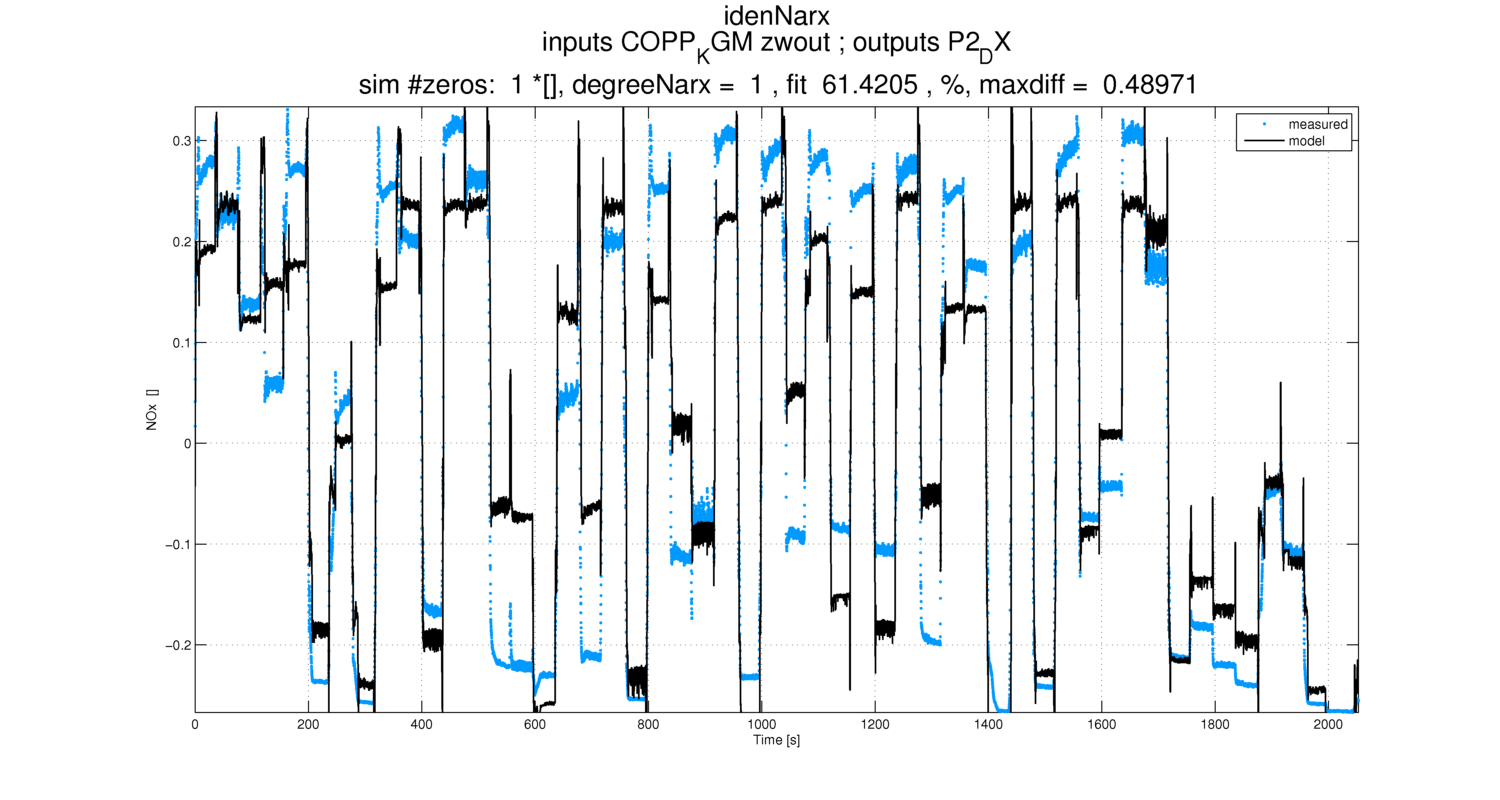
\includegraphics[trim = 30mm 5mm 30mm 0mm, clip, width=.9\columnwidth]{Immagini/inputsCOPP_KGMzwoutoutputsP2_DX-idenNarx-1}
		\label{fig:inputsCOPP_KGMzwoutoutputsP2_DX-idenNarx-1}	}
	\\
	\subfloat[P2 DX: Narx prediction]{
		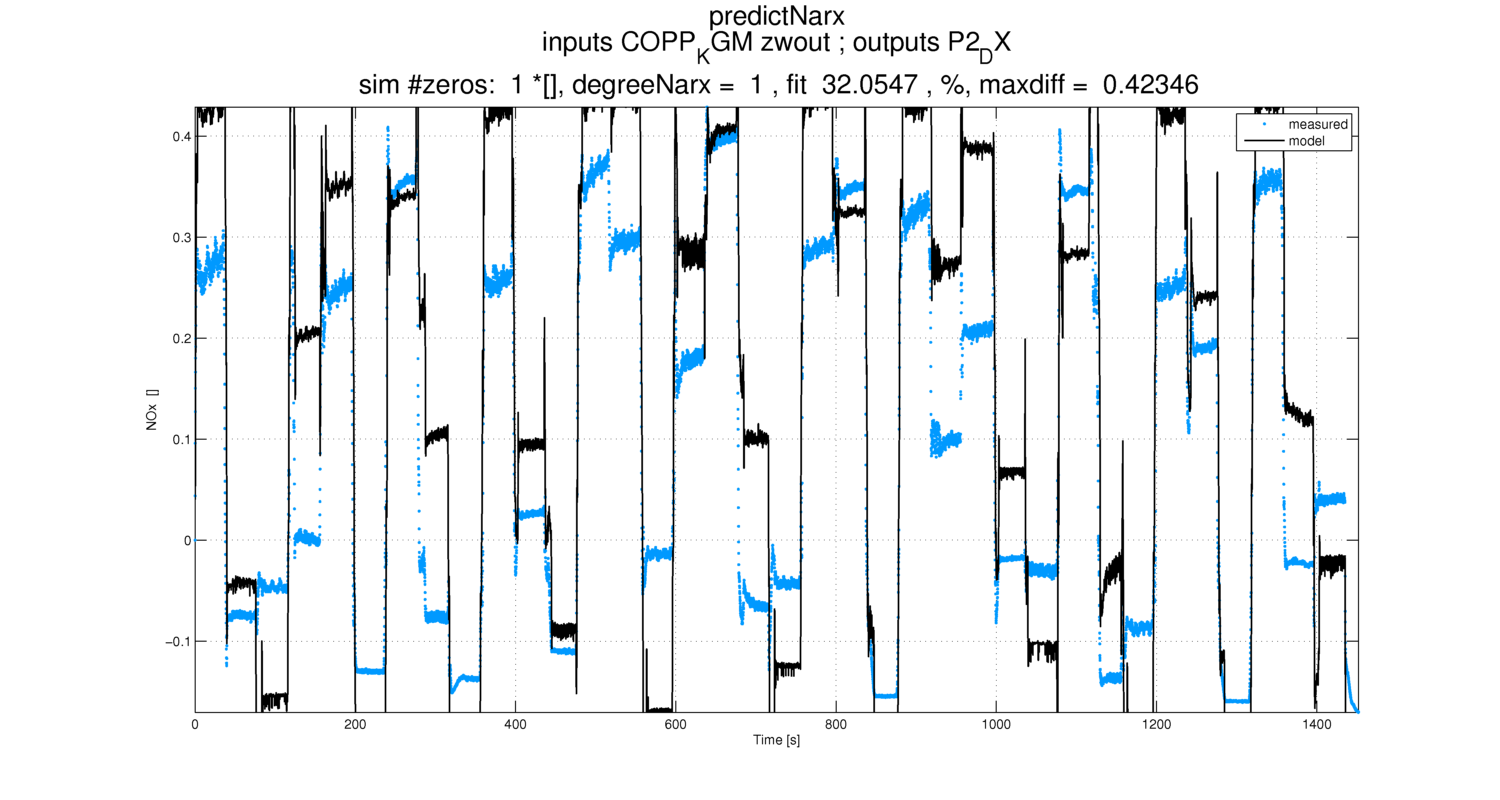
\includegraphics[trim = 30mm 5mm 30mm 0mm, clip, width=.9\columnwidth]{Immagini/inputsCOPP_KGMzwoutoutputsP2_DX-predictNarx-1}
		\label{fig:inputsCOPP_KGMzwoutoutputsP2_DX-predictNarx-1}
	}
	\\
	\subfloat[P2 DX: Narx simulation]{
		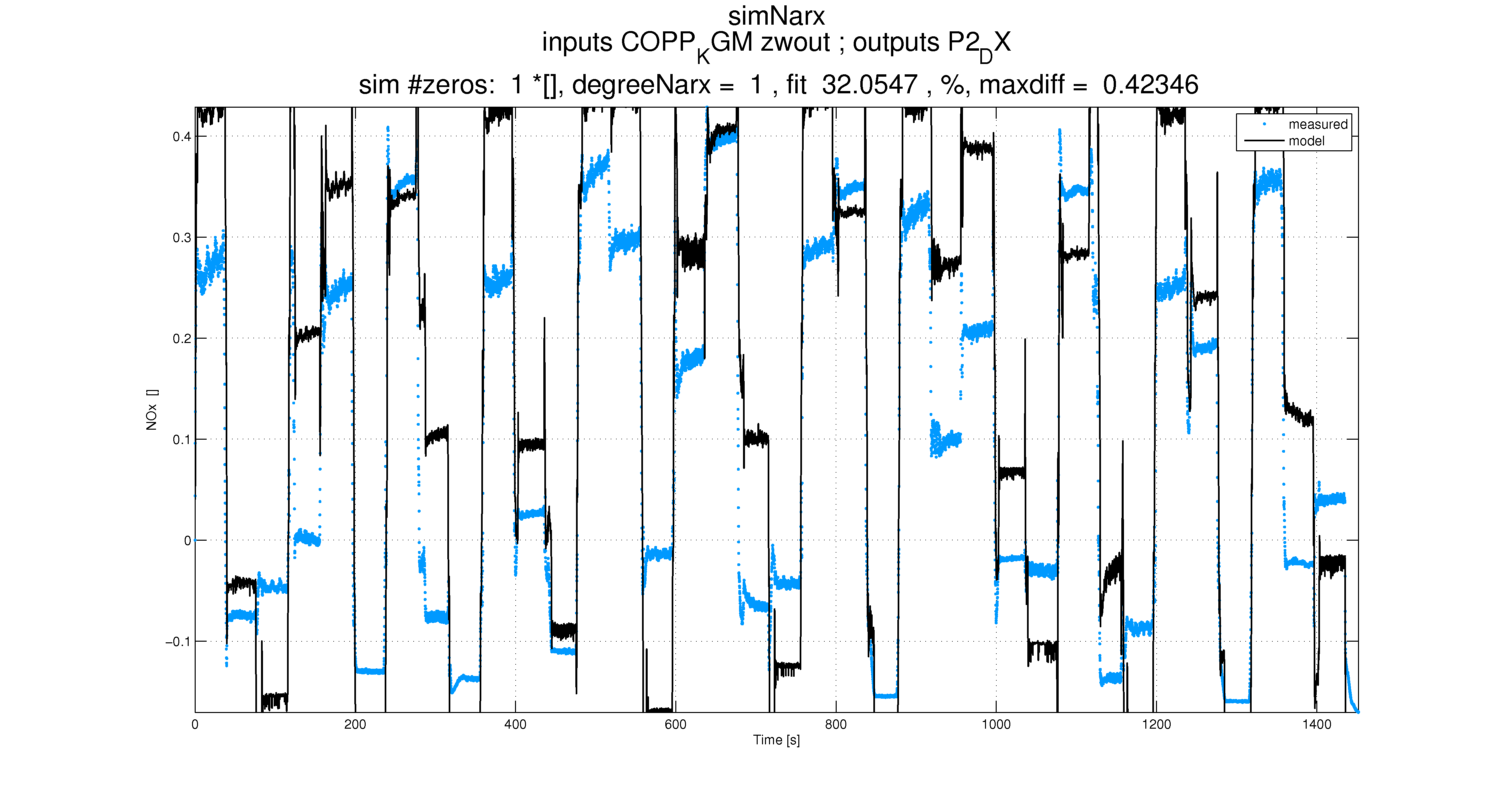
\includegraphics[trim = 30mm 5mm 30mm 0mm, clip, width=.9\columnwidth]{Immagini/inputsCOPP_KGMzwoutoutputsP2_DX-simNarx-1}
		\label{fig:inputsCOPP_KGMzwoutoutputsP2_DX-simNarx-1}
	}
\phantomcaption
\end{figure}


\begin{figure}[htbp] \ContinuedFloat
	\centering 
	\subfloat[P2 DX: Transfer function identification]{
		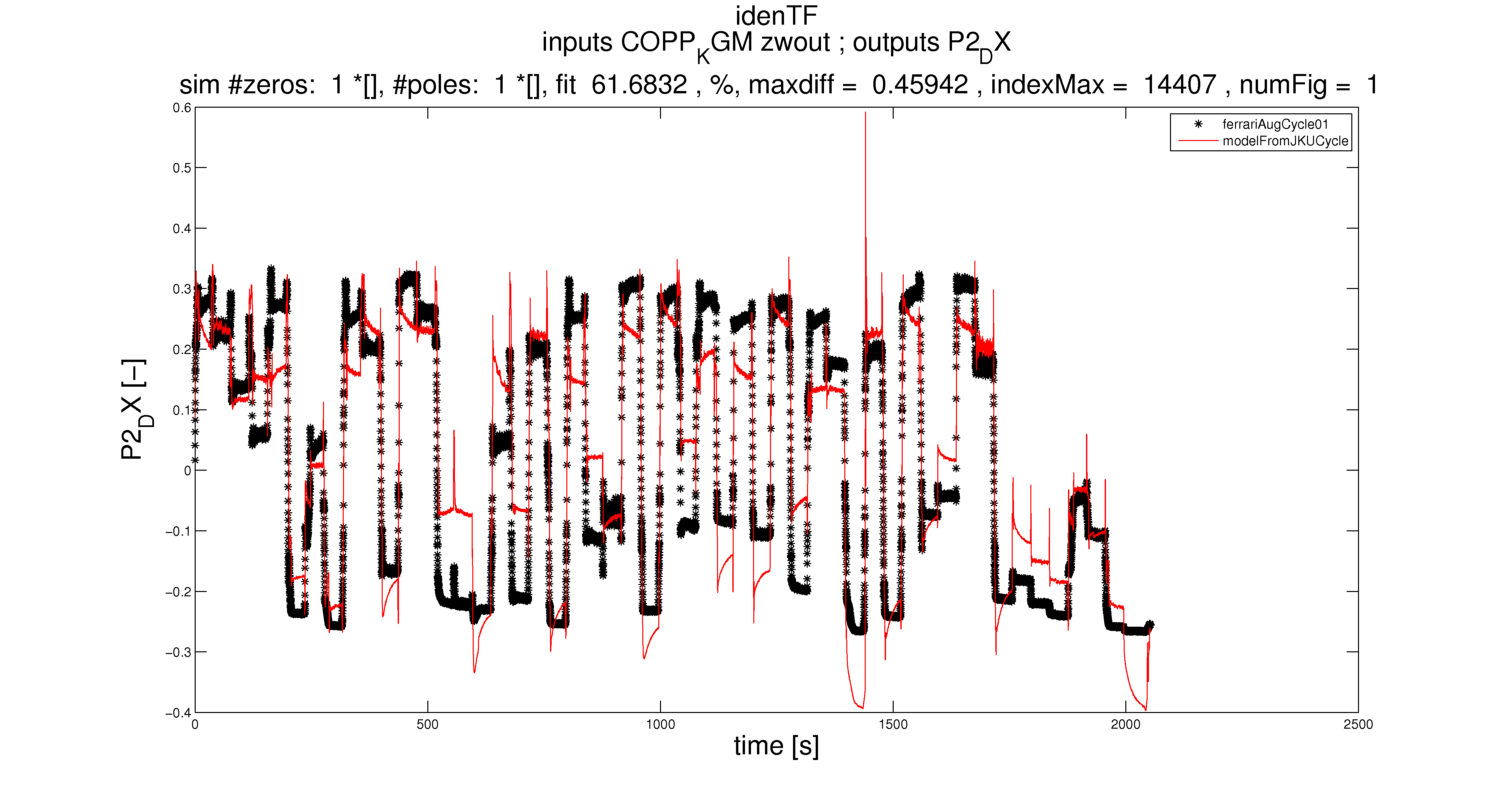
\includegraphics[trim = 30mm 5mm 30mm 0mm, clip, width=.9\columnwidth]{Immagini/inputsCOPP_KGMzwoutoutputsP2_DX-idenTF-1}
		\label{fig:inputsCOPP_KGMzwoutoutputsP2_DX-idenTF-1}  }
	\\
	\subfloat[P2 DX: Transfer function simulation]{
		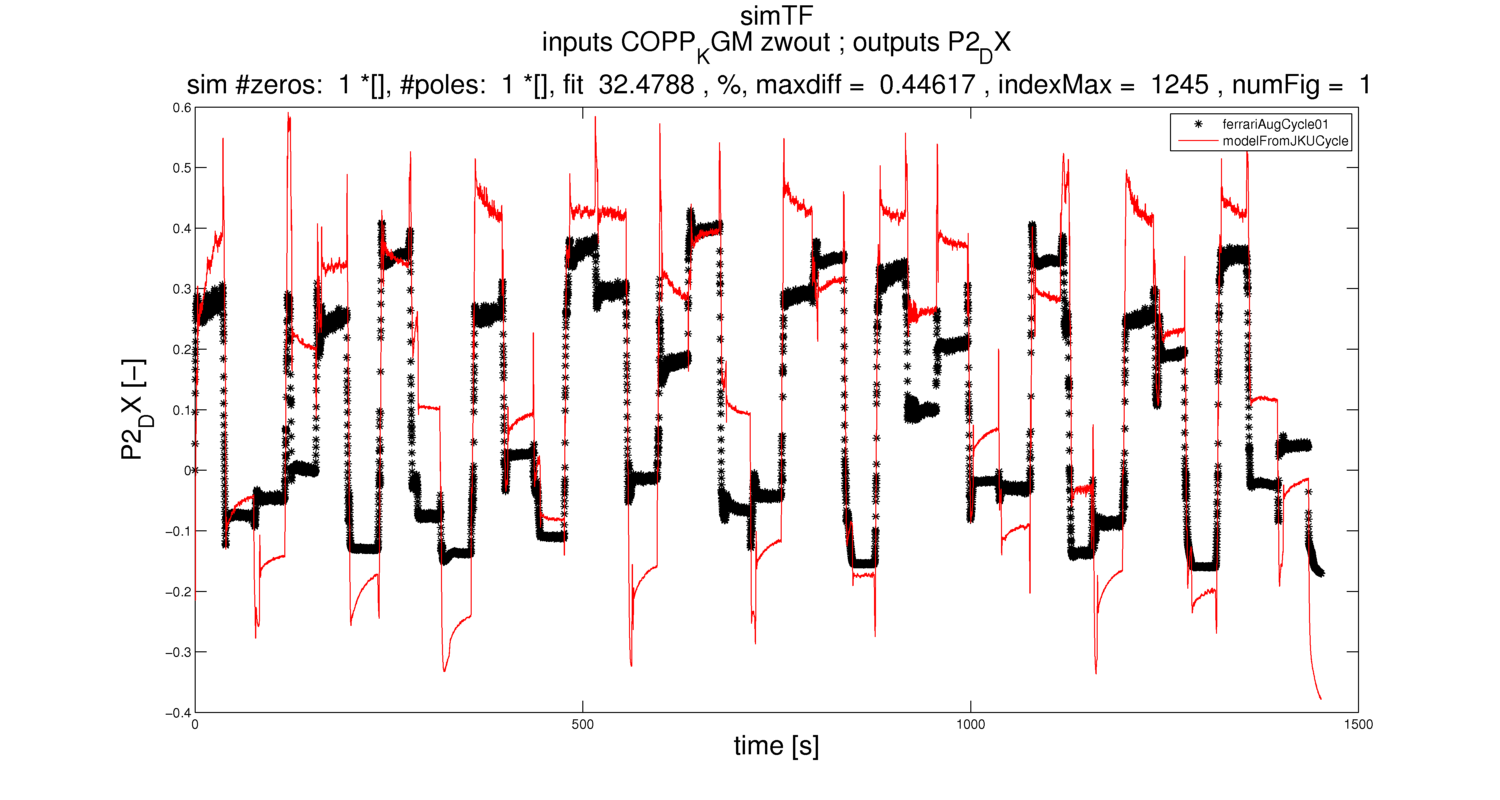
\includegraphics[trim = 30mm 5mm 30mm 0mm, clip, width=.9\columnwidth]{Immagini/inputsCOPP_KGMzwoutoutputsP2_DX-simTF-1}
		\label{fig:inputsCOPP_KGMzwoutoutputsP2_DX-simTF-1}  }
	\\	

	\caption[Inputs: COPP KGM, zwout; Output: P2DX; np: 1; nz: 1; degree: 1]{Inputs: COPP KGM, zwout; Output: P2DX; np: 1; nz: 1; degree: 1}
	\label{fig:inputsCOPP_KGM-zwout-outputsP2_DX-1}
\end{figure}
%%inputsCOPP_KGM-zwout-outputsP2_DX-2

\begin{figure}[htbp]
	\centering 
	\subfloat[P2 DX: Narx identification]{
		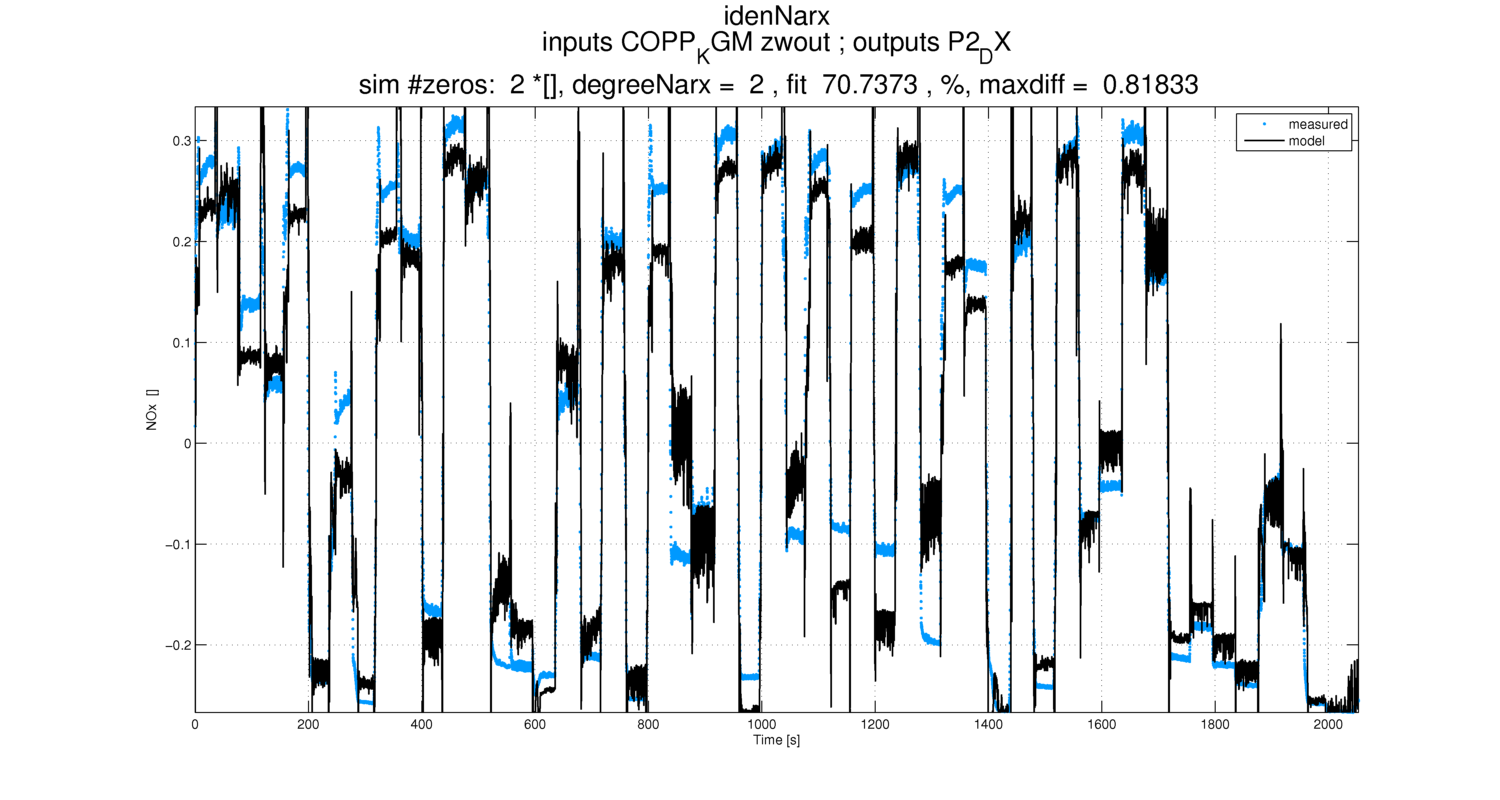
\includegraphics[width=.9\columnwidth]{Immagini/inputsCOPP_KGMzwoutoutputsP2_DX-idenNarx-2}
		\label{fig:inputsCOPP_KGMzwoutoutputsP2_DX-idenNarx-2}	}
	\\
	\subfloat[P2 DX: Narx prediction]{
		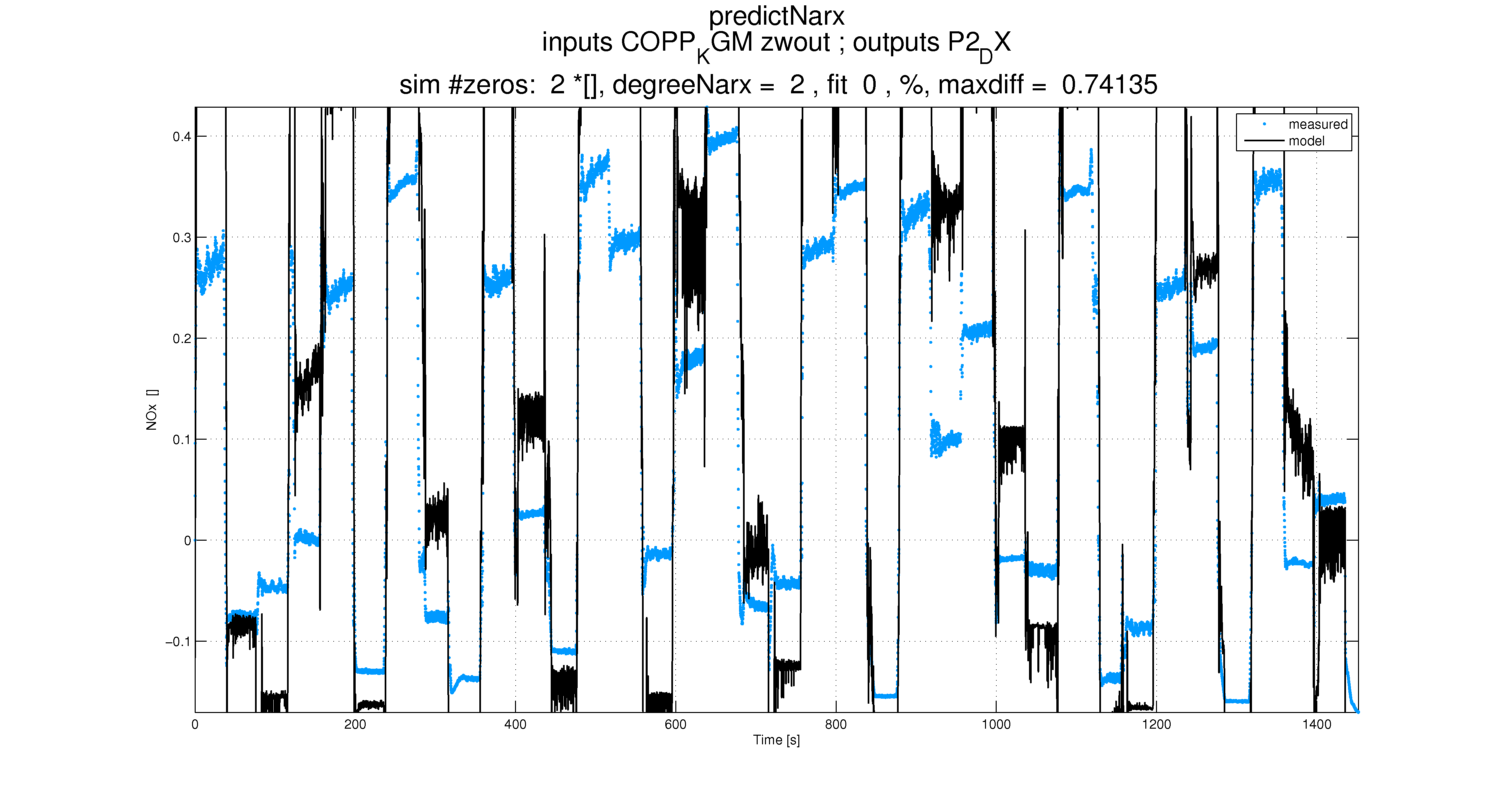
\includegraphics[width=.9\columnwidth]{Immagini/inputsCOPP_KGMzwoutoutputsP2_DX-predictNarx-2}
		\label{fig:inputsCOPP_KGMzwoutoutputsP2_DX-predictNarx-2}
	}
	\\
	\subfloat[P2 DX: Narx simulation]{
		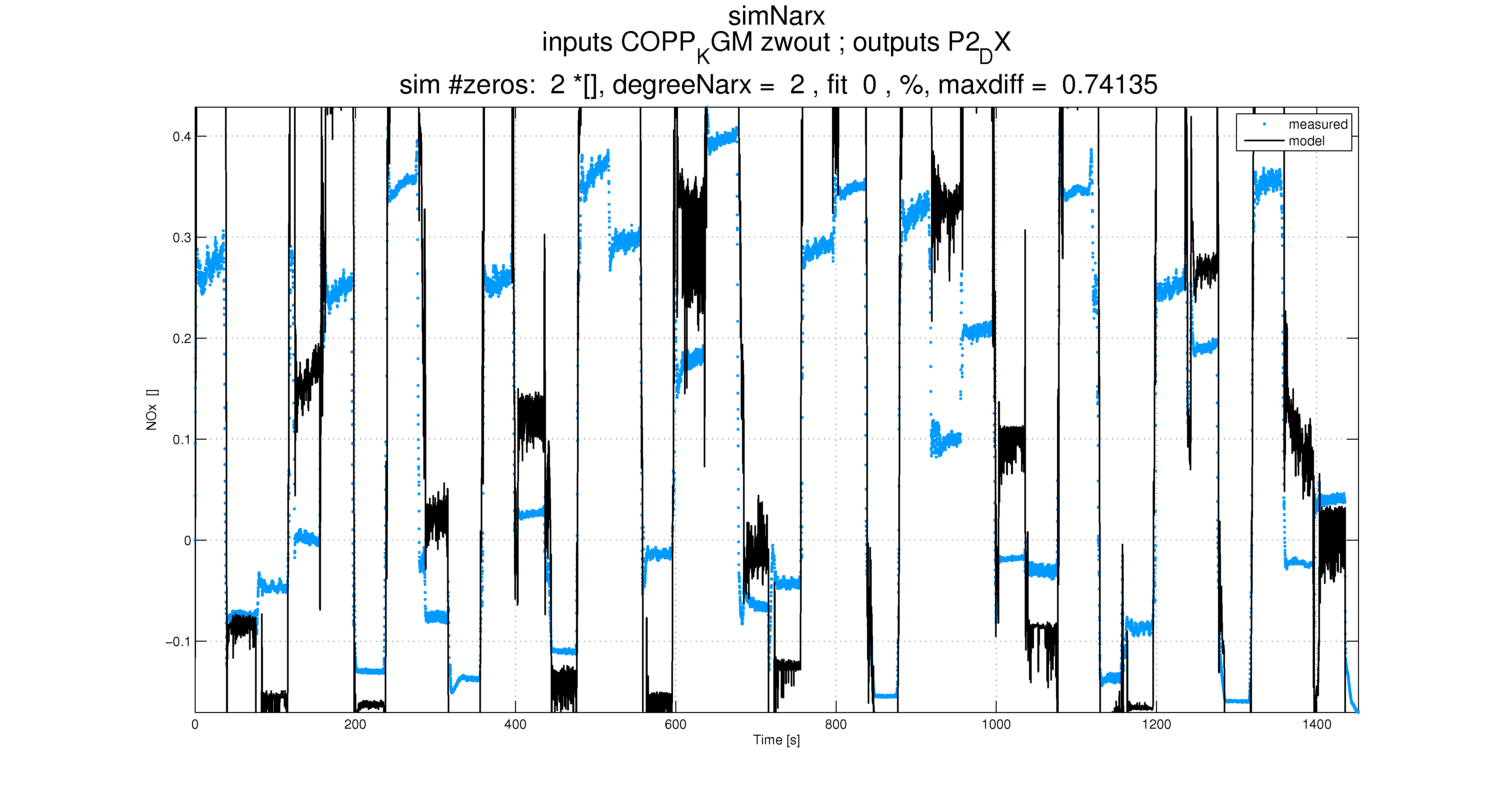
\includegraphics[width=.9\columnwidth]{Immagini/inputsCOPP_KGMzwoutoutputsP2_DX-simNarx-2}
		\label{fig:inputsCOPP_KGMzwoutoutputsP2_DX-simNarx-2}
	}
\phantomcaption
\end{figure}


\begin{figure}[htbp] \ContinuedFloat
	\centering 
	\subfloat[P2 DX: Transfer function identification]{
		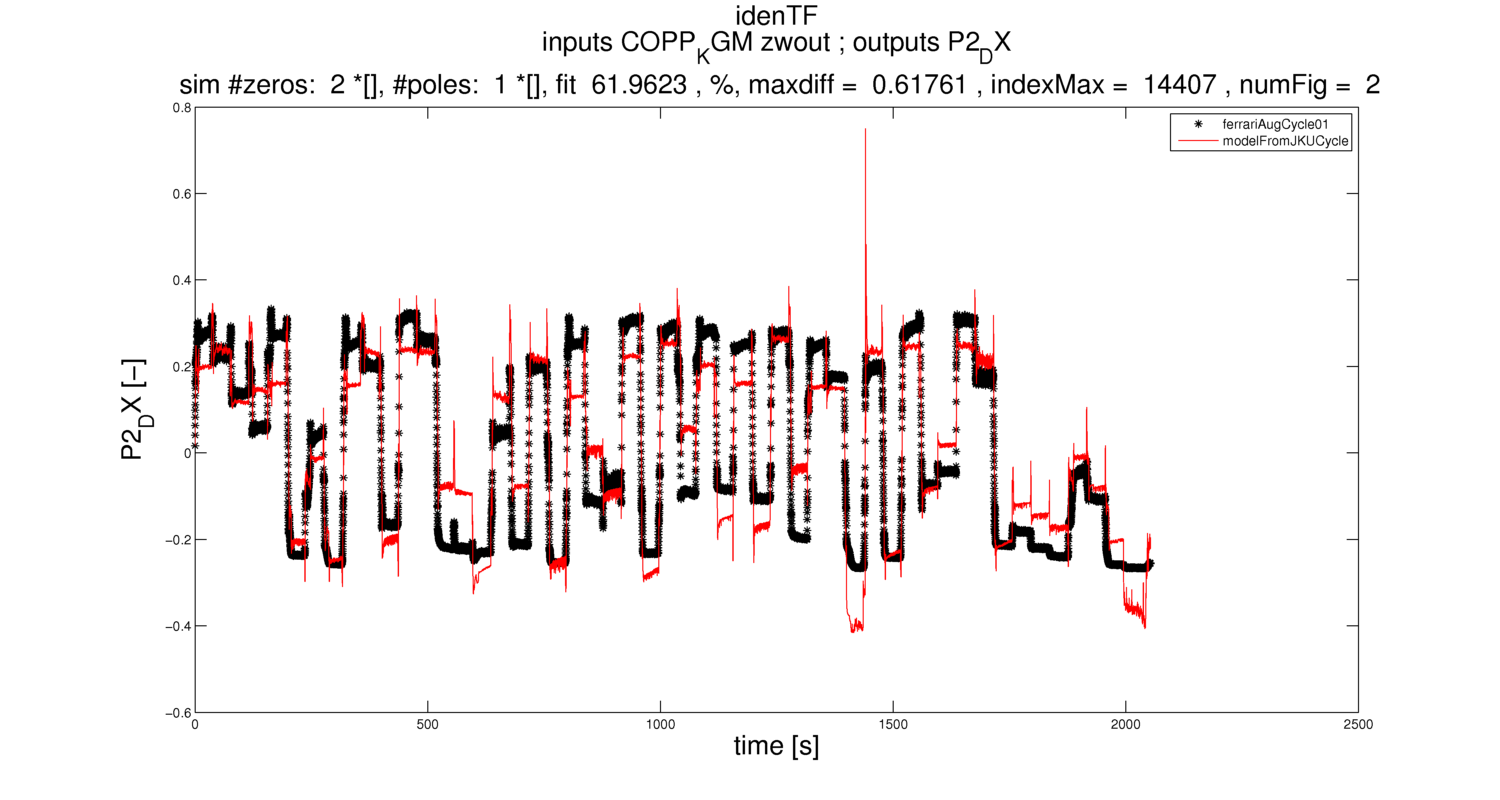
\includegraphics[width=.9\columnwidth]{Immagini/inputsCOPP_KGMzwoutoutputsP2_DX-idenTF-2}
		\label{fig:inputsCOPP_KGMzwoutoutputsP2_DX-idenTF-12}  }
	\\
	\subfloat[P2 DX: Transfer function simulation]{
		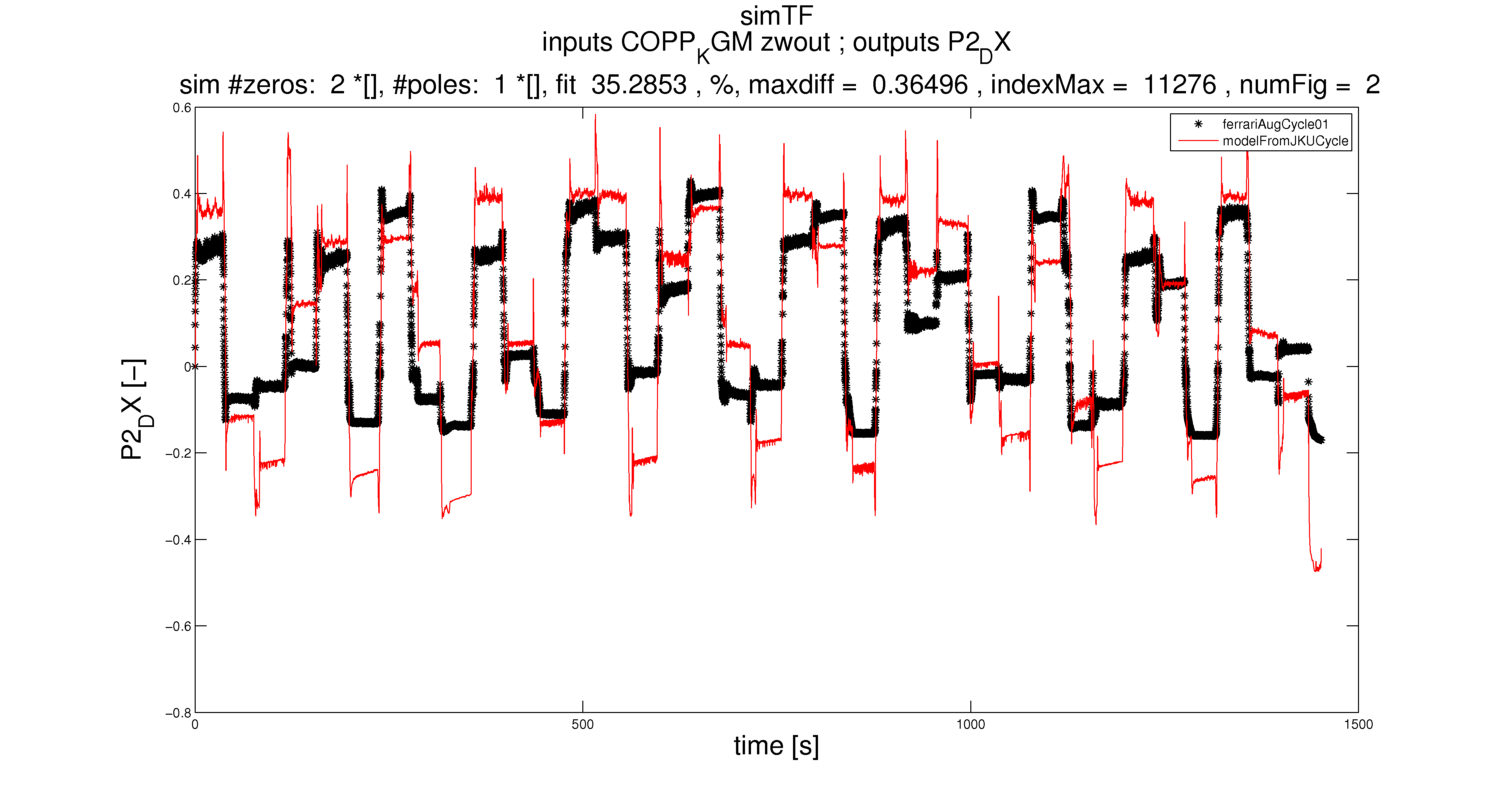
\includegraphics[width=.9\columnwidth]{Immagini/inputsCOPP_KGMzwoutoutputsP2_DX-simTF-2}
		\label{fig:inputsCOPP_KGMzwoutoutputsP2_DX-simTF-2}  }
	\\	

	\caption[Inputs: COPP KGM, zwout; Output: P2DX; np: 1; nz: 2; degree: 1]{Inputs: COPP KGM, zwout; Output: P2DX; np: 1; nz: 2; degree: 1}
	\label{fig:inputsCOPP_KGM-zwout-outputsP2_DX-2}	
\end{figure}
%%inputsCOPP_KGM-zwout-outputsP2_DX-3

\begin{figure}[htbp]
	\centering 
	\subfloat[P2 DX: Narx identification]{
		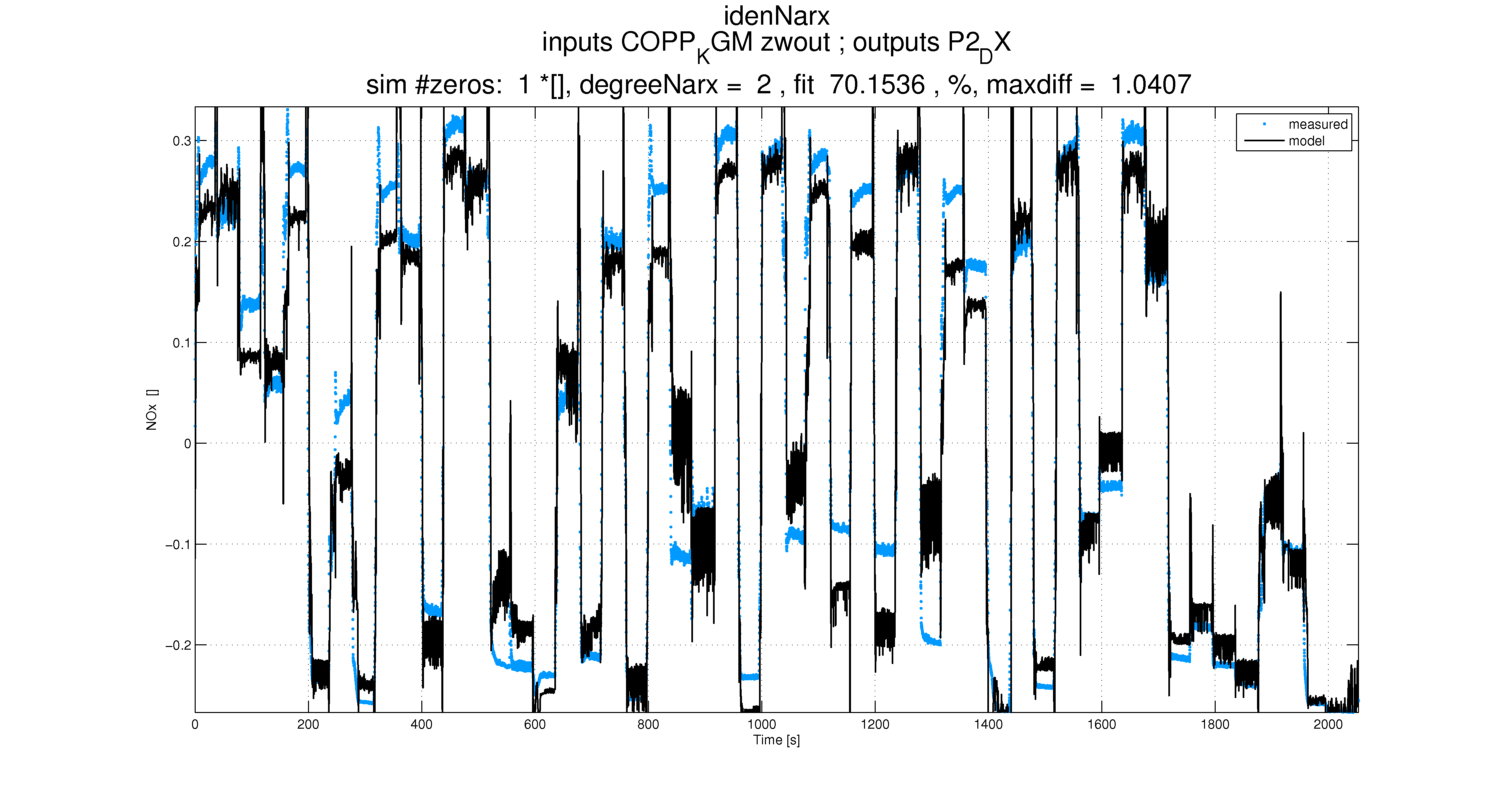
\includegraphics[width=.9\columnwidth]{Immagini/inputsCOPP_KGMzwoutoutputsP2_DX-idenNarx-3}
		\label{fig:inputsCOPP_KGMzwoutoutputsP2_DX-idenNarx-3}	}
	\\
	\subfloat[P2 DX: Narx prediction]{
		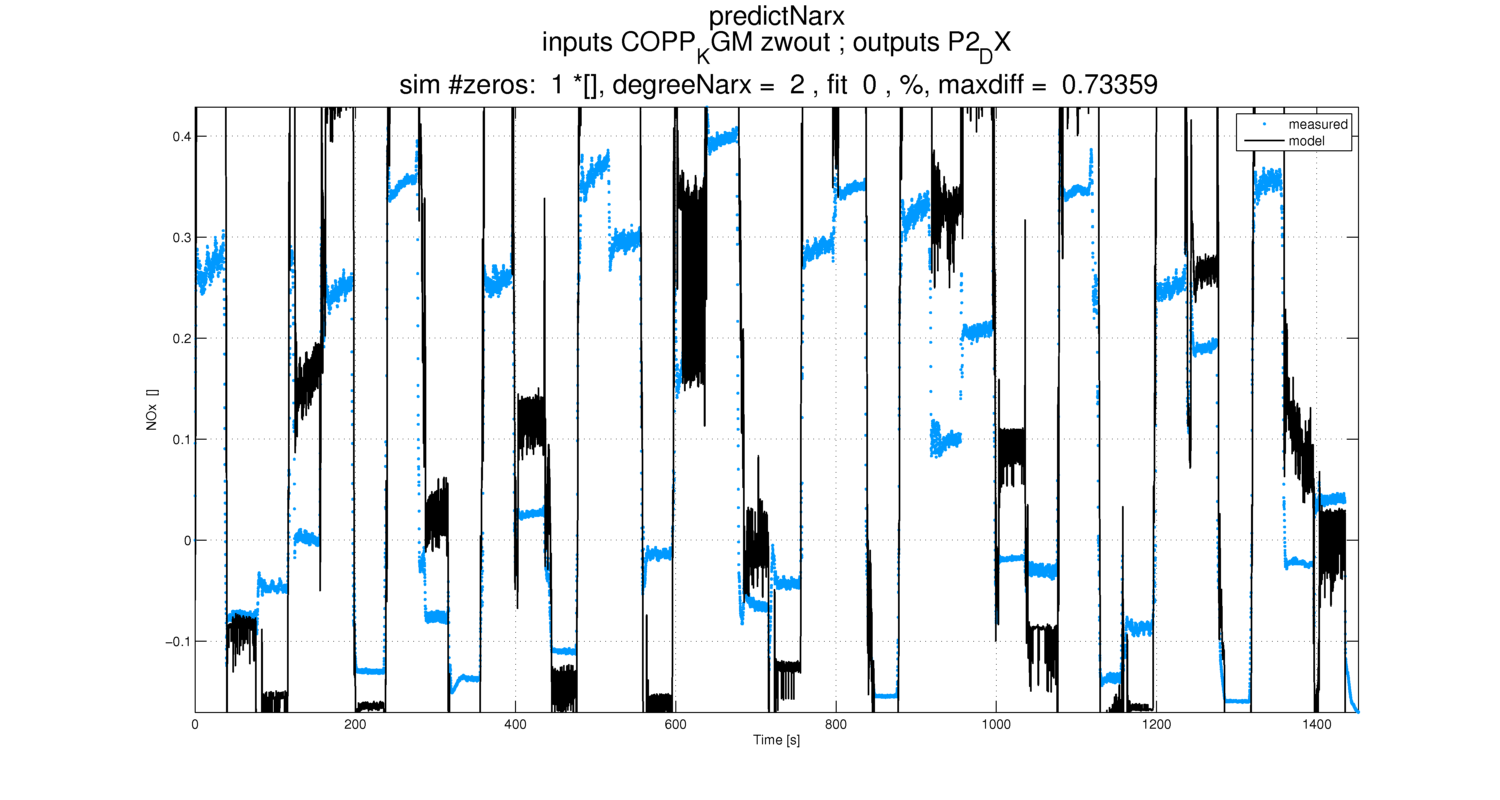
\includegraphics[width=.9\columnwidth]{Immagini/inputsCOPP_KGMzwoutoutputsP2_DX-predictNarx-3}
		\label{fig:inputsCOPP_KGMzwoutoutputsP2_DX-predictNarx-3}
	}
	\\
	\subfloat[P2 DX: Narx simulation]{
		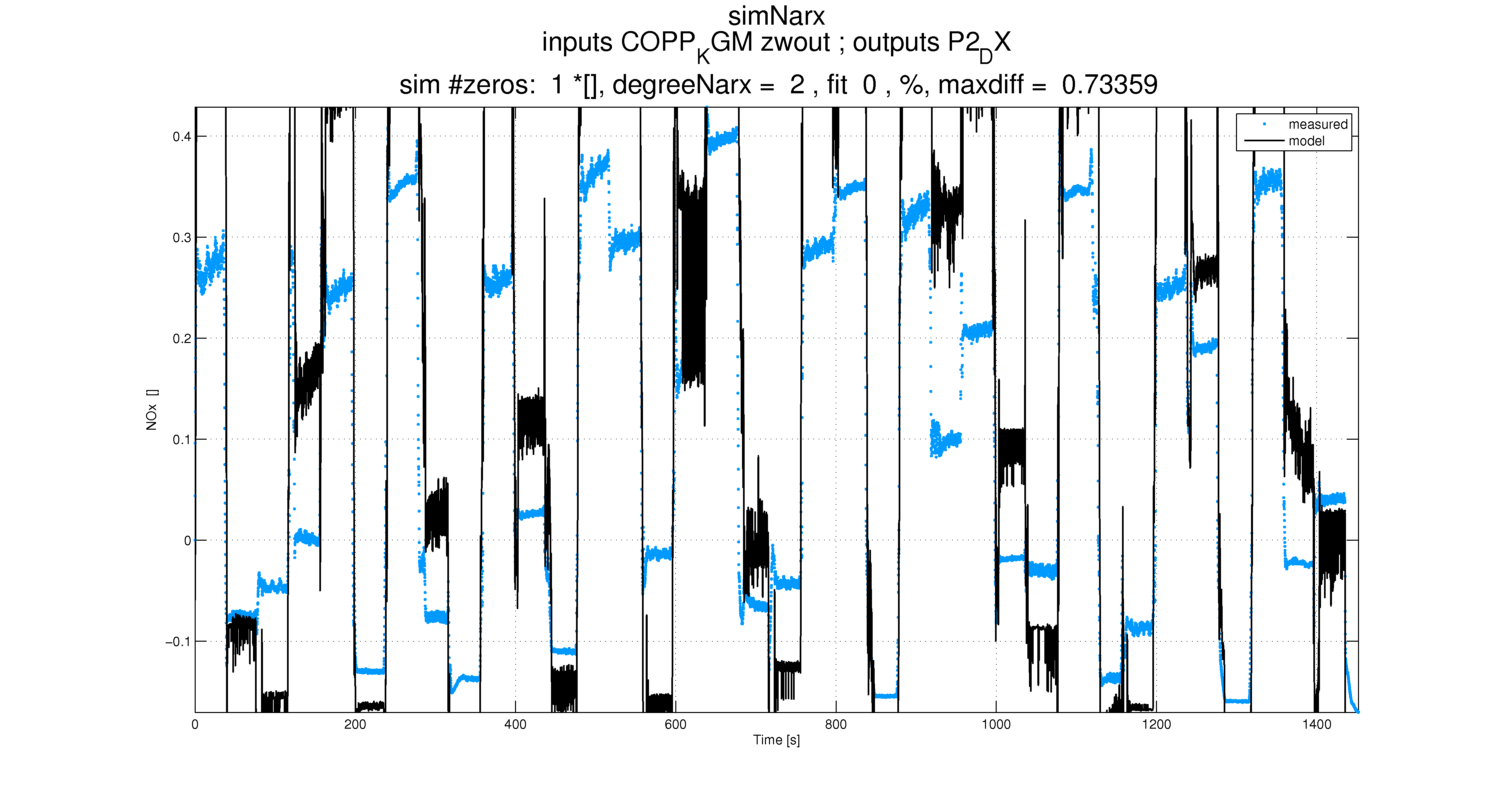
\includegraphics[width=.96\columnwidth]{Immagini/inputsCOPP_KGMzwoutoutputsP2_DX-simNarx-3}
		\label{fig:inputsCOPP_KGMzwoutoutputsP2_DX-simNarx-3}
	}
\phantomcaption	

\end{figure}


\begin{figure}[htbp] \ContinuedFloat
	\centering 
	\subfloat[P2 DX: Transfer function identification]{
		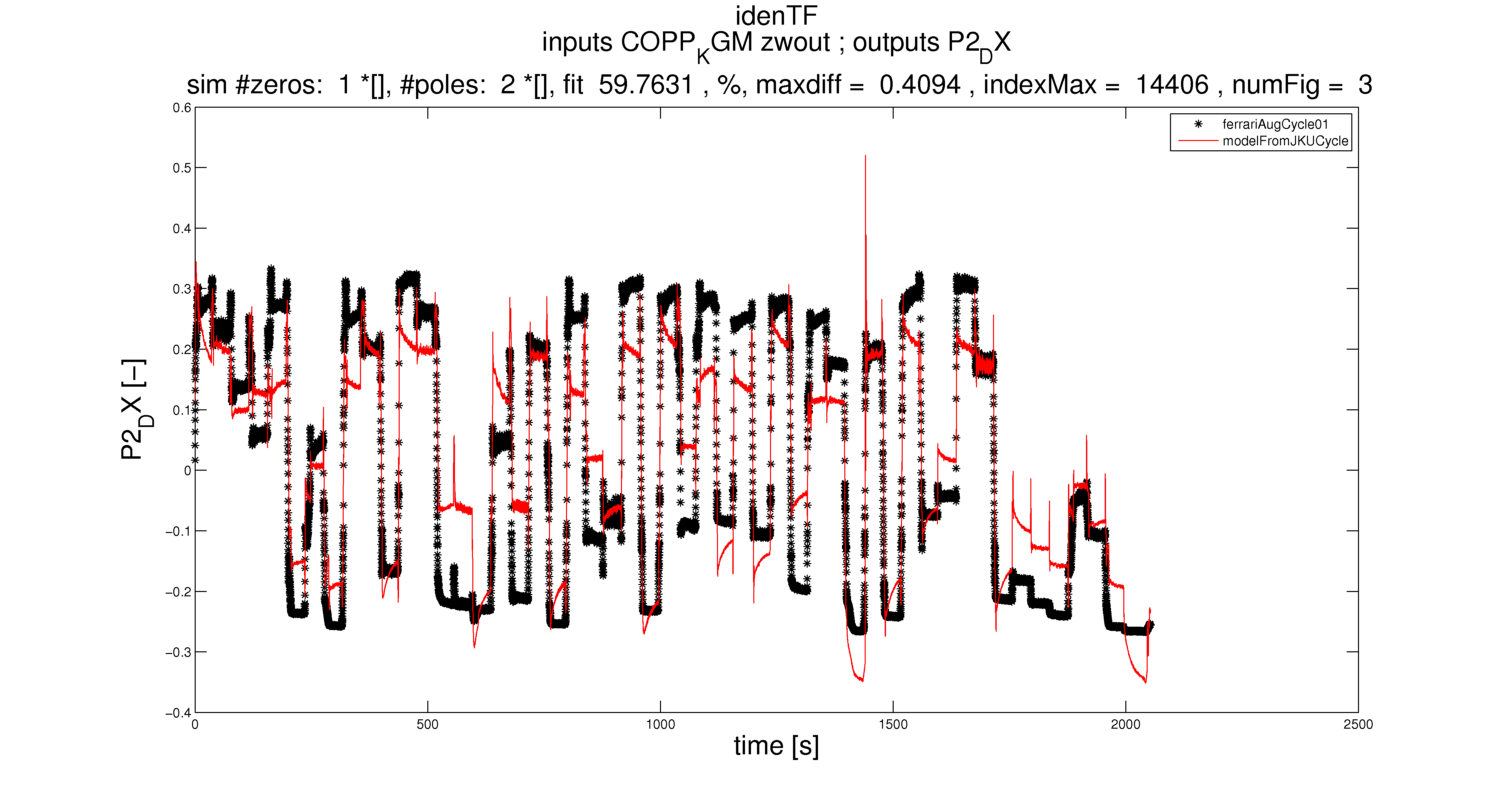
\includegraphics[width=.9\columnwidth]{Immagini/inputsCOPP_KGMzwoutoutputsP2_DX-idenTF-3}
		\label{fig:inputsCOPP_KGMzwoutoutputsP2_DX-idenTF-3}  }
	\\
	\subfloat[P2 DX: Transfer function simulation]{
		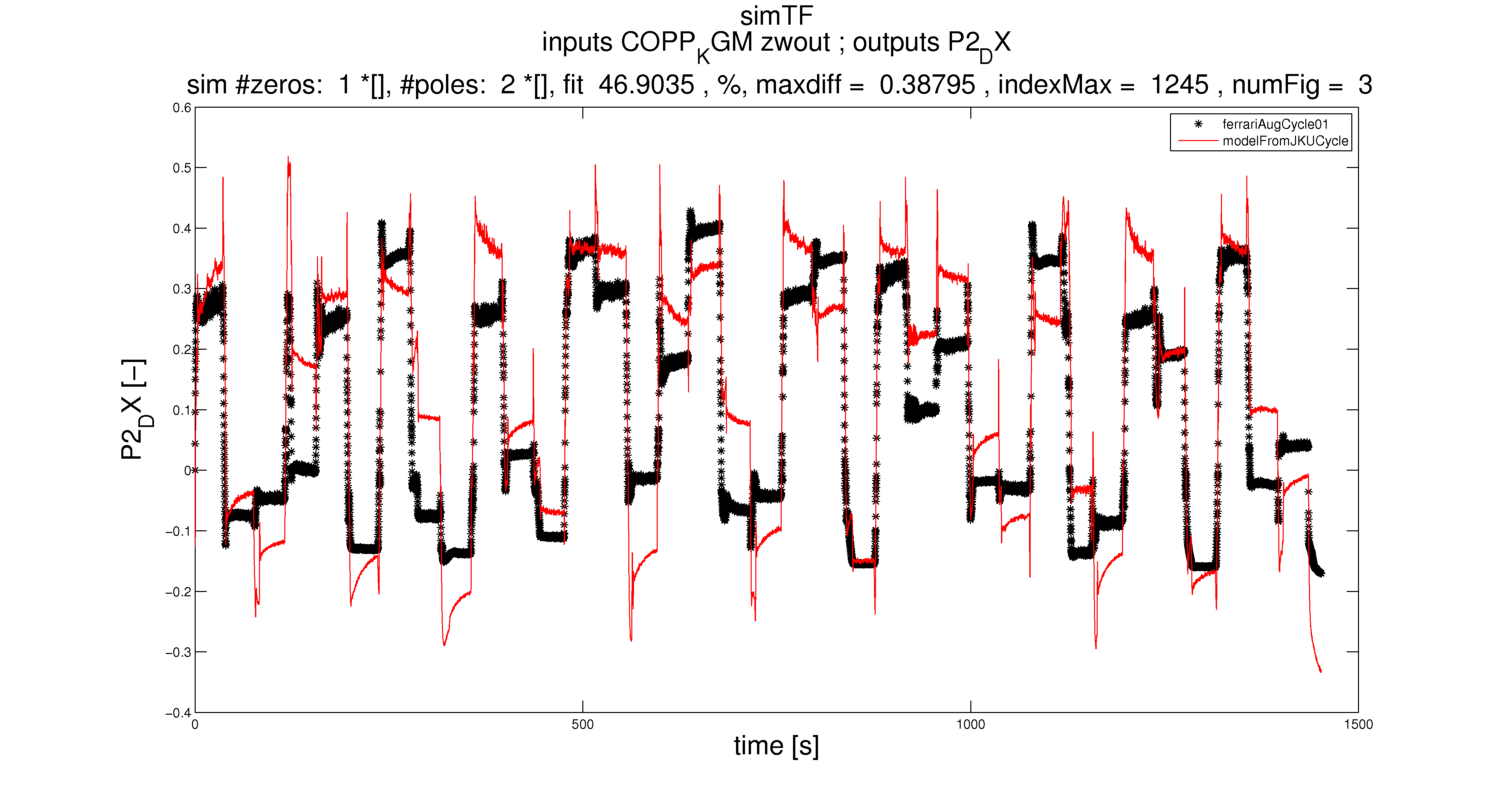
\includegraphics[width=.9\columnwidth]{Immagini/inputsCOPP_KGMzwoutoutputsP2_DX-simTF-3}
		\label{fig:inputsCOPP_KGMzwoutoutputsP2_DX-simTF-3}  }
	\\	
	\caption[Inputs: COPP KGM, zwout; Output: P2DX; np: 2; nz: 1; degree: 2]{Inputs: COPP KGM, zwout; Output: P2DX; np: 2; nz: 1; degree: 2}
	\label{fig:inputsCOPP_KGM-zwout-outputsP2_DX-3}	
\end{figure}
%%inputsCOPP_KGM-zwout-outputsP2_DX-4

\begin{figure}[htbp]
	\centering 
	\subfloat[P2 DX: Narx identification]{
		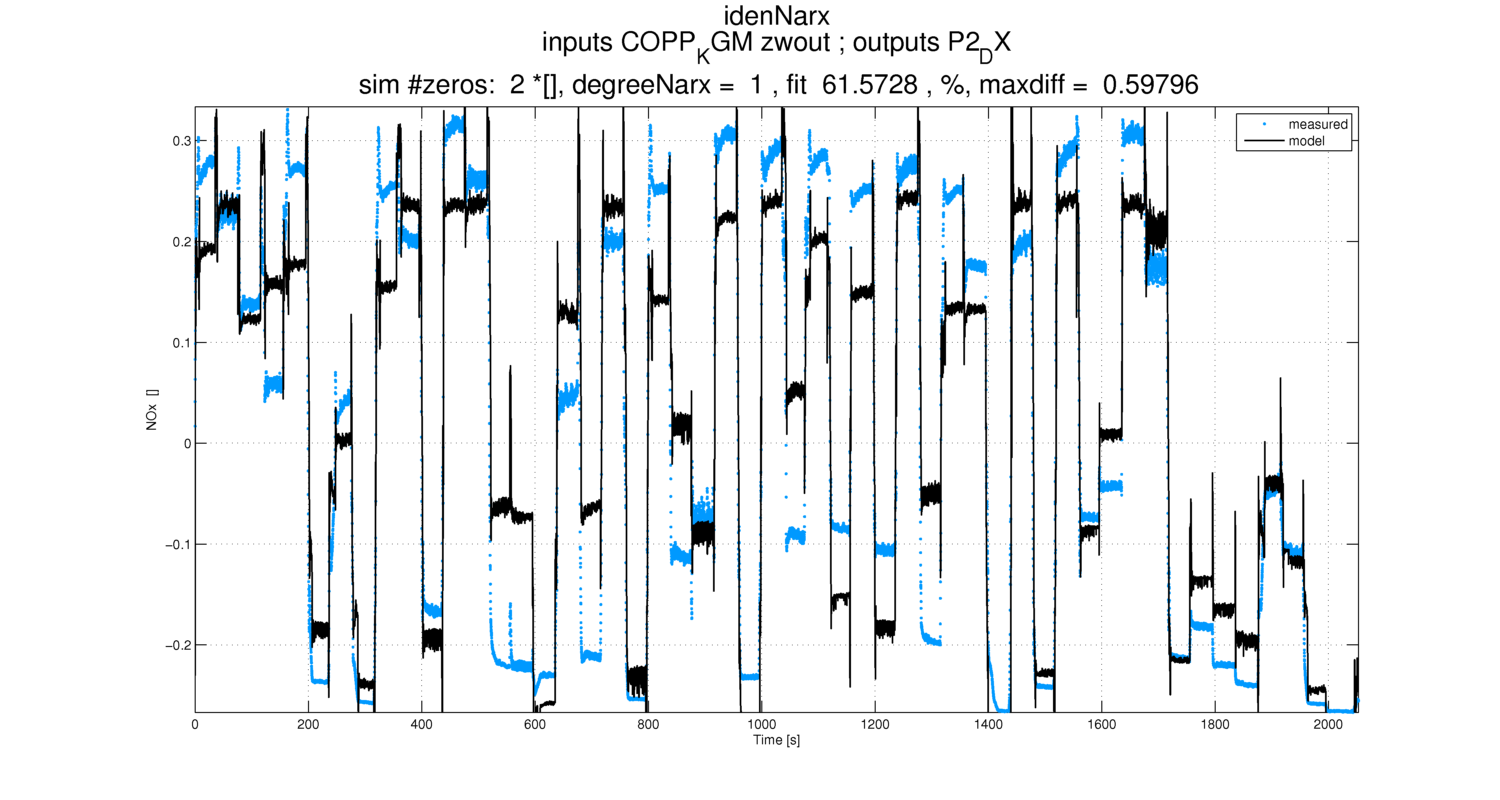
\includegraphics[width=.9\columnwidth]{Immagini/inputsCOPP_KGMzwoutoutputsP2_DX-idenNarx-4}
		\label{fig:inputsCOPP_KGMzwoutoutputsP2_DX-idenNarx-4}	}
	\\
	\subfloat[P2 DX: Narx prediction]{
		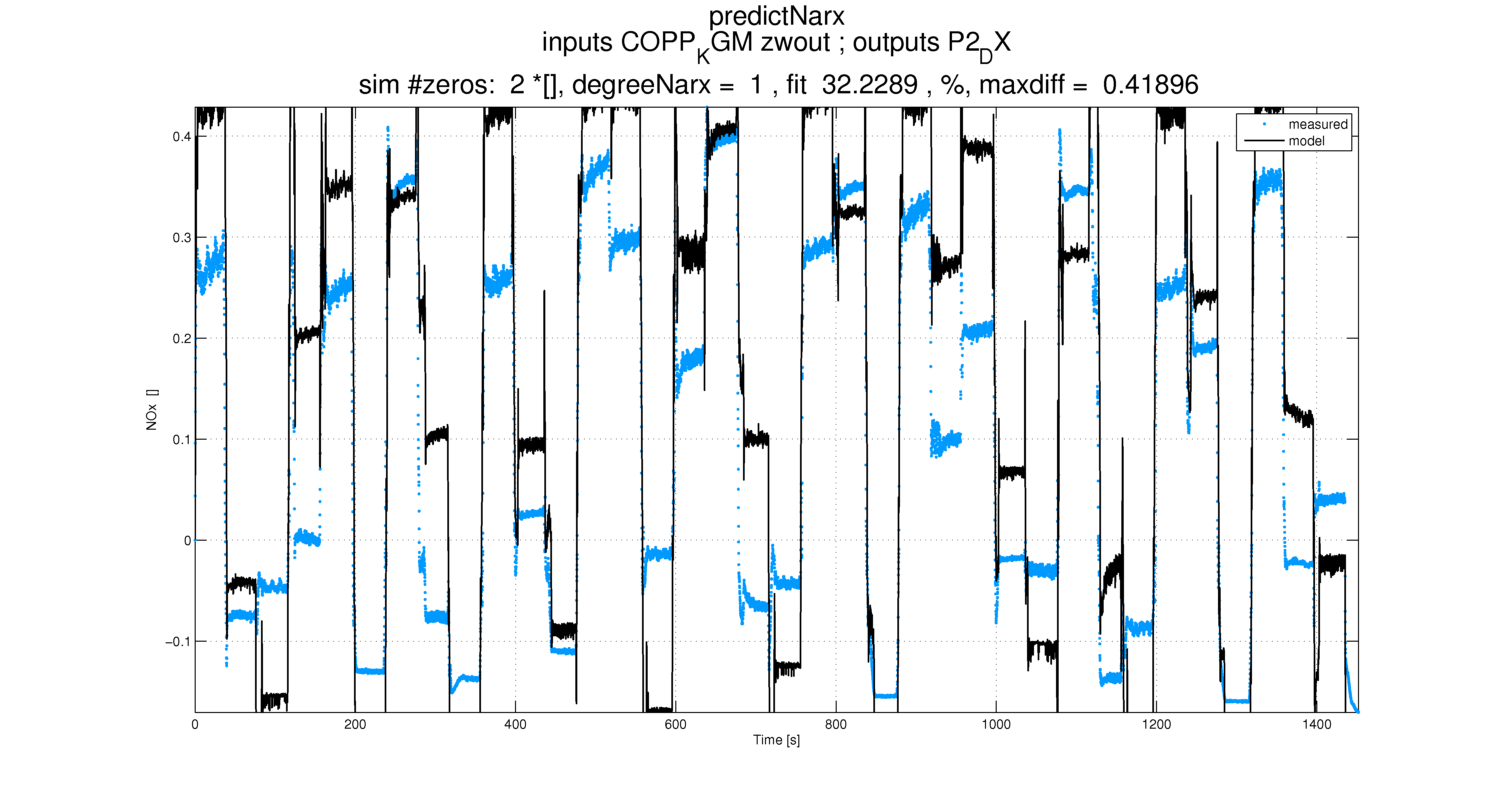
\includegraphics[width=.9\columnwidth]{Immagini/inputsCOPP_KGMzwoutoutputsP2_DX-predictNarx-4}
		\label{fig:inputsCOPP_KGMzwoutoutputsP2_DX-predictNarx-4}
	}
	\\
	\subfloat[P2 DX: Narx simulation]{
		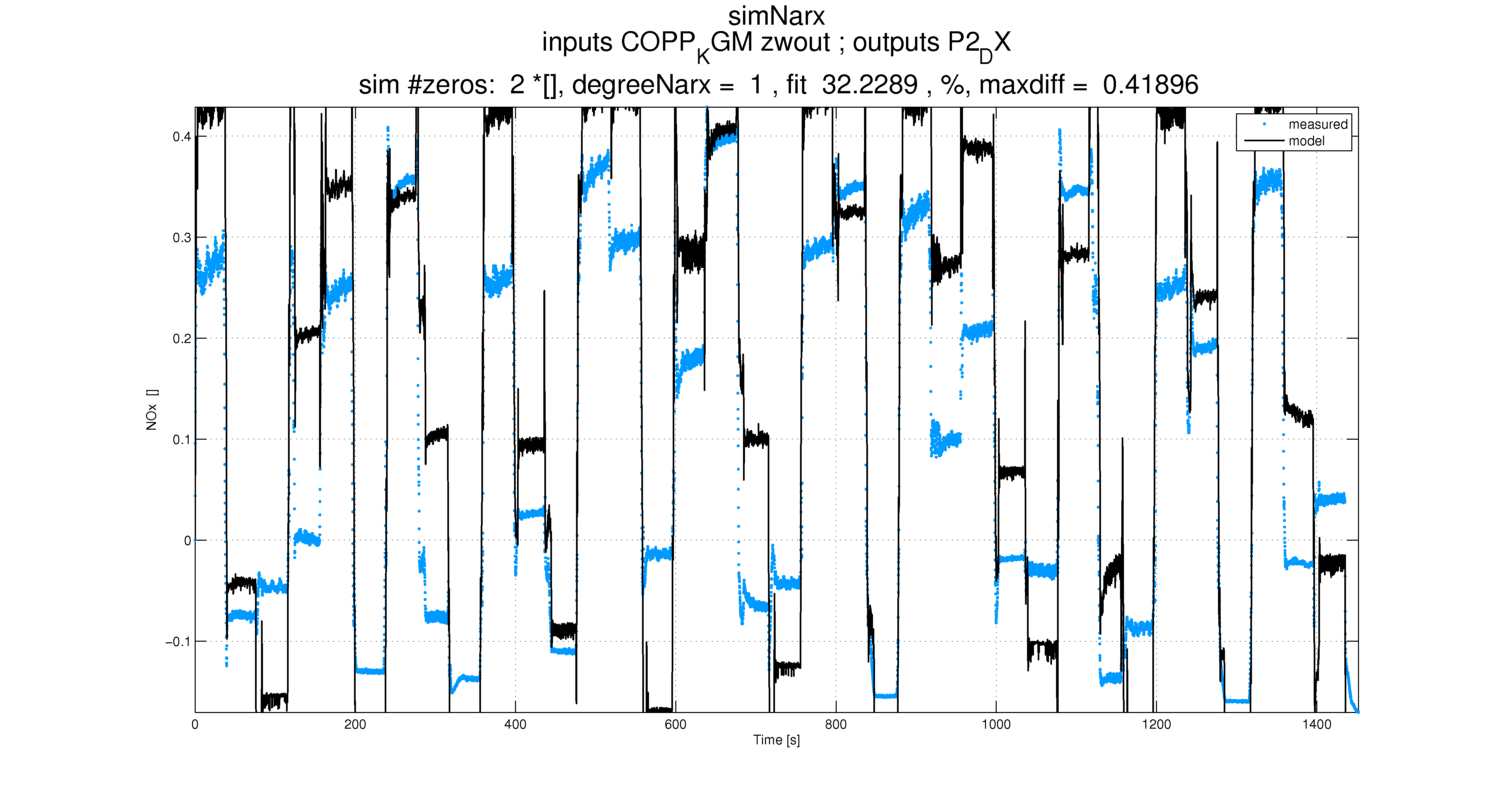
\includegraphics[width=.9\columnwidth]{Immagini/inputsCOPP_KGMzwoutoutputsP2_DX-simNarx-4}
		\label{fig:inputsCOPP_KGMzwoutoutputsP2_DX-simNarx-4}
	}
\phantomcaption
\end{figure}


\begin{figure}[htbp] \ContinuedFloat
	\centering 
	\subfloat[P2 DX: Transfer function identification]{
		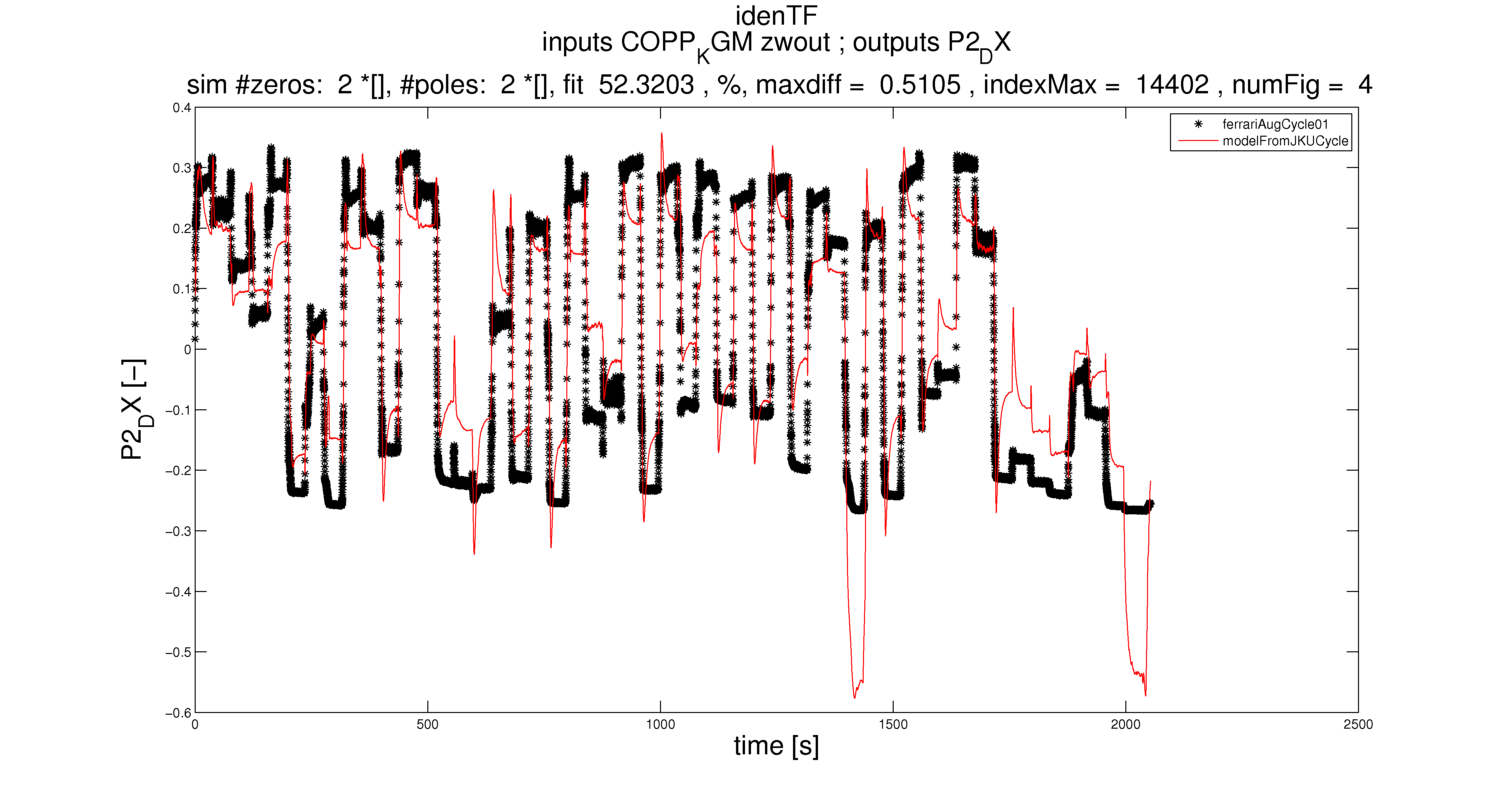
\includegraphics[width=.9\columnwidth]{Immagini/inputsCOPP_KGMzwoutoutputsP2_DX-idenTF-4}
		\label{fig:inputsCOPP_KGMzwoutoutputsP2_DX-idenTF-4}  }
	\\
	\subfloat[P2 DX: Transfer function simulation]{
		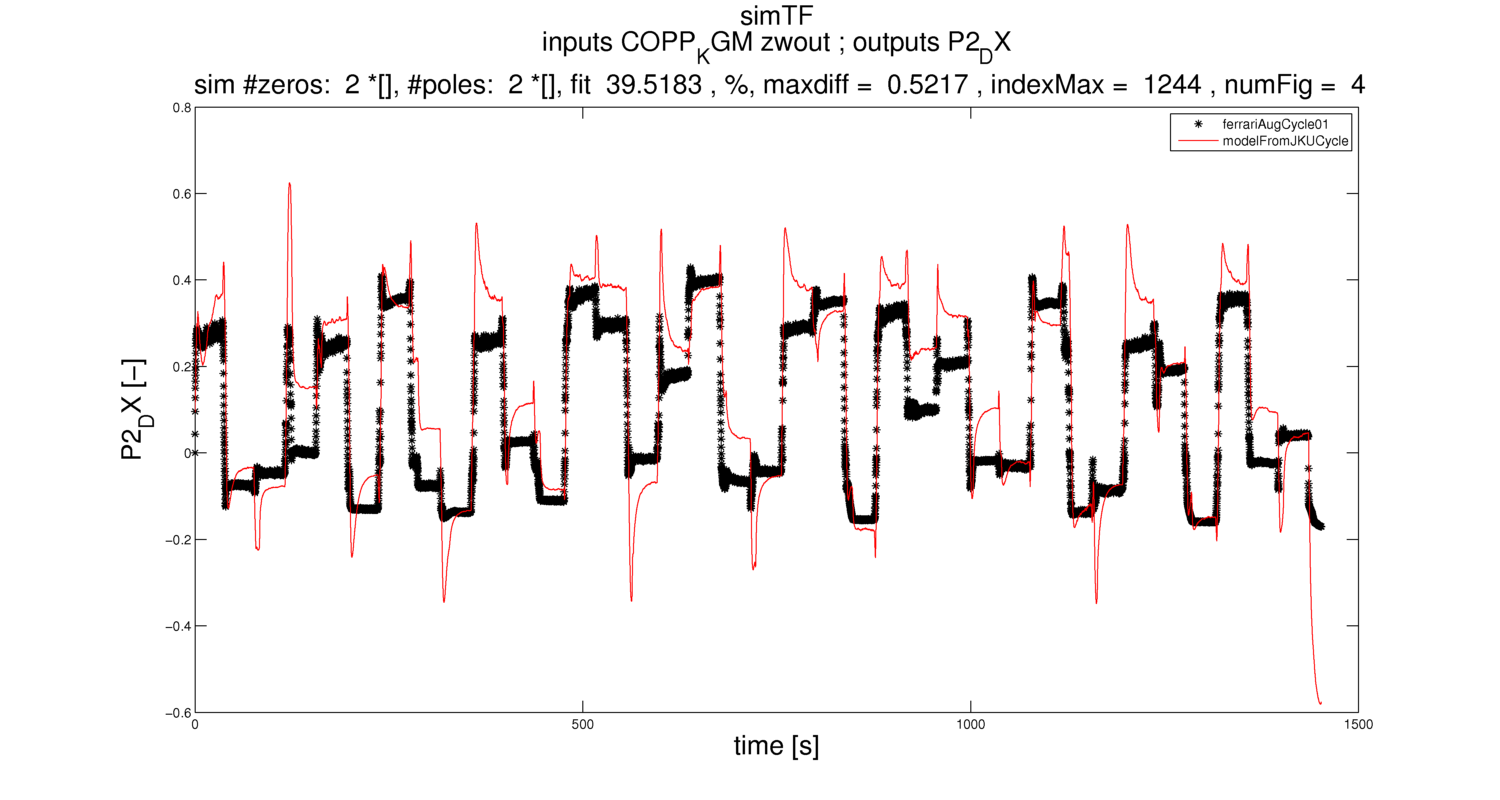
\includegraphics[width=.9\columnwidth]{Immagini/inputsCOPP_KGMzwoutoutputsP2_DX-simTF-4}
		\label{fig:inputsCOPP_KGMzwoutoutputsP2_DX-simTF-4}  }
	\\	

	\caption[Inputs: COPP KGM, zwout; Output: P2DX; np: 2; nz: 2; degree: 1]{Inputs: COPP KGM, zwout; Output: P2DX; np: 2; nz: 2; degree: 1}
	\label{fig:inputsCOPP_KGM-zwout-outputsP2_DX-4}	
\end{figure}

\newpage

\subsection{Turbocharger Right Way Out Air Pressure (P2 Dx)}
\begin{itemize}
	\item{inputs: right intake manifold pressure (p poldx), relative fuel mass right side (rk w), actual throttle pedal position (alpha i), actual engine torque (trqclth)}
	\item{output: turbocharger right way out air pressure (p2 dx)}
\end{itemize}

\begin{center} 
\begin{longtable}{ll|cccc|ccc|ccc} 
\caption[inputs P POLDX rk w ALPHA I trqCLth   outputs P2 DX]{inputs P POLDX rk w ALPHA I trqCLth   outputs P2 DX.} 
\label{tab:inputs_P_POLDX_rk_w_ALPHA_I_trqCLth___outputs_P2_DX} 
\hline 
  mdl & type & np & nz & dPl & oY & ft100 & mxDf100 & mse100 & ft200 & mxDf200 & mse200 \\ 
 \hline 
tf  & iden & 1 & 1 & 0 & 0 & 77.3 & 0.25 & 0.00 & 72.0 & 0.29 & 0.00 \\ 
tf  & sim & 1 & 1 & 0 & 0 & 71.1 & 0.27 & 0.00 & 65.4 & 0.31 & 0.00 \\ 
 \hline 
tf  & iden & 1 & 2 & 0 & 0 & 77.8 & 0.25 & 0.00 & 73.9 & 0.28 & 0.00 \\ 
tf  & sim & 1 & 2 & 0 & 0 & 71.7 & 0.26 & 0.00 & 67.5 & 0.29 & 0.00 \\ 
 \hline 
tf  & iden & 2 & 1 & 0 & 0 & 77.5 & 0.25 & 0.00 & 72.6 & 0.29 & 0.00 \\ 
tf  & sim & 2 & 1 & 0 & 0 & 71.6 & 0.27 & 0.00 & 66.4 & 0.30 & 0.00 \\ 
 \hline 
tf  & iden & 2 & 2 & 0 & 0 & 78.2 & 0.25 & 0.00 & 72.0 & 0.28 & 0.00 \\ 
tf  & sim & 2 & 2 & 0 & 0 & 68.7 & 0.25 & 0.00 & 65.7 & 0.29 & 0.00 \\ 
 \hline 
narx & iden & 0 & 1 & 1 & 1 & 88.4 & 0.18 & 0.00 & 84.1 & 0.18 & 0.00 \\ 
narx & pred & 0 & 1 & 1 & 1 & 84.3 & 0.23 & 0.03 & 79.5 & 0.15 & 0.04 \\ 
narx & sim & 0 & 1 & 1 & 1 & 61.6 & 0.28 & 0.07 & 69.0 & 0.18 & 0.06 \\ 
 \hline 
narx & iden & 0 & 1 & 1 & 2 & 89.6 & 0.21 & 0.00 & 84.6 & 0.21 & 0.00 \\ 
narx & pred & 0 & 1 & 1 & 2 & 85.5 & 0.28 & 0.03 & 80.3 & 0.16 & 0.04 \\ 
narx & sim & 0 & 1 & 1 & 2 & 62.2 & 0.25 & 0.07 & 69.4 & 0.16 & 0.06 \\ 
 \hline 
narx & iden & 0 & 1 & 1 & 3 & 89.6 & 0.21 & 0.00 & 84.6 & 0.21 & 0.00 \\ 
narx & pred & 0 & 1 & 1 & 3 & 85.5 & 0.28 & 0.03 & 80.3 & 0.16 & 0.04 \\ 
narx & sim & 0 & 1 & 1 & 3 & 62.2 & 0.25 & 0.07 & 69.4 & 0.16 & 0.06 \\ 
 \hline 
\end{longtable} 
\end{center}

%%inputsP_POLDXrk_wALPHA_ItrqCLthoutputsP2_DX-1.tex

\begin{figure}[htbp]
	\centering 
	\subfloat[P2 DX: Narx identification]{
		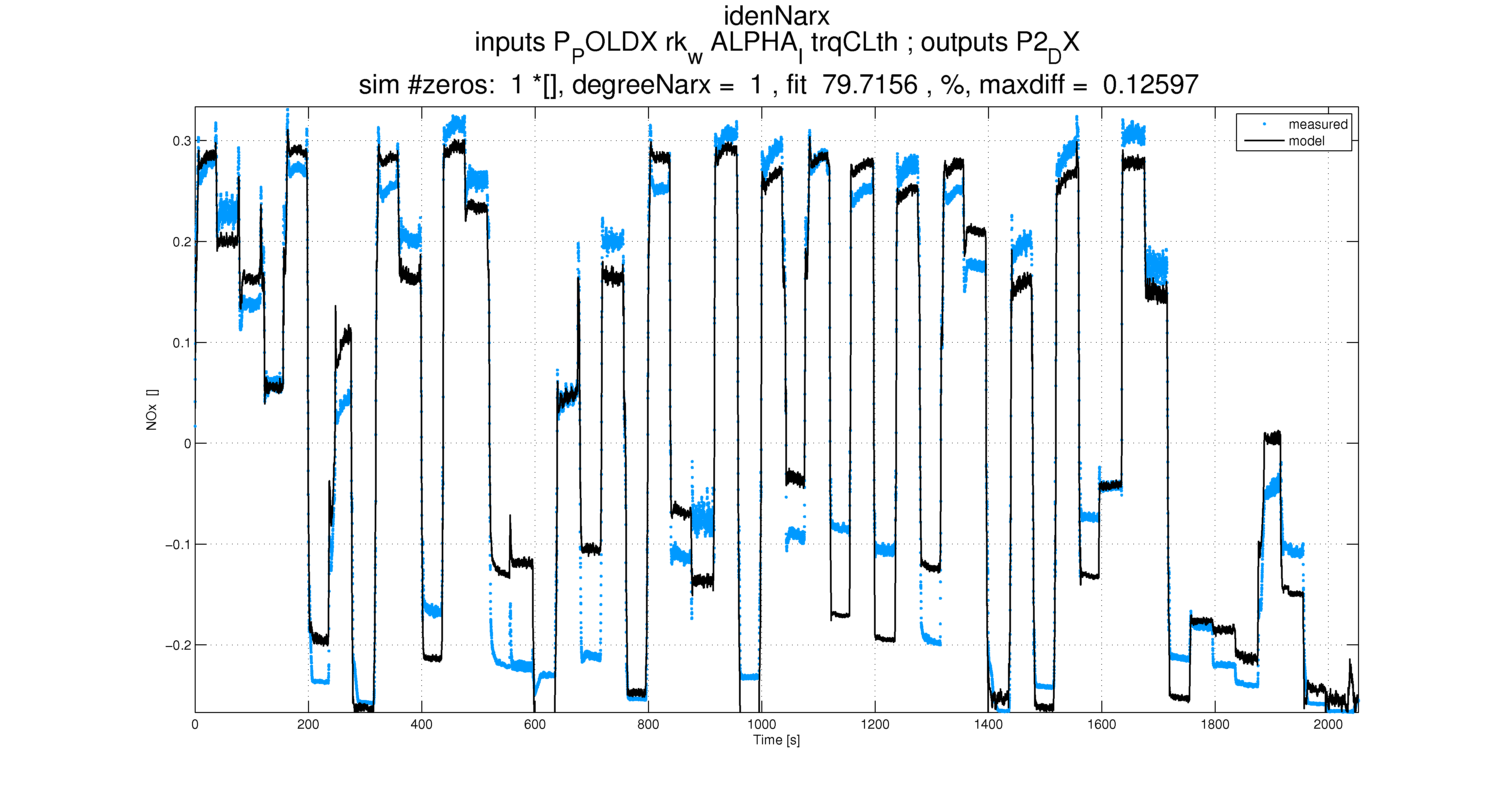
\includegraphics[width=.9\columnwidth]{Immagini/inputsP_POLDXrk_wALPHA_ItrqCLthoutputsP2_DX-idenNarx-1}
		\label{fig:inputsP_POLDXrk_wALPHA_ItrqCLthoutputsP2_DX-idenNarx-1}	}
	\\
	\subfloat[P2 DX: Narx prediction]{
		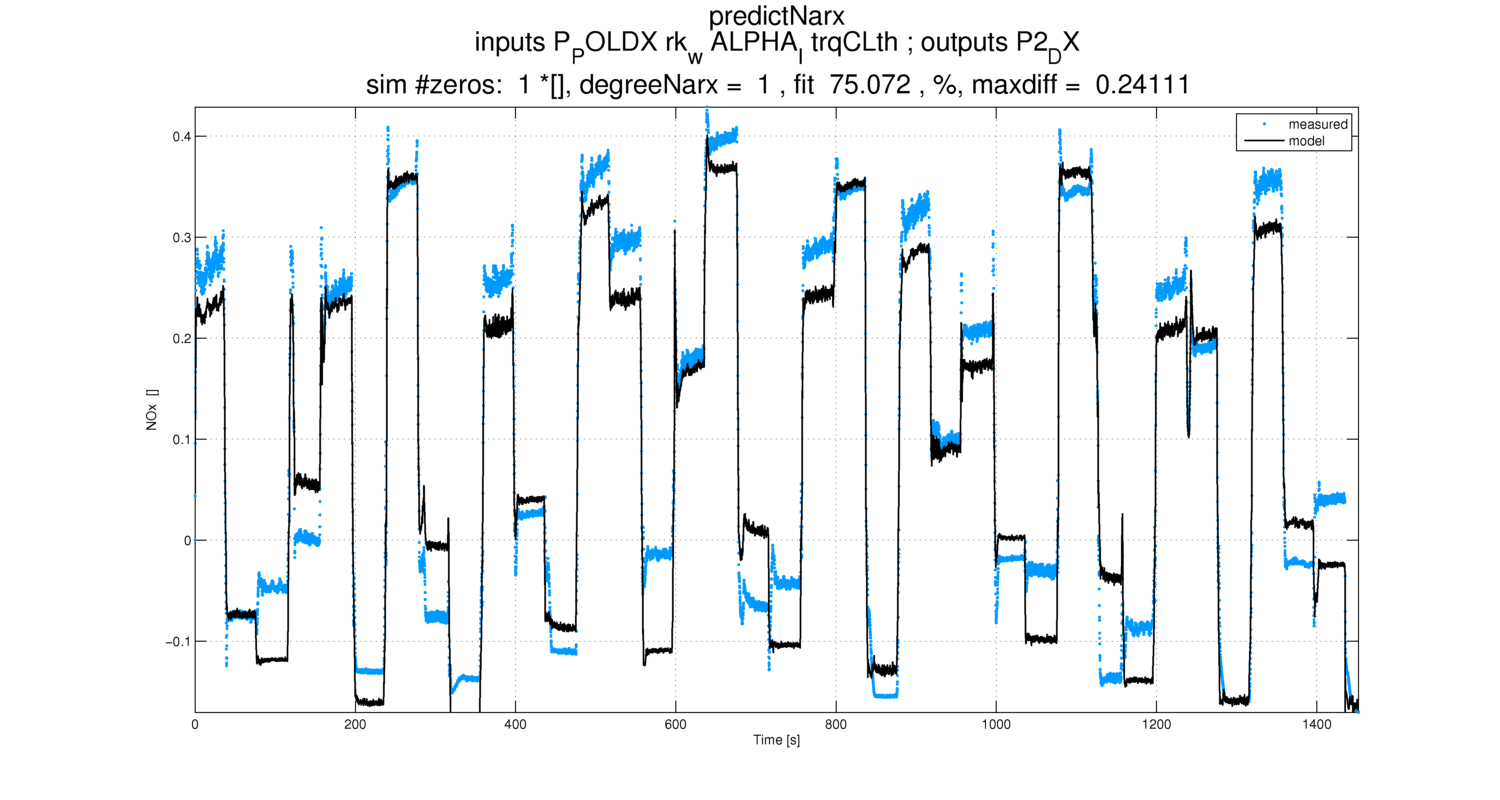
\includegraphics[width=.9\columnwidth]{Immagini/inputsP_POLDXrk_wALPHA_ItrqCLthoutputsP2_DX-predictNarx-1}
		\label{fig:inputsP_POLDXrk_wALPHA_ItrqCLthoutputsP2_DX-predictNarx-1}
	}
	\\
	\subfloat[P2 DX: Narx simulation]{
		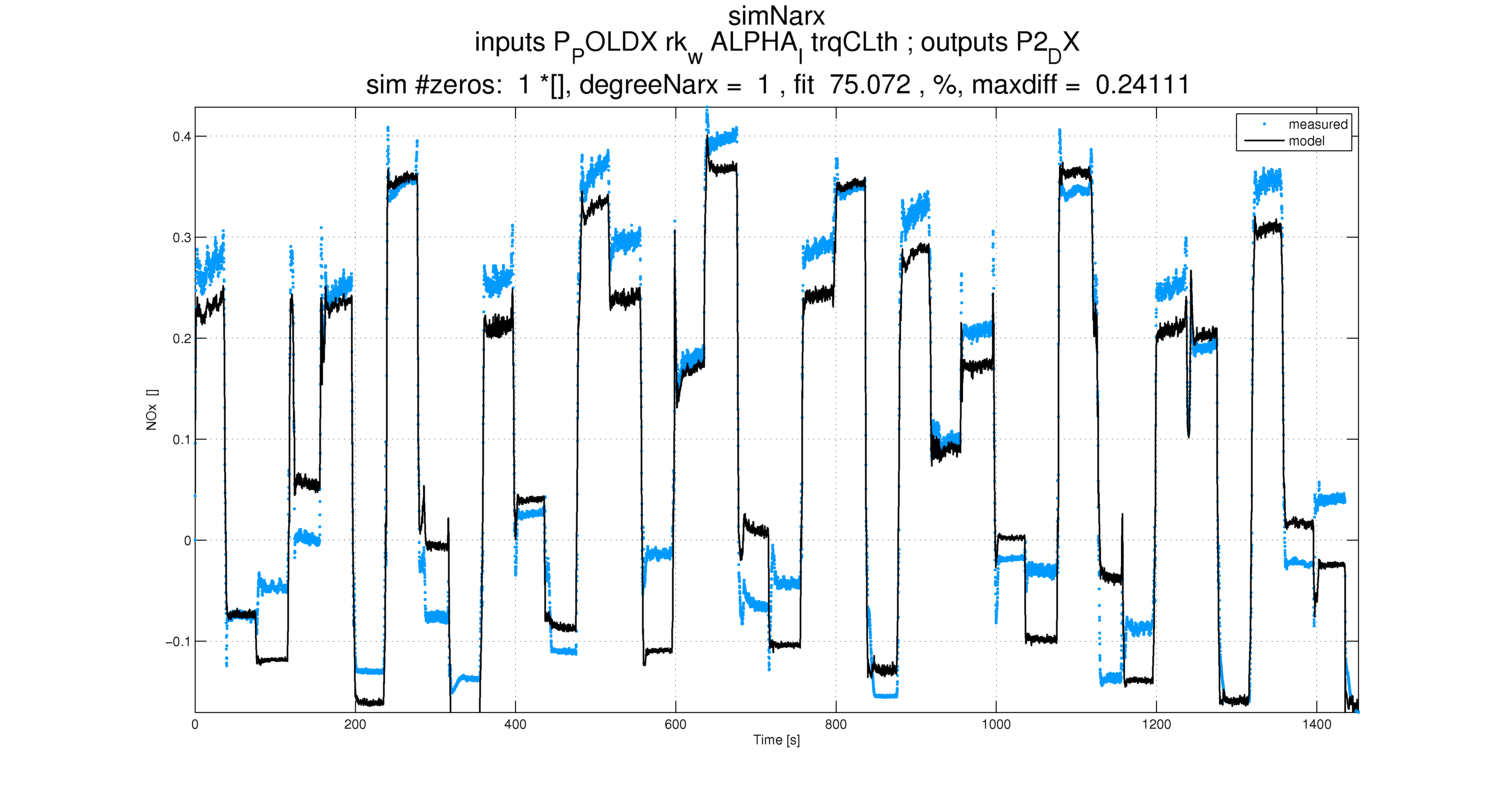
\includegraphics[width=.9\columnwidth]{Immagini/inputsP_POLDXrk_wALPHA_ItrqCLthoutputsP2_DX-simNarx-1}
		\label{fig:inputsP_POLDXrk_wALPHA_ItrqCLthoutputsP2_DX-simNarx-1}
	}
\phantomcaption
\end{figure}


\begin{figure}[htbp] \ContinuedFloat
	\centering 
	\subfloat[P2 DX: Transfer function identification]{
		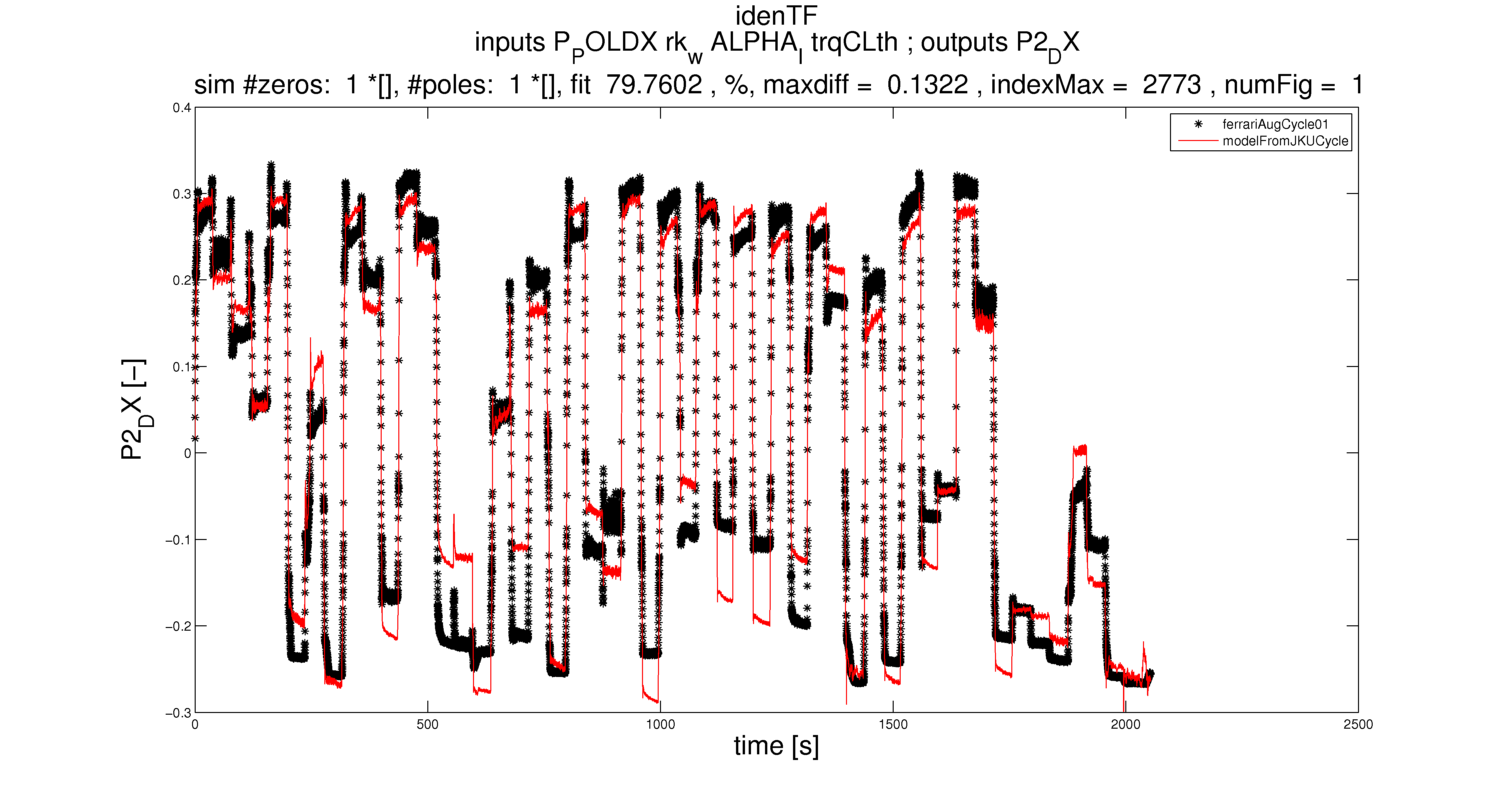
\includegraphics[width=.9\columnwidth]{Immagini/inputsP_POLDXrk_wALPHA_ItrqCLthoutputsP2_DX-idenTF-1}
		\label{fig:inputsP_POLDXrk_wALPHA_ItrqCLthoutputsP2_DX-idenTF-1}  }
	\\
	\subfloat[P2 DX: Transfer function simulation]{
		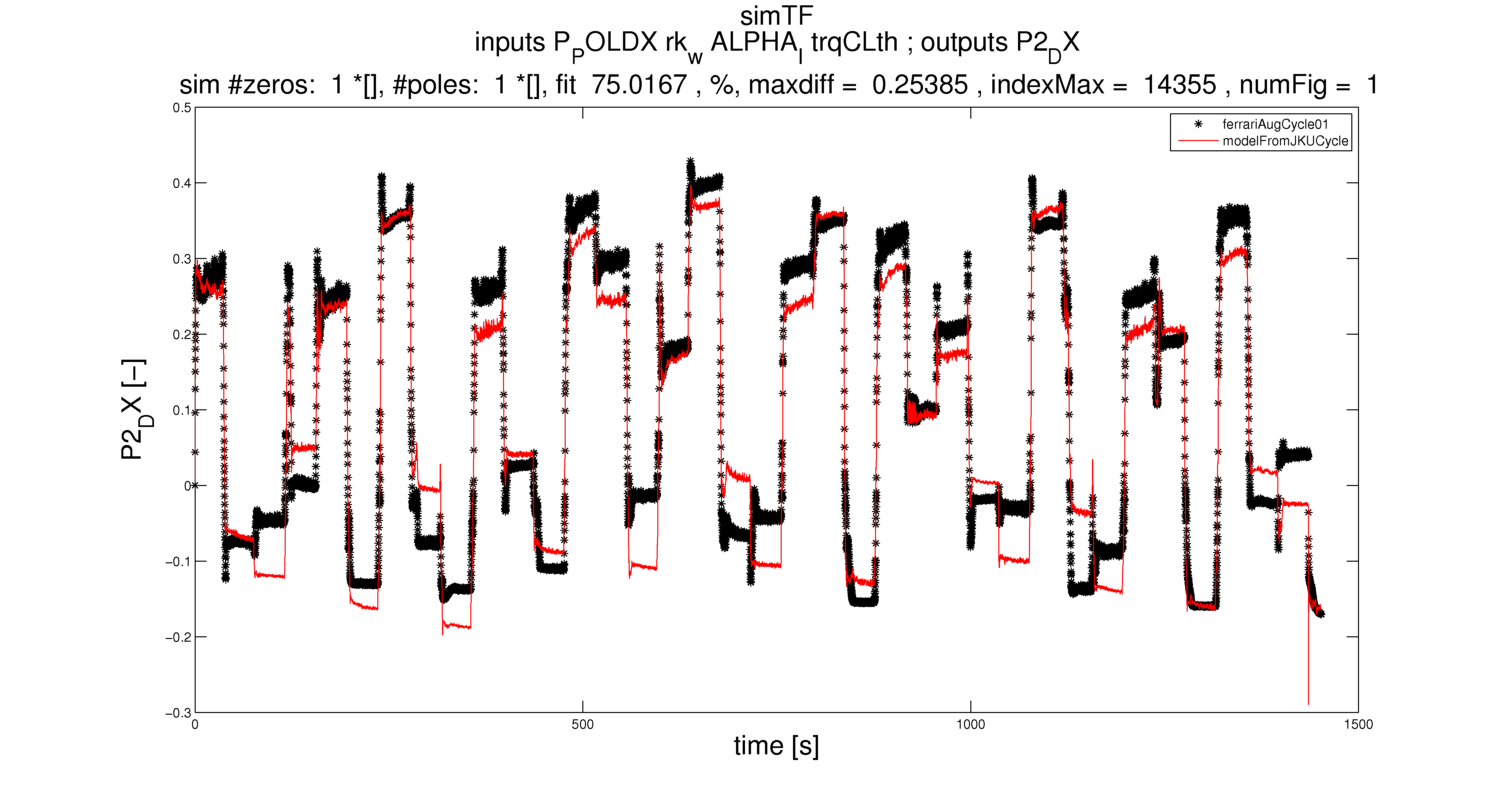
\includegraphics[width=.9\columnwidth]{Immagini/inputsP_POLDXrk_wALPHA_ItrqCLthoutputsP2_DX-simTF-1}
		\label{fig:inputsP_POLDXrk_wALPHA_ItrqCLthoutputsP2_DX-simTF-1}  }
	\\	
	\caption[Inputs: P POLDX, rk w, ALPHA I, trqCLth; Output: P2DX; np: 1; nz: 1; degree: 1]{Inputs: P POLDX, rk w, ALPHA I, trqCLth; Output: P2DX; np: 1; nz: 1; degree: 1}
	\label{fig:inputsP_POLDXrk_wALPHA_ItrqCLthoutputsP2_DX-1}
\end{figure}
%%inputsP_POLDXrk_wALPHA_ItrqCLthoutputsP2_DX-2.tex

\begin{figure}[htbp]
	\centering 
	\subfloat[P2 DX: Narx identification]{
		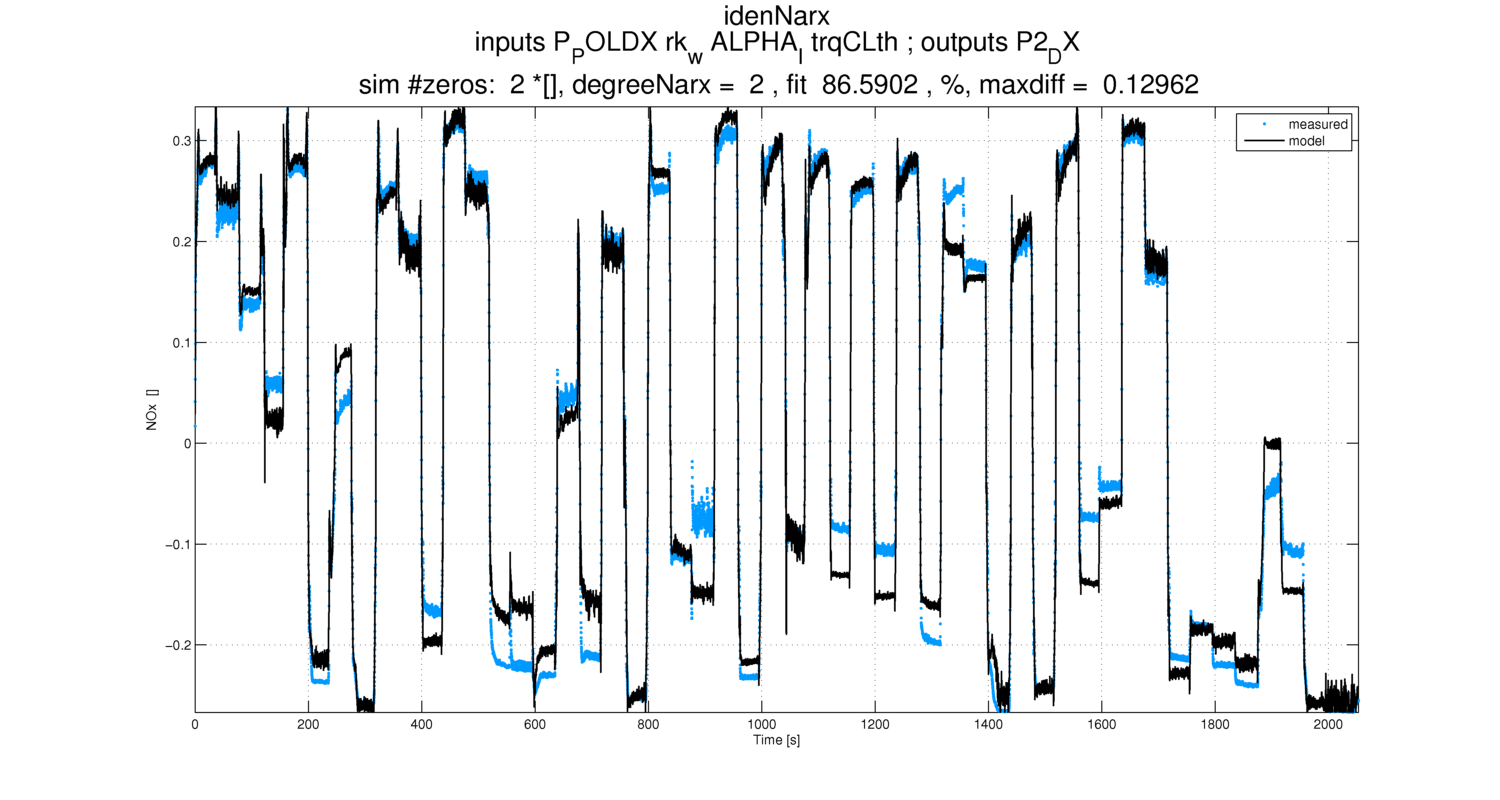
\includegraphics[width=.9\columnwidth]{Immagini/inputsP_POLDXrk_wALPHA_ItrqCLthoutputsP2_DX-idenNarx-2}
		\label{fig:inputsP_POLDXrk_wALPHA_ItrqCLthoutputsP2_DX-idenNarx-2}	}
	\\
	\subfloat[P2 DX: Narx prediction]{
		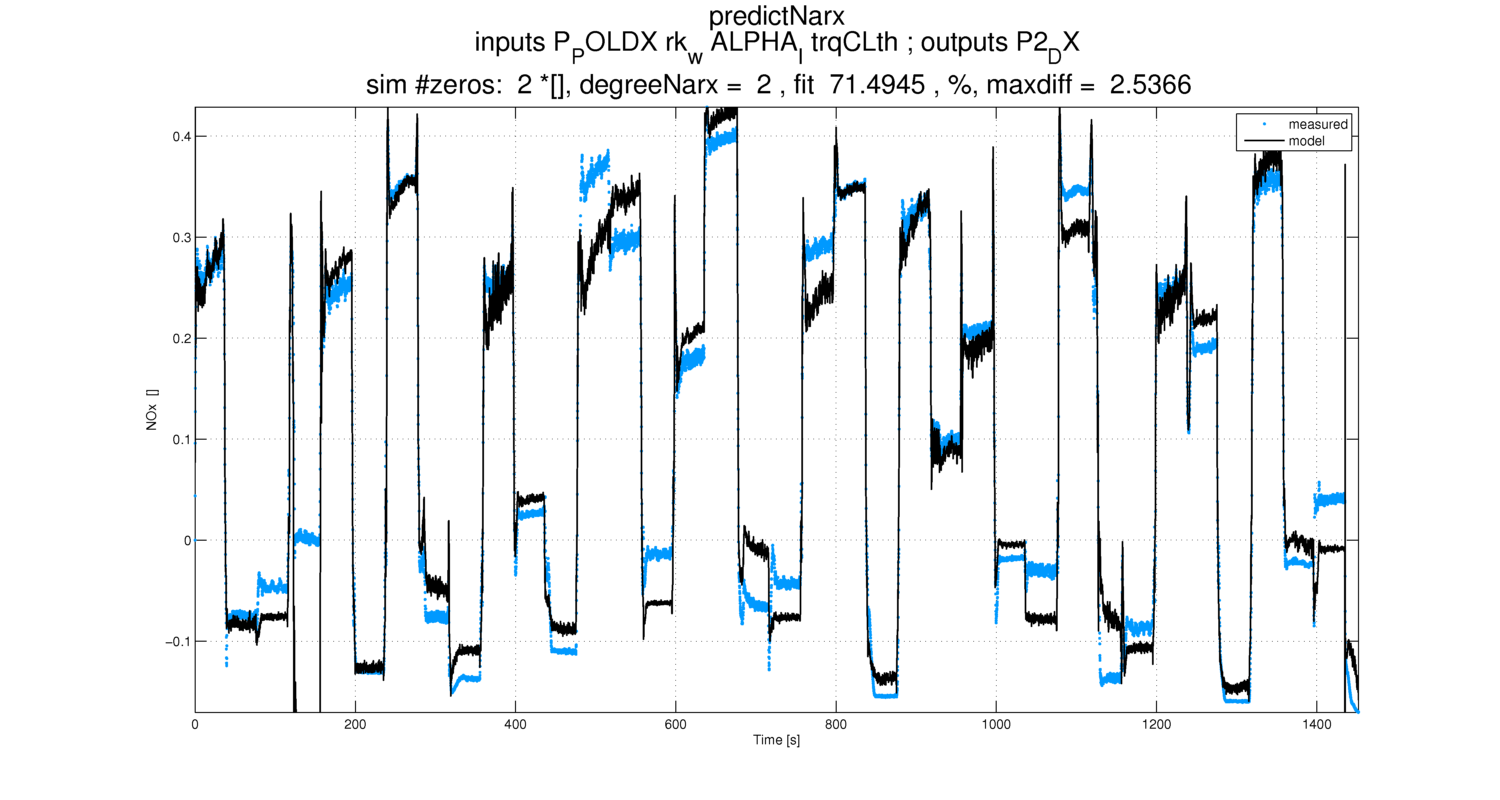
\includegraphics[width=.9\columnwidth]{Immagini/inputsP_POLDXrk_wALPHA_ItrqCLthoutputsP2_DX-predictNarx-2}
		\label{fig:inputsP_POLDXrk_wALPHA_ItrqCLthoutputsP2_DX-predictNarx-2}
	}
	\\
	\subfloat[P2 DX: Narx simulation]{
		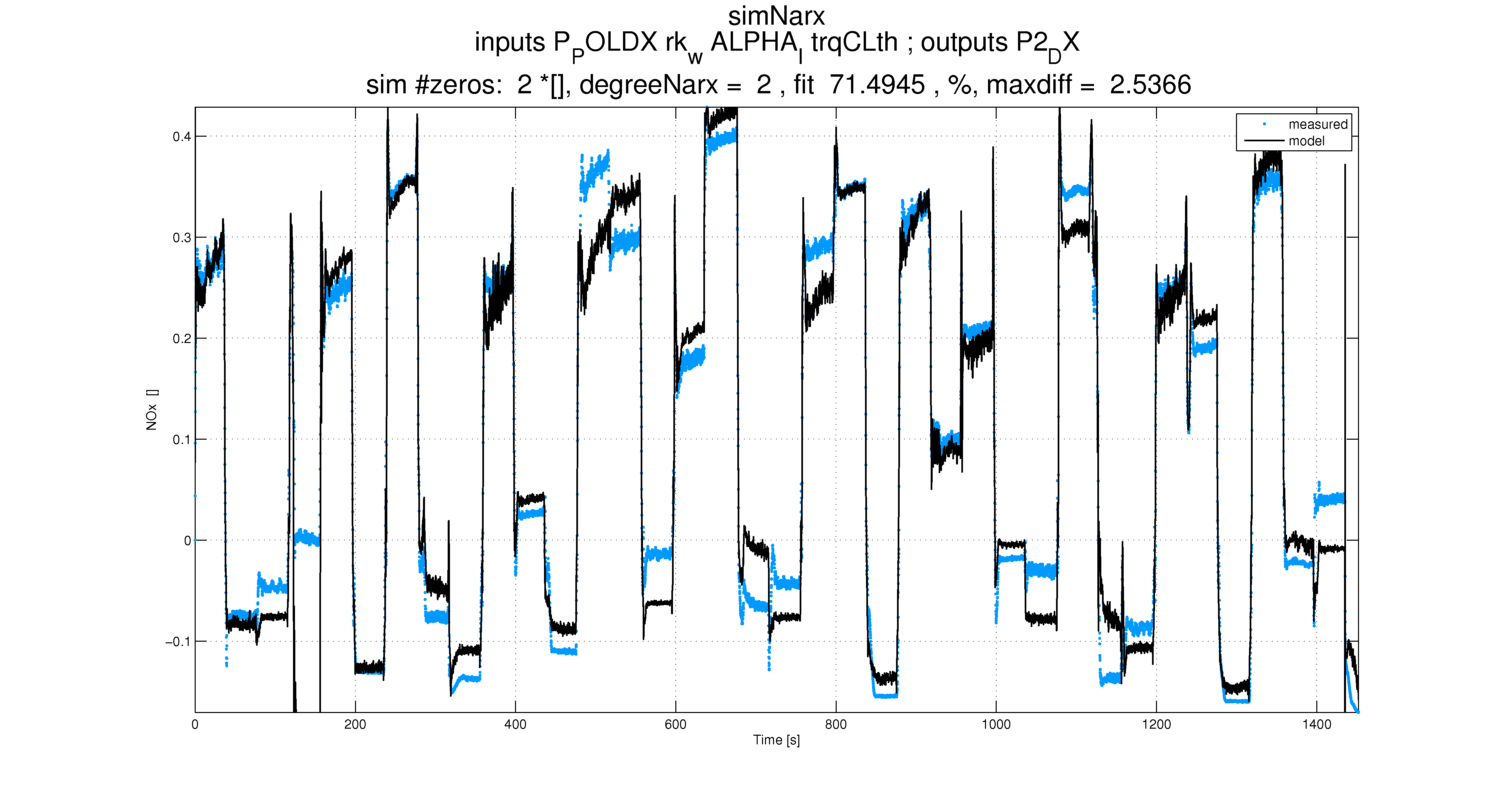
\includegraphics[width=.9\columnwidth]{Immagini/inputsP_POLDXrk_wALPHA_ItrqCLthoutputsP2_DX-simNarx-2}
		\label{fig:inputsP_POLDXrk_wALPHA_ItrqCLthoutputsP2_DX-simNarx-2}
	}
\phantomcaption
\end{figure}


\begin{figure}[htbp] \ContinuedFloat
	\centering 
	\subfloat[P2 DX: Transfer function identification]{
		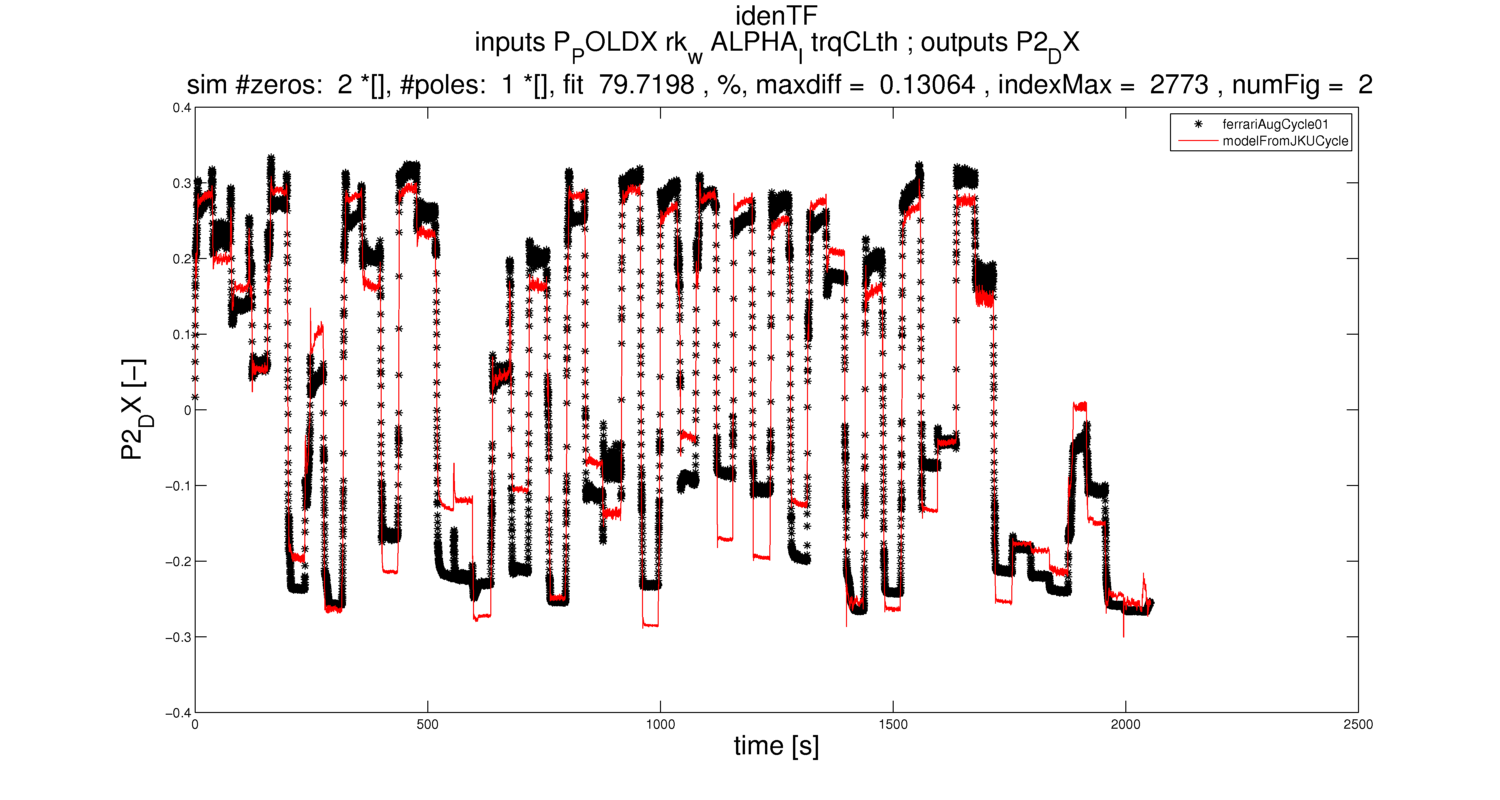
\includegraphics[width=.9\columnwidth]{Immagini/inputsP_POLDXrk_wALPHA_ItrqCLthoutputsP2_DX-idenTF-2}
		\label{fig:inputsP_POLDXrk_wALPHA_ItrqCLthoutputsP2_DX-idenTF-2}  }
	\\
	\subfloat[P2 DX: Transfer function simulation]{
		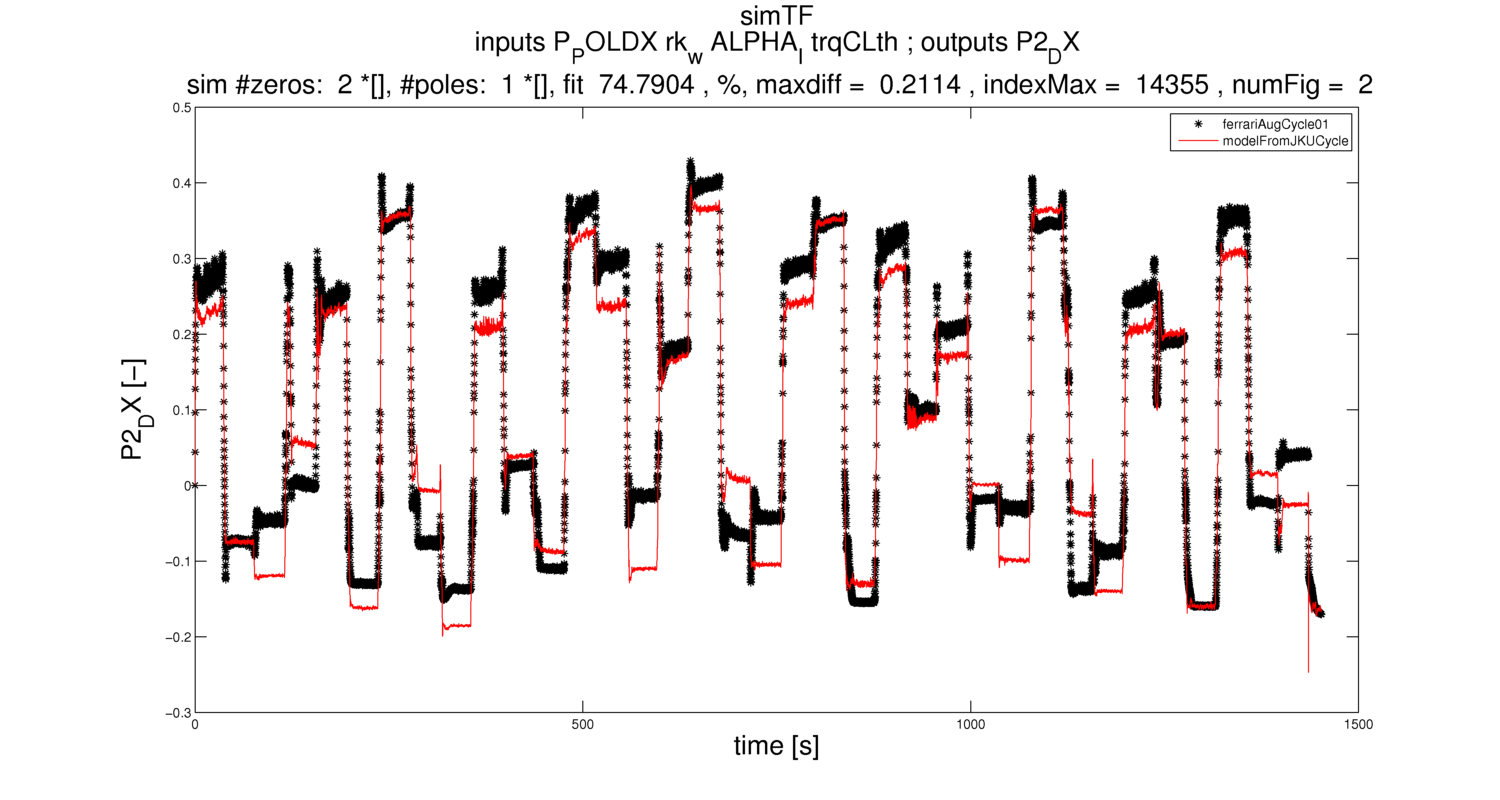
\includegraphics[width=.9\columnwidth]{Immagini/inputsP_POLDXrk_wALPHA_ItrqCLthoutputsP2_DX-simTF-2}
		\label{fig:inputsP_POLDXrk_wALPHA_ItrqCLthoutputsP2_DX-simTF-2}  }
	\\	
	\caption[Inputs: P POLDX, rk w, ALPHA I, trqCLth; Output: P2DX; np: 1; nz: 2; degree: 2]{Inputs: P POLDX, rk w, ALPHA I, trqCLth; Output: P2DX; np: 1; nz: 2; degree: 2}
	\label{fig:inputsP_POLDXrk_wALPHA_ItrqCLthoutputsP2_DX-2}
\end{figure}
%%inputsP_POLDXrk_wALPHA_ItrqCLthoutputsP2_DX-3.tex

\begin{figure}[htbp]
	\centering 
	\subfloat[P2 DX: Narx identification]{
		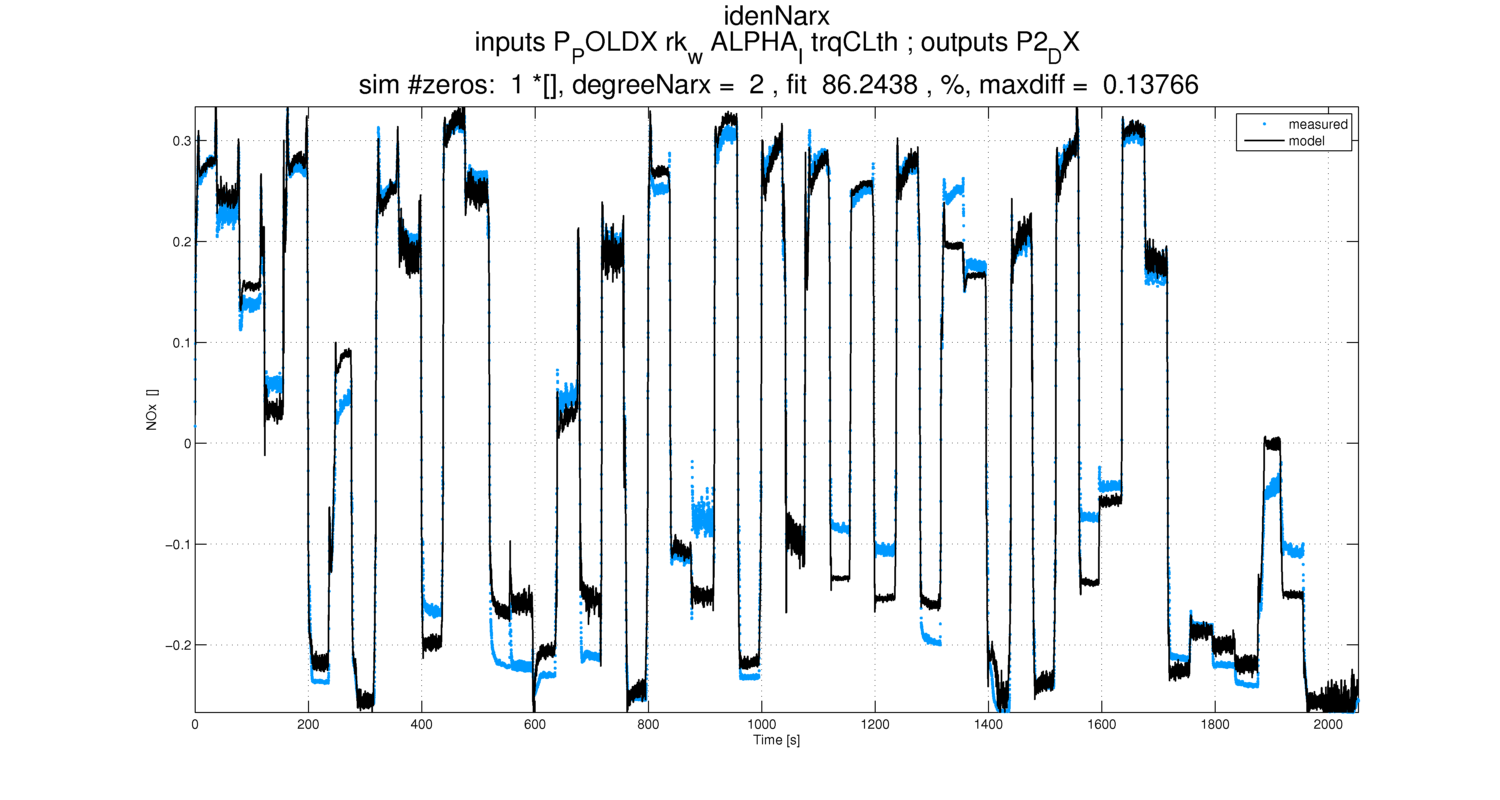
\includegraphics[width=.9\columnwidth]{Immagini/inputsP_POLDXrk_wALPHA_ItrqCLthoutputsP2_DX-idenNarx-3}
		\label{fig:inputsP_POLDXrk_wALPHA_ItrqCLthoutputsP2_DX-idenNarx-3}	}
	\\
	\subfloat[P2 DX: Narx prediction]{
		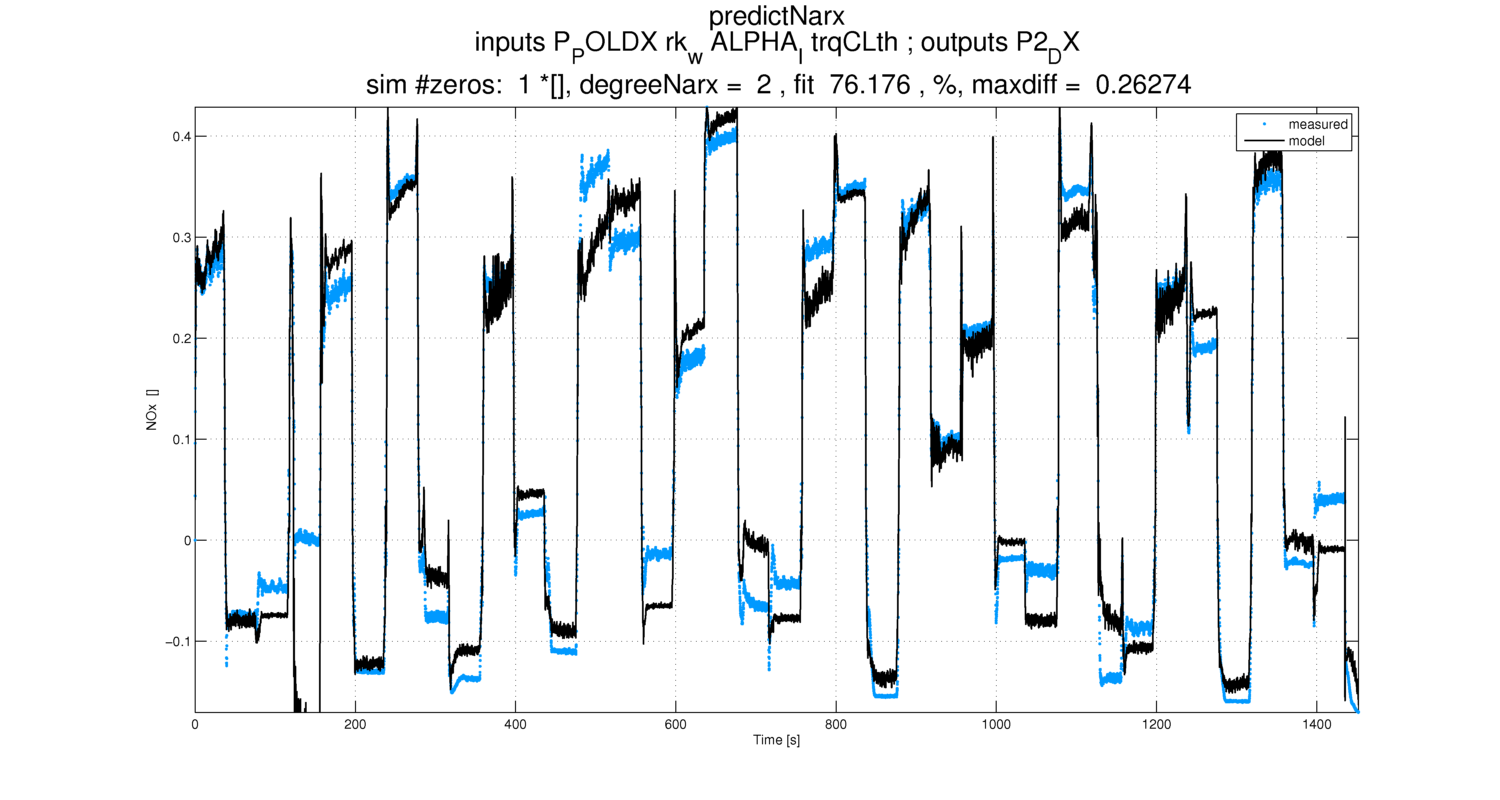
\includegraphics[width=.9\columnwidth]{Immagini/inputsP_POLDXrk_wALPHA_ItrqCLthoutputsP2_DX-predictNarx-3}
		\label{fig:inputsP_POLDXrk_wALPHA_ItrqCLthoutputsP2_DX-predictNarx-3}
	}
	\\
	\subfloat[P2 DX: Narx simulation]{
		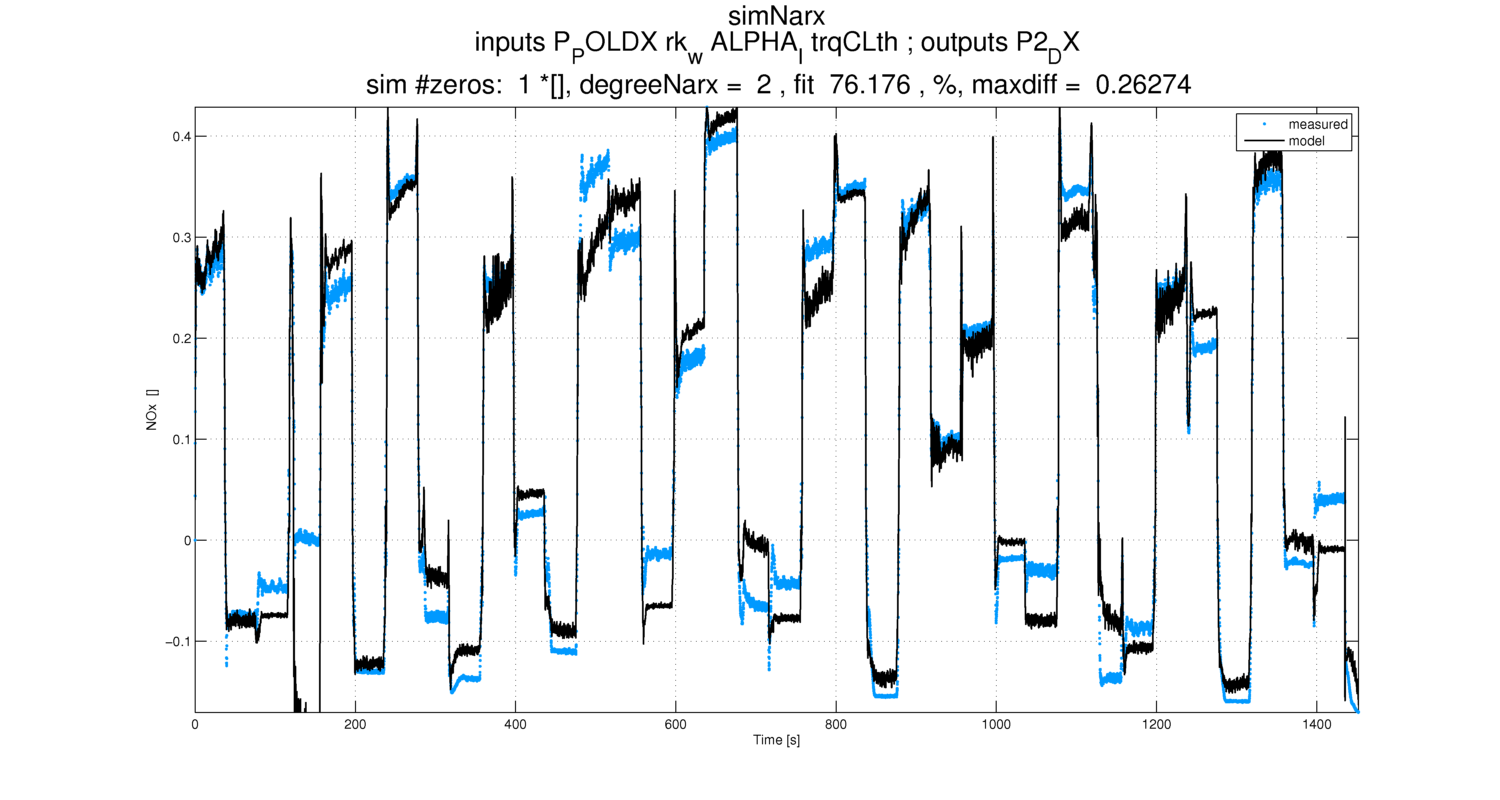
\includegraphics[width=.9\columnwidth]{Immagini/inputsP_POLDXrk_wALPHA_ItrqCLthoutputsP2_DX-simNarx-3}
		\label{fig:inputsP_POLDXrk_wALPHA_ItrqCLthoutputsP2_DX-simNarx-3}
	}
\phantomcaption
\end{figure}


\begin{figure}[htbp] \ContinuedFloat
	\centering 
	\subfloat[P2 DX: Transfer function identification]{
		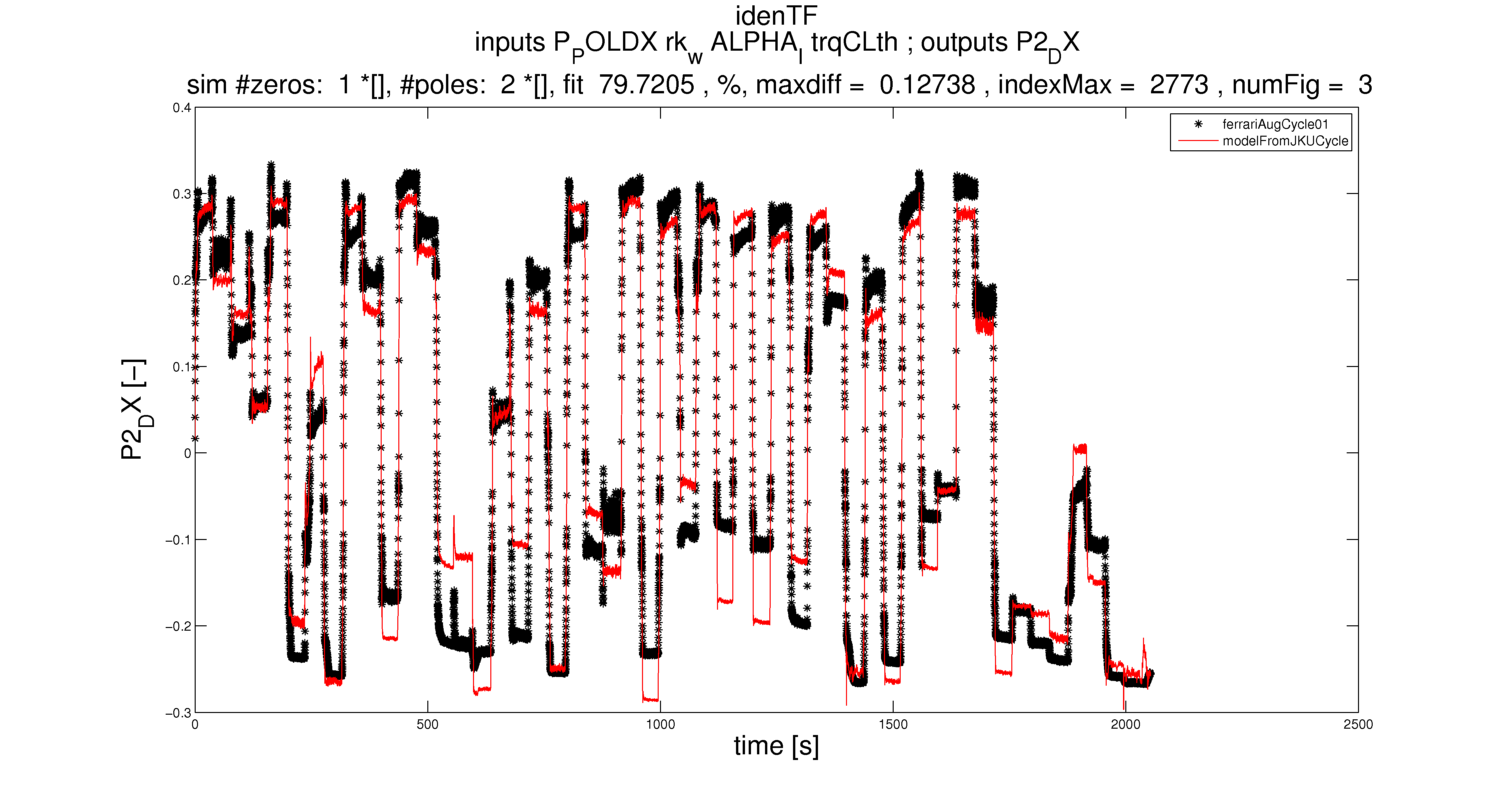
\includegraphics[width=.9\columnwidth]{Immagini/inputsP_POLDXrk_wALPHA_ItrqCLthoutputsP2_DX-idenTF-3}
		\label{fig:inputsP_POLDXrk_wALPHA_ItrqCLthoutputsP2_DX-idenTF-3}  }
	\\
	\subfloat[P2 DX: Transfer function simulation]{
		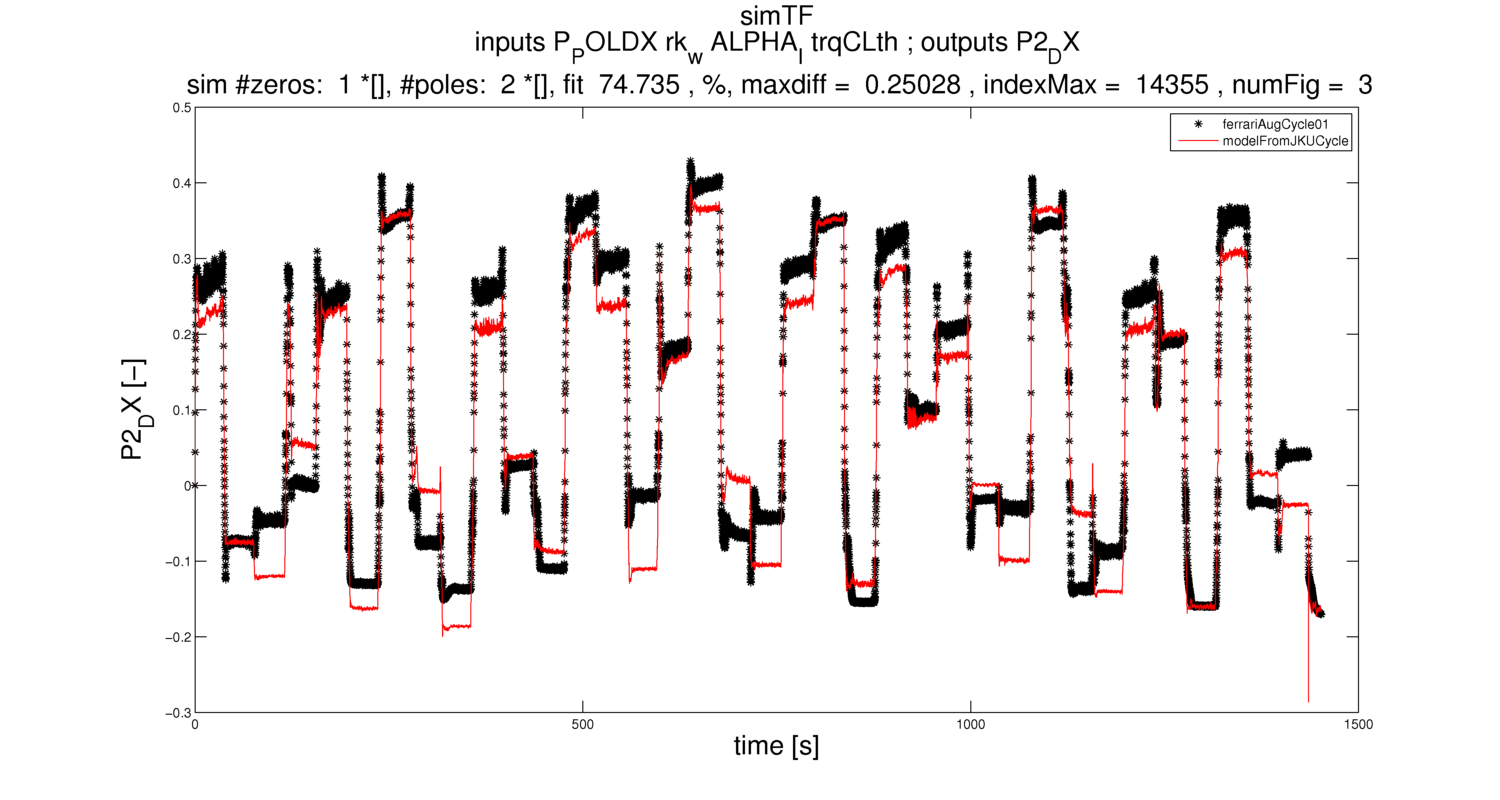
\includegraphics[width=.9\columnwidth]{Immagini/inputsP_POLDXrk_wALPHA_ItrqCLthoutputsP2_DX-simTF-3}
		\label{fig:inputsP_POLDXrk_wALPHA_ItrqCLthoutputsP2_DX-simTF-3}  }
	\\	
	\caption[Inputs: P POLDX, rk w, ALPHA I, trqCLth; Output: P2DX; np: 2; nz: 1; degree: 2]{Inputs: P POLDX, rk w, ALPHA I, trqCLth; Output: P2DX; np: 2; nz: 1; degree: 2}
	\label{fig:inputsP_POLDXrk_wALPHA_ItrqCLthoutputsP2_DX-3}
\end{figure}
%%inputsP_POLDXrk_wALPHA_ItrqCLthoutputsP2_DX-4.tex

\begin{figure}[htbp]
	\centering 
	\subfloat[P2 DX: Narx identification]{
		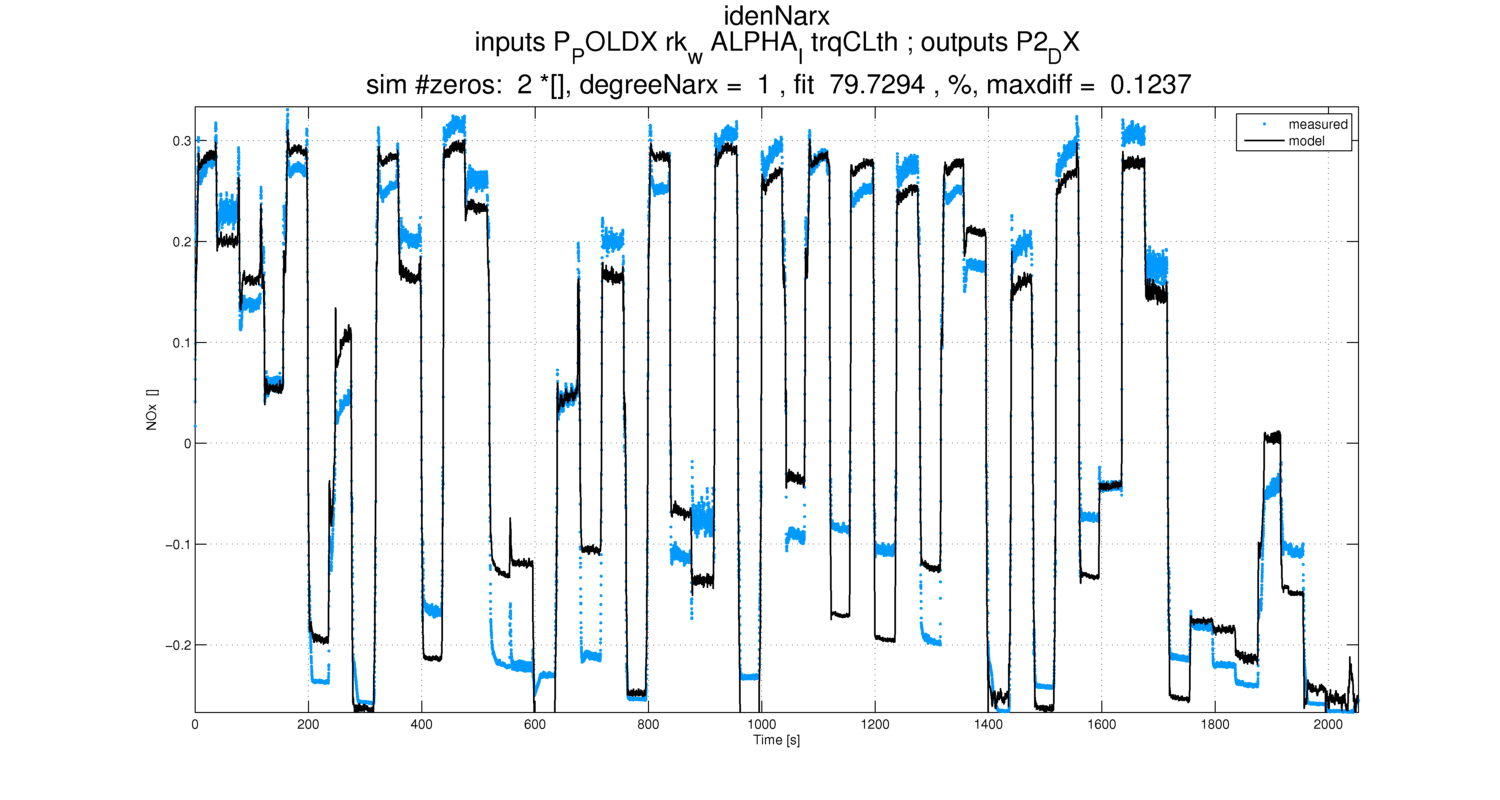
\includegraphics[width=.9\columnwidth]{Immagini/inputsP_POLDXrk_wALPHA_ItrqCLthoutputsP2_DX-idenNarx-4}
		\label{fig:inputsP_POLDXrk_wALPHA_ItrqCLthoutputsP2_DX-idenNarx-4}	}
	\\
	\subfloat[P2 DX: Narx prediction]{
		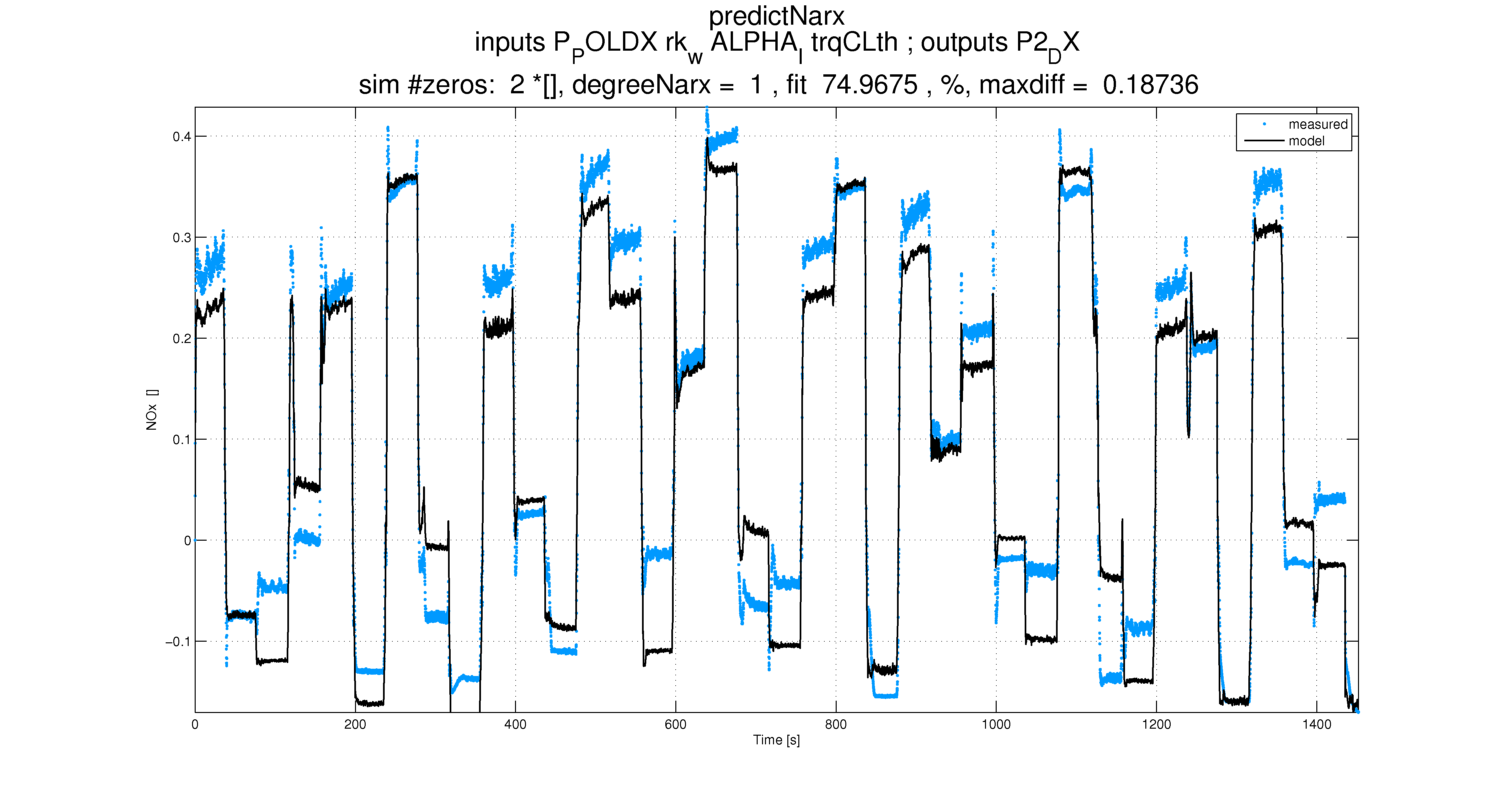
\includegraphics[width=.9\columnwidth]{Immagini/inputsP_POLDXrk_wALPHA_ItrqCLthoutputsP2_DX-predictNarx-4}
		\label{fig:inputsP_POLDXrk_wALPHA_ItrqCLthoutputsP2_DX-predictNarx-4}
	}
	\\
	\subfloat[P2 DX: Narx simulation]{
		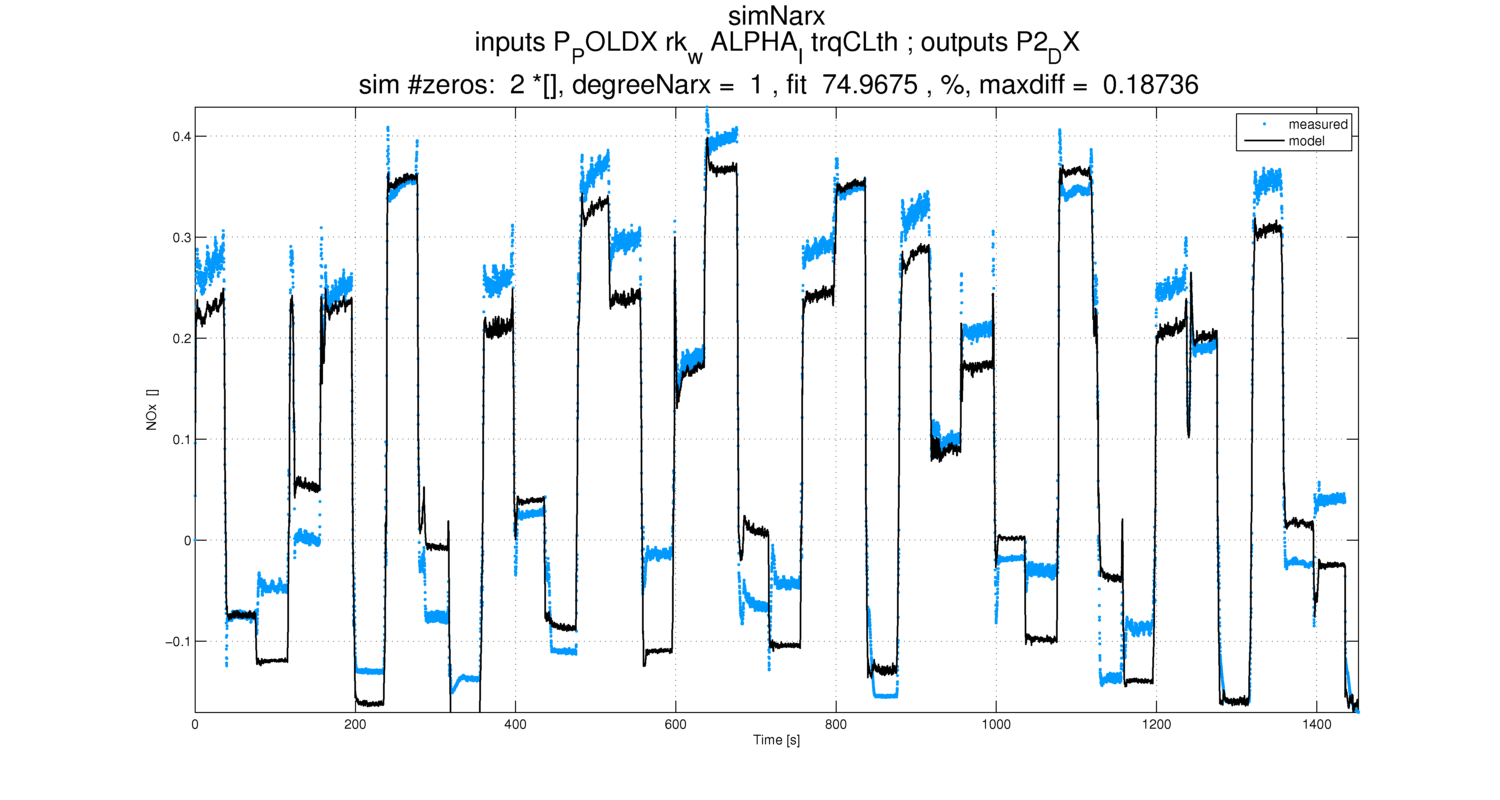
\includegraphics[width=.9\columnwidth]{Immagini/inputsP_POLDXrk_wALPHA_ItrqCLthoutputsP2_DX-simNarx-4}
		\label{fig:inputsP_POLDXrk_wALPHA_ItrqCLthoutputsP2_DX-simNarx-4}
	}
\phantomcaption
\end{figure}


\begin{figure}[htbp] \ContinuedFloat
	\centering 
	\subfloat[P2 DX: Transfer function identification]{
		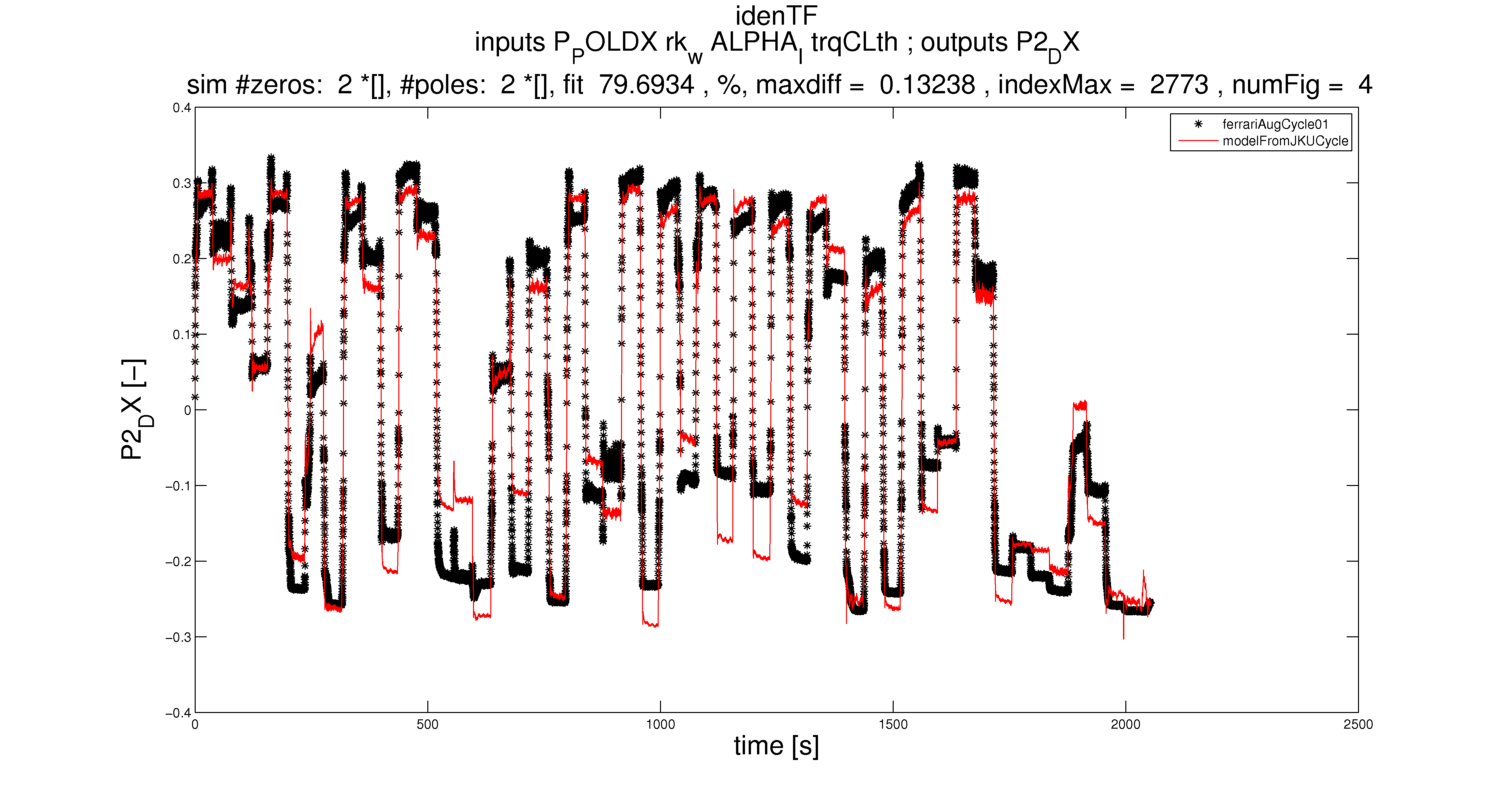
\includegraphics[width=.9\columnwidth]{Immagini/inputsP_POLDXrk_wALPHA_ItrqCLthoutputsP2_DX-idenTF-4}
		\label{fig:inputsP_POLDXrk_wALPHA_ItrqCLthoutputsP2_DX-idenTF-4}  }
	\\
	\subfloat[P2 DX: Transfer function simulation]{
		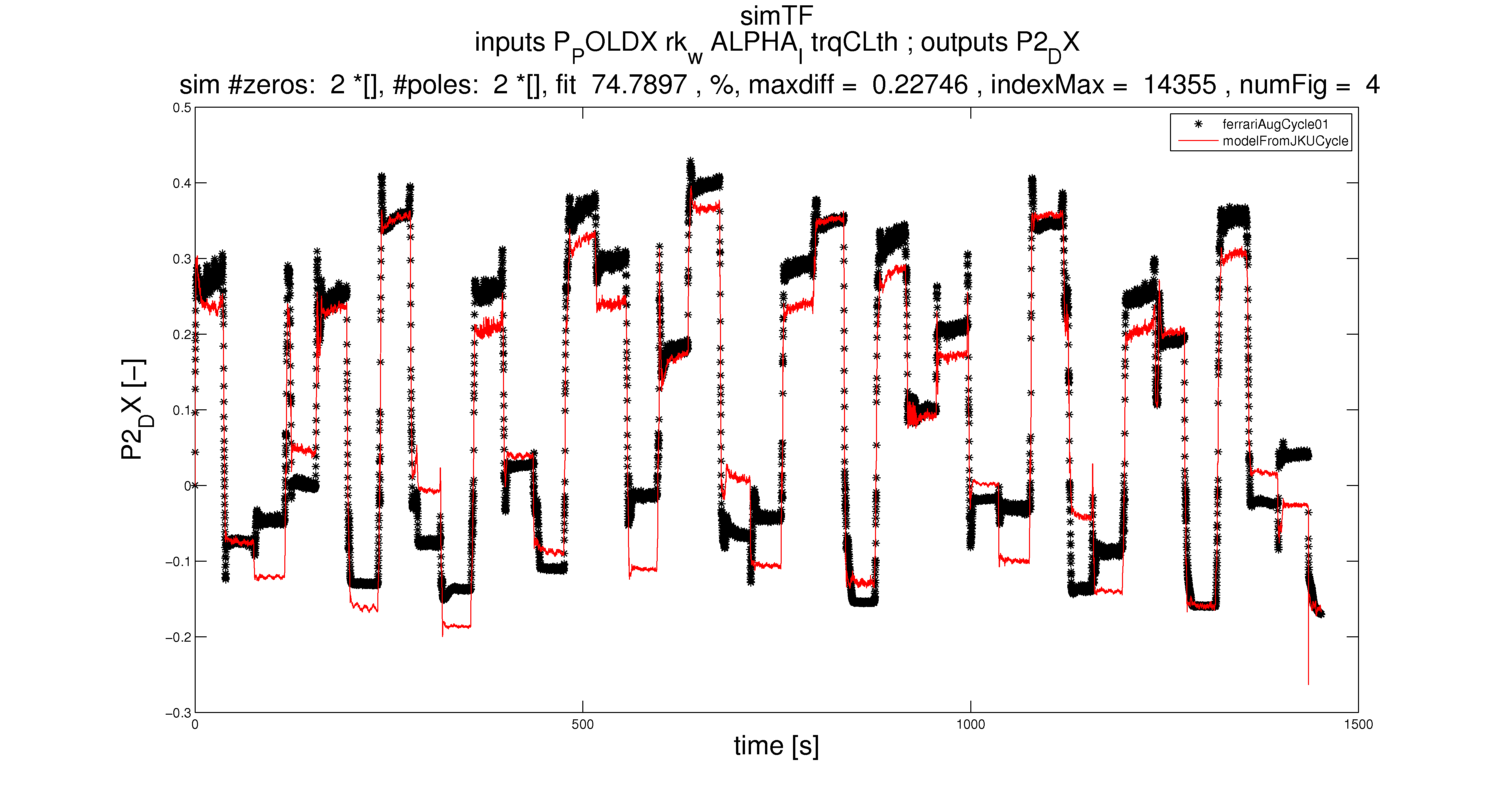
\includegraphics[width=.9\columnwidth]{Immagini/inputsP_POLDXrk_wALPHA_ItrqCLthoutputsP2_DX-simTF-4}
		\label{fig:inputsP_POLDXrk_wALPHA_ItrqCLthoutputsP2_DX-simTF-4}  }
	\\	
	\caption[Inputs: P POLDX, rk w, ALPHA I, trqCLth; Output: P2DX; np: 2; nz: 2; degree: 1]{Inputs: P POLDX, rk w, ALPHA I, trqCLth; Output: P2DX; np: 2; nz: 2; degree: 1}
	\label{fig:inputsP_POLDXrk_wALPHA_ItrqCLthoutputsP2_DX-4}
\end{figure}

\newpage

\subsection{Turbocharger right way out air temperature(T2 DX)}
\begin{itemize}
	\item{inputs:right turbo revolutions (giri tdx)}
	\item{output: turbocharger right way out air temperature(T2 DX)}
\end{itemize}

\begin{center} 
\begin{longtable}{ll|cccc|ccc|ccc} 
\caption[inputs GIRI TDX   outputs T2 DX]{inputs GIRI TDX   outputs T2 DX.} 
\label{tab:inputs_GIRI_TDX___outputs_T2_DX} 
\hline 
  mdl & type & np & nz & dPl & oY & ft100 & mxDf100 & mse100 & ft200 & mxDf200 & mse200 \\ 
 \hline 
tf  & iden & 1 & 1 & 0 & 0 & 59.6 & 0.29 & 0.00 & 59.3 & 0.29 & 0.00 \\ 
tf  & sim & 1 & 1 & 0 & 0 & 46.6 & 0.26 & 0.00 & 46.0 & 0.26 & 0.00 \\ 
 \hline 
tf  & iden & 1 & 2 & 0 & 0 & 59.9 & 0.29 & 0.00 & 60.1 & 0.28 & 0.00 \\ 
tf  & sim & 1 & 2 & 0 & 0 & 48.6 & 0.23 & 0.00 & 49.9 & 0.21 & 0.00 \\ 
 \hline 
tf  & iden & 2 & 1 & 0 & 0 & 59.7 & 0.29 & 0.00 & 59.6 & 0.29 & 0.00 \\ 
tf  & sim & 2 & 1 & 0 & 0 & 47.0 & 0.25 & 0.00 & 46.9 & 0.25 & 0.00 \\ 
 \hline 
tf  & iden & 2 & 2 & 0 & 0 & 62.0 & 0.24 & 0.00 & 61.9 & 0.23 & 0.00 \\ 
tf  & sim & 2 & 2 & 0 & 0 & 54.6 & 0.19 & 0.00 & 54.6 & 0.19 & 0.00 \\ 
 \hline 
\end{longtable} 
\end{center}

%%inputsGIRI_TDXoutputsT2_DX-1.tex

\begin{figure}[htbp]
	\centering 
	\subfloat[T2 DX: Narx identification]{
		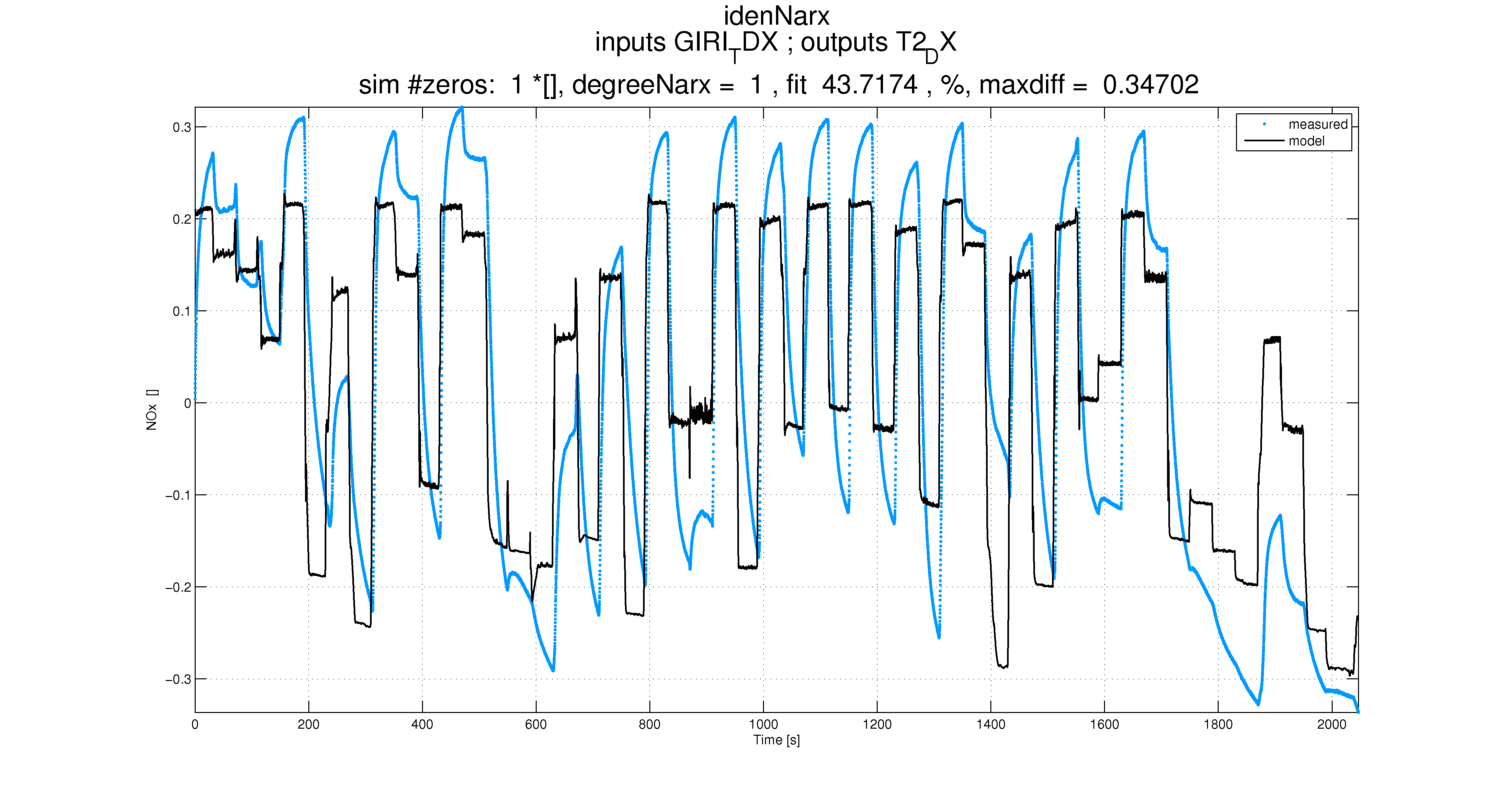
\includegraphics[width=.90\columnwidth]{Immagini/inputsGIRI_TDXoutputsT2_DX-idenNarx-1}
		\label{fig:inputsGIRI_TDXoutputsT2_DX-idenNarx-1}	}
	\\
	\subfloat[T2 DX: Narx prediction]{
		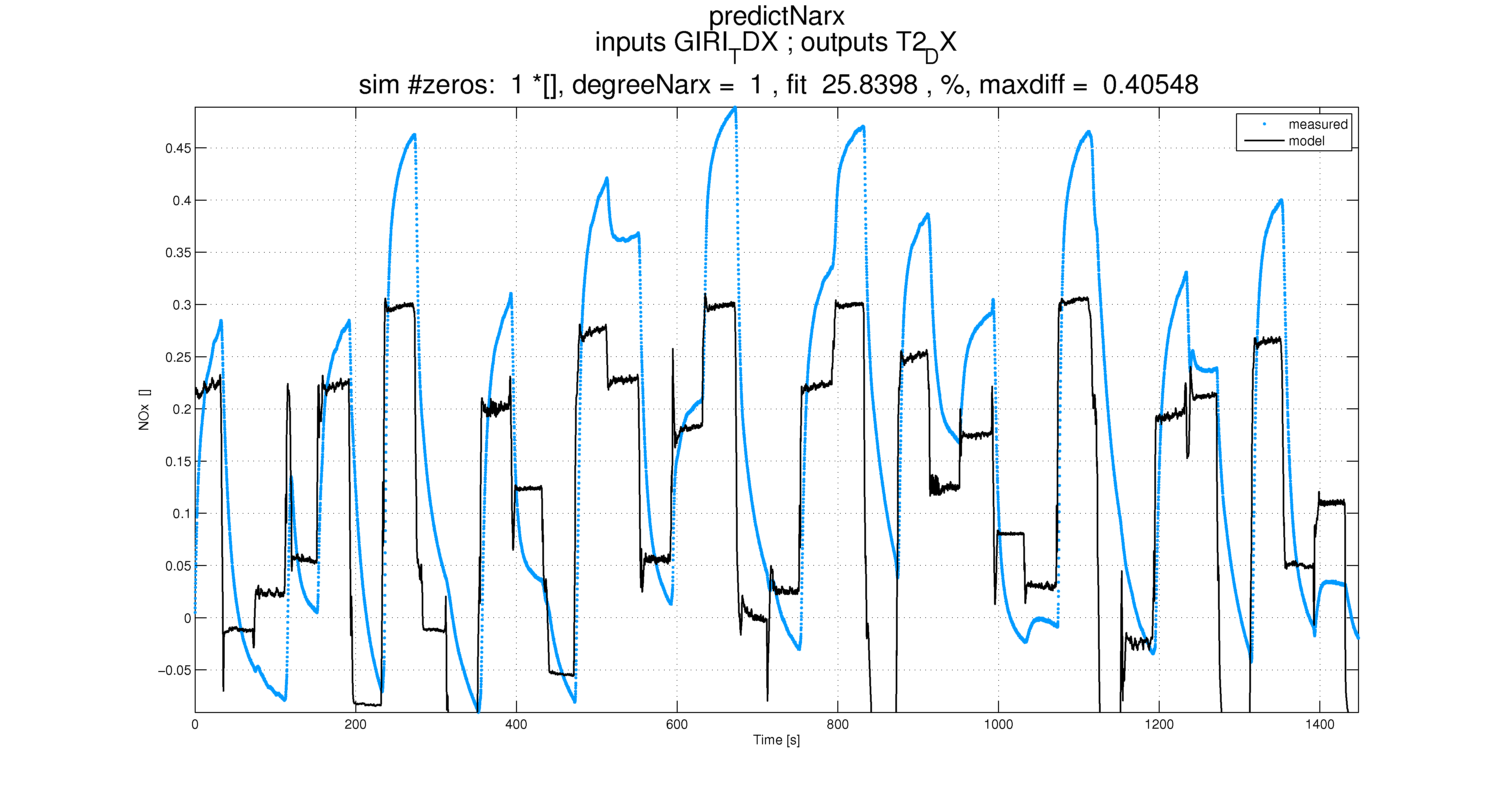
\includegraphics[width=.90\columnwidth]{Immagini/inputsGIRI_TDXoutputsT2_DX-predictNarx-1}
		\label{fig:inputsGIRI_TDXoutputsT2_DX-predictNarx-1}
	}
	\\
	\subfloat[T2 DX: Narx simulation]{
		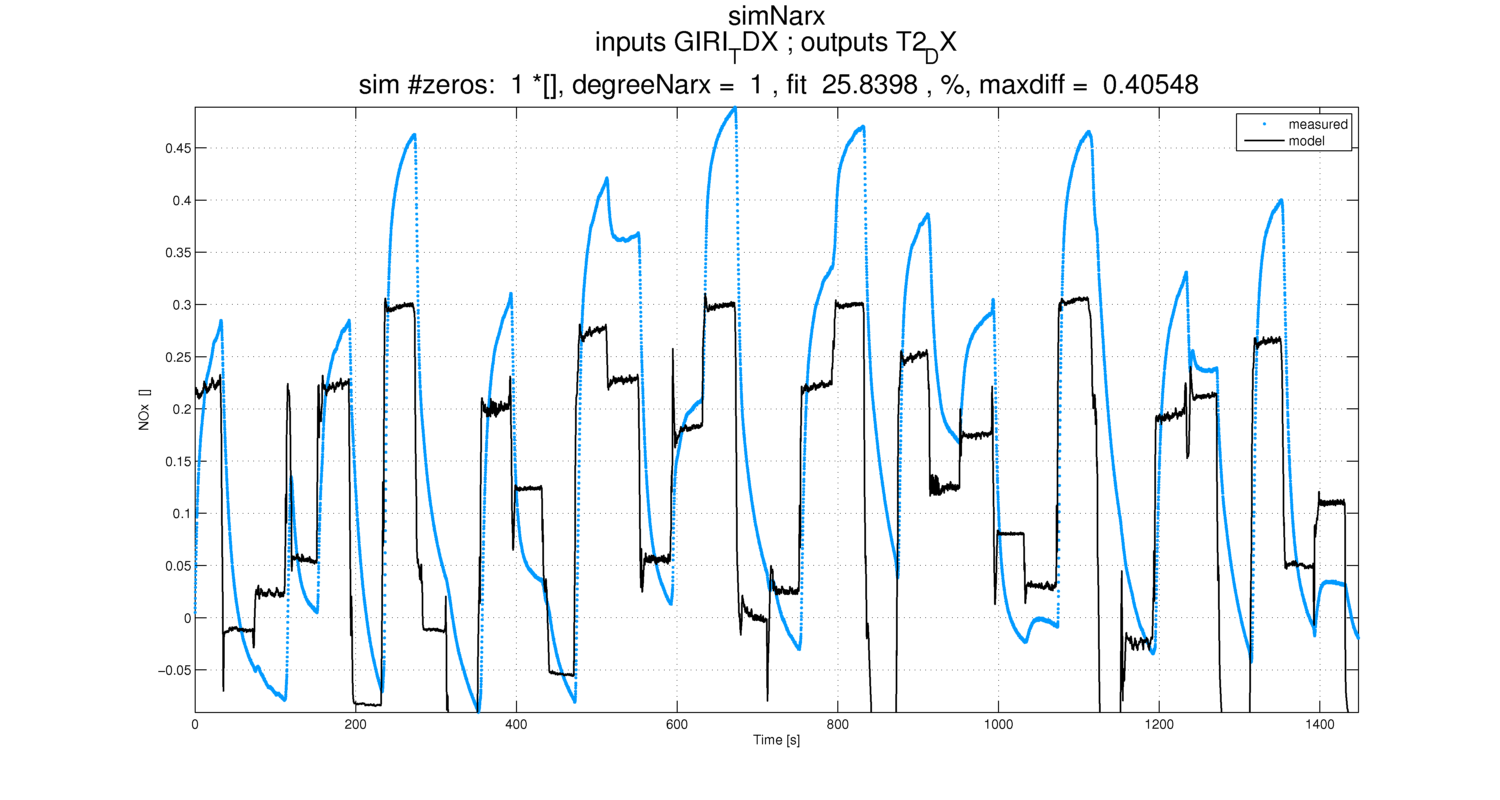
\includegraphics[width=.90\columnwidth]{Immagini/inputsGIRI_TDXoutputsT2_DX-simNarx-1}
		\label{fig:inputsGIRI_TDXoutputsT2_DX-simNarx-1}
	}
\phantomcaption
\end{figure}


\begin{figure}[htbp] \ContinuedFloat
	\centering 
	\subfloat[T2 DX: Transfer function identification]{
		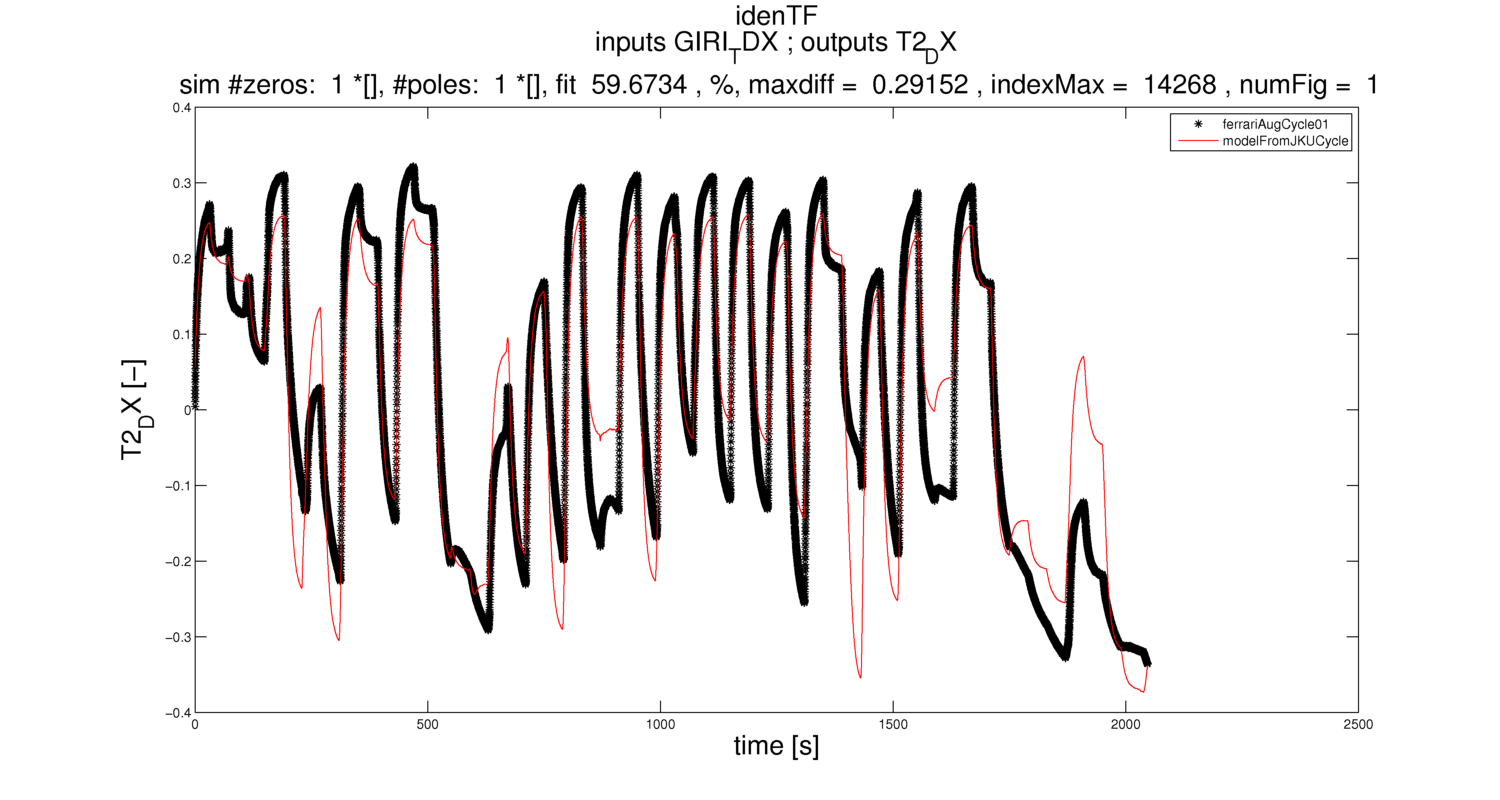
\includegraphics[width=.90\columnwidth]{Immagini/inputsGIRI_TDXoutputsT2_DX-idenTF-1}
		\label{fig:inputsGIRI_TDXoutputsT2_DX-idenTF-1}  }
	\\
	\subfloat[T2 DX: Transfer function simulation]{
		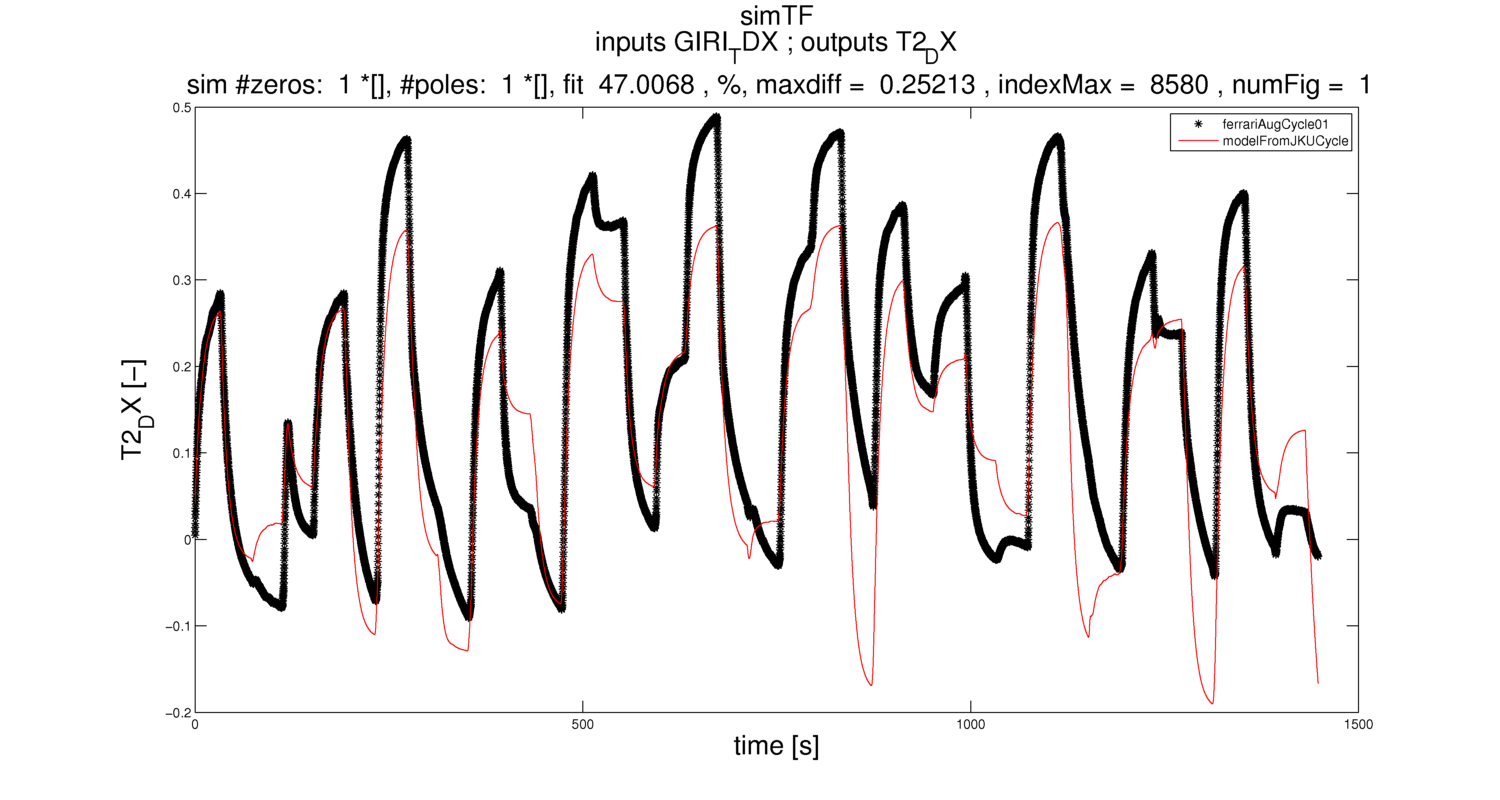
\includegraphics[width=.90\columnwidth]{Immagini/inputsGIRI_TDXoutputsT2_DX-simTF-1}
		\label{fig:inputsGIRI_TDXoutputsT2_DX-simTF-1}  }
	\\	
	\caption[Inputs: GIRI TDX; Output: T2DX; np: 1; nz: 1; degree: 1]{Inputs: GIRI TDX; Output: T2DX; np: 1; nz: 1; degree: 1}
	\label{fig:inputsGIRI_TDXoutputsT2_DX-1}
\end{figure}
%%inputsGIRI_TDXoutputsT2_DX-2.tex

\begin{figure}[htbp]
	\centering 
	\subfloat[T2 DX: Narx identification]{
		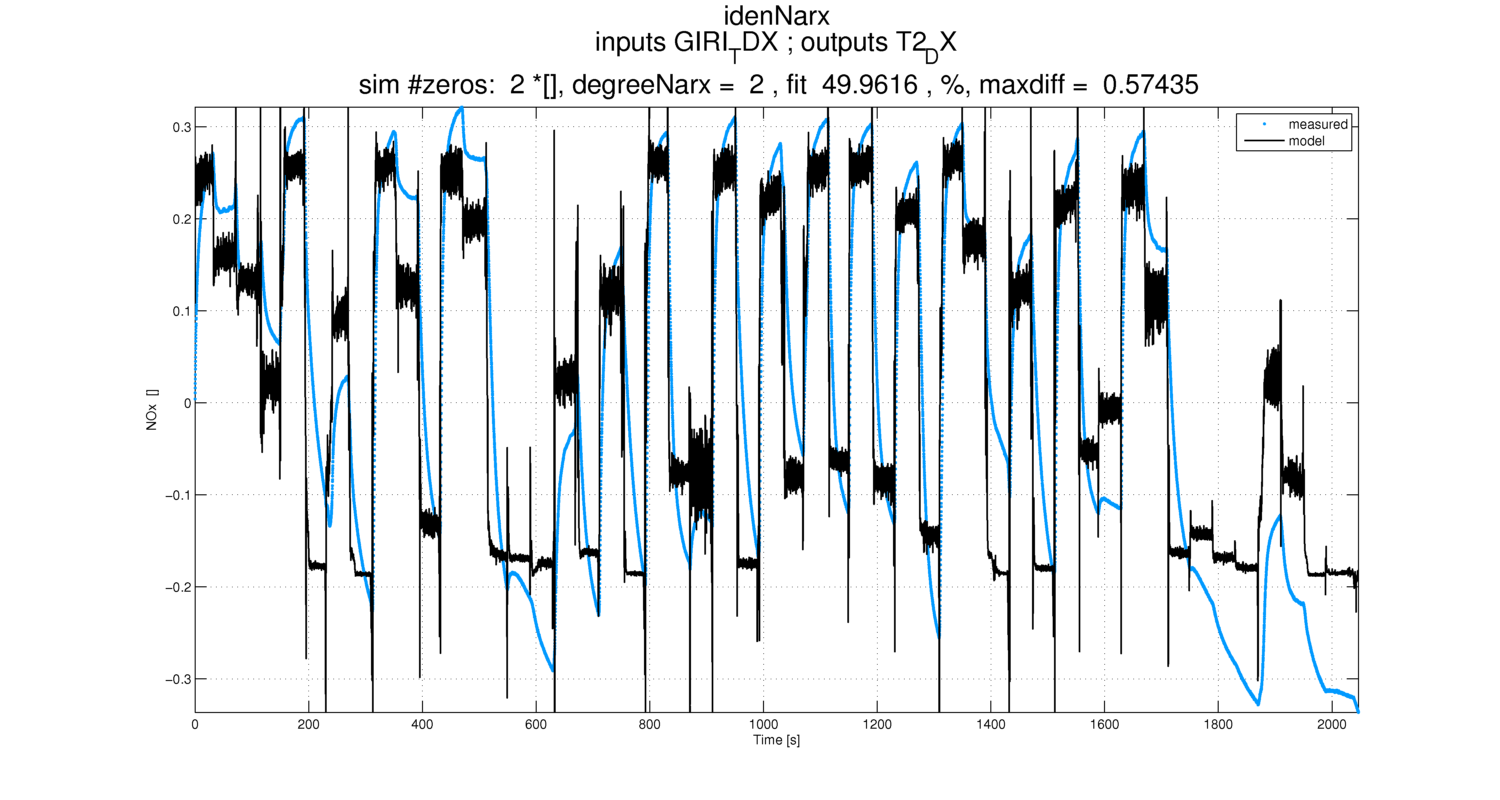
\includegraphics[width=.90\columnwidth]{Immagini/inputsGIRI_TDXoutputsT2_DX-idenNarx-2}
		\label{fig:inputsGIRI_TDXoutputsT2_DX-idenNarx-2}	}
	\\
	\subfloat[T2 DX: Narx prediction]{
		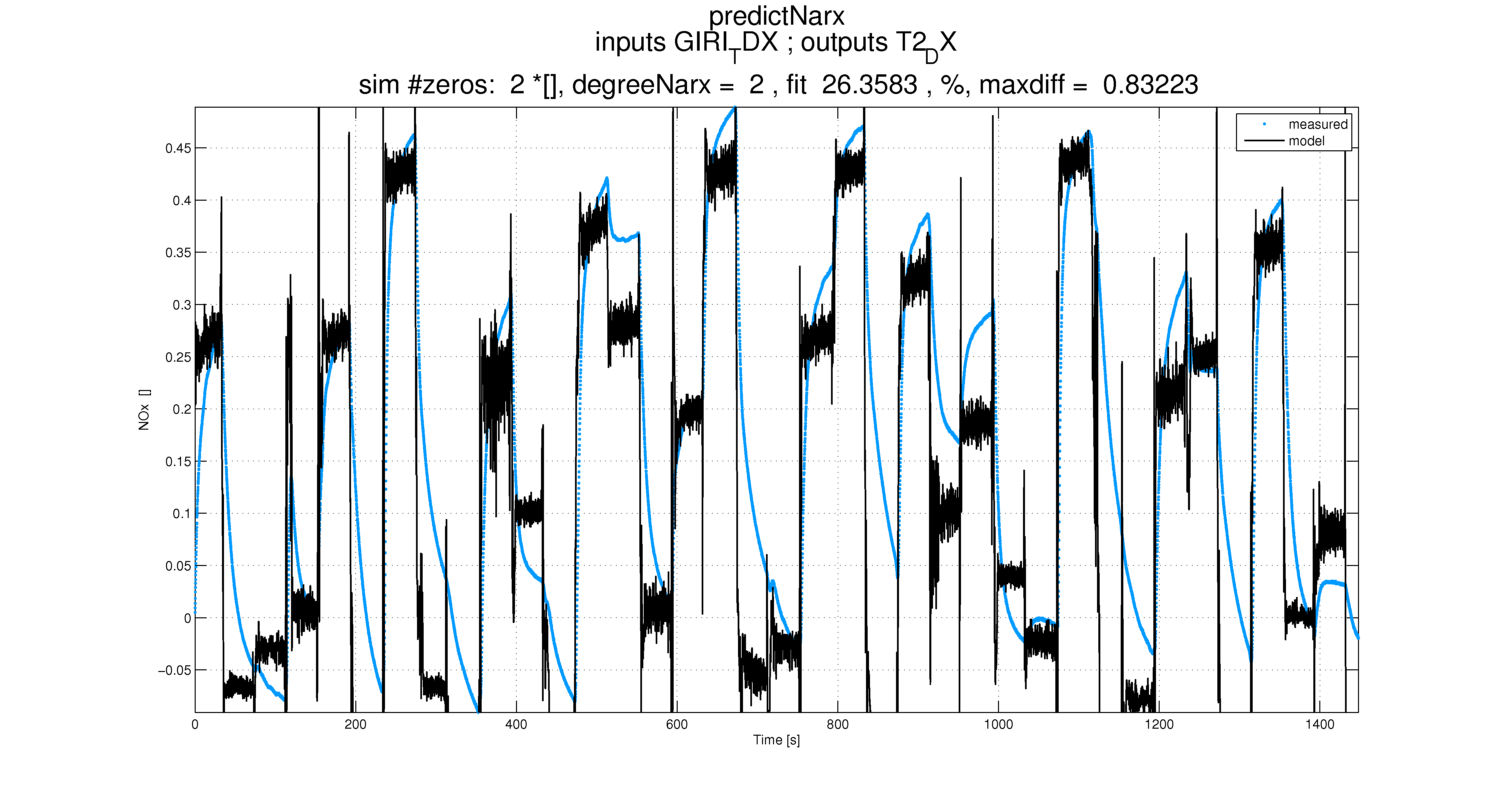
\includegraphics[width=.90\columnwidth]{Immagini/inputsGIRI_TDXoutputsT2_DX-predictNarx-2}
		\label{fig:inputsGIRI_TDXoutputsT2_DX-predictNarx-2}
	}
	\\
	\subfloat[T2 DX: Narx simulation]{
		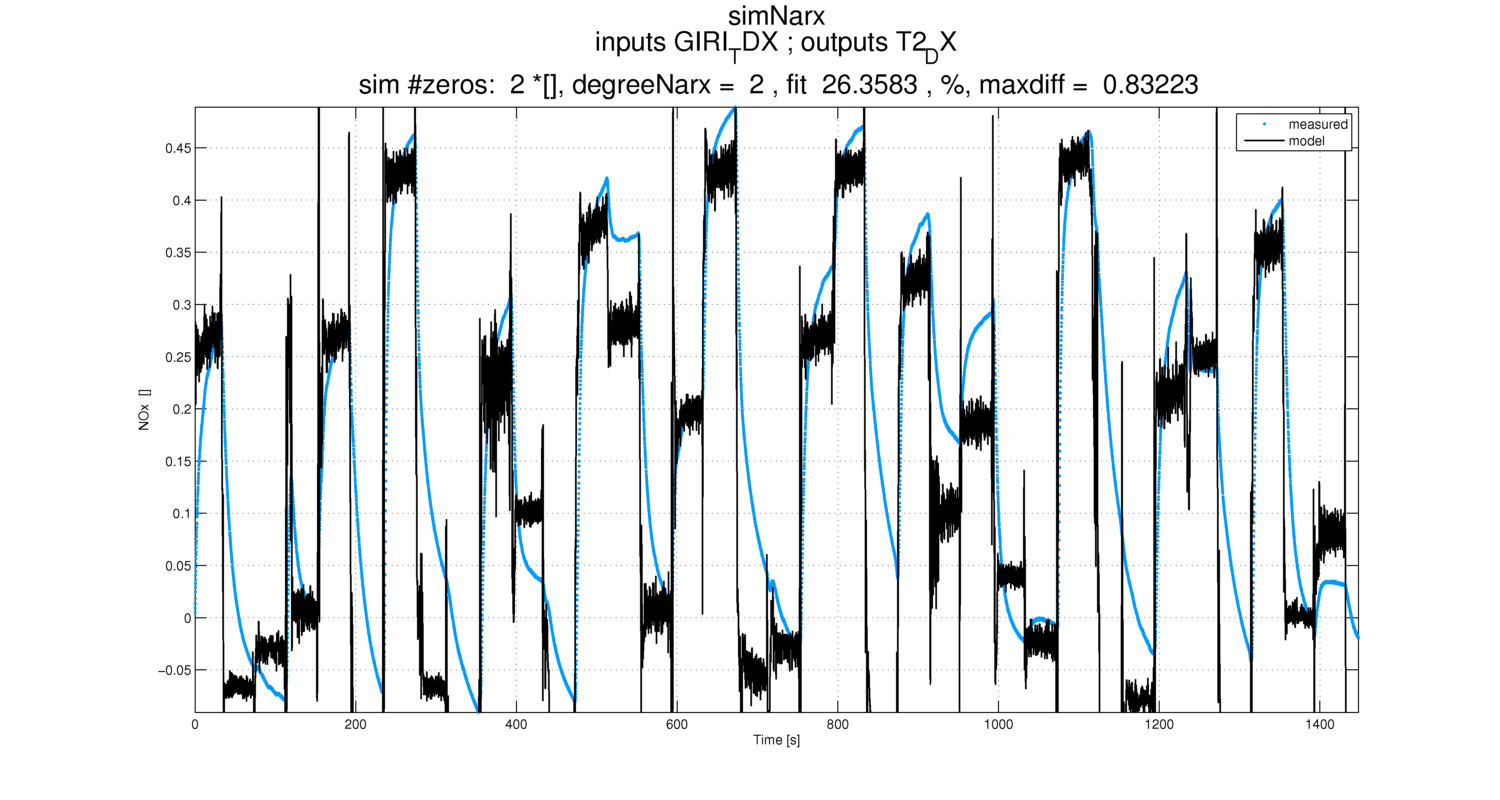
\includegraphics[width=.90\columnwidth]{Immagini/inputsGIRI_TDXoutputsT2_DX-simNarx-2}
		\label{fig:inputsGIRI_TDXoutputsT2_DX-simNarx-2}
	}
\phantomcaption
\end{figure}


\begin{figure}[htbp] \ContinuedFloat
	\centering 
	\subfloat[T2 DX: Transfer function identification]{
		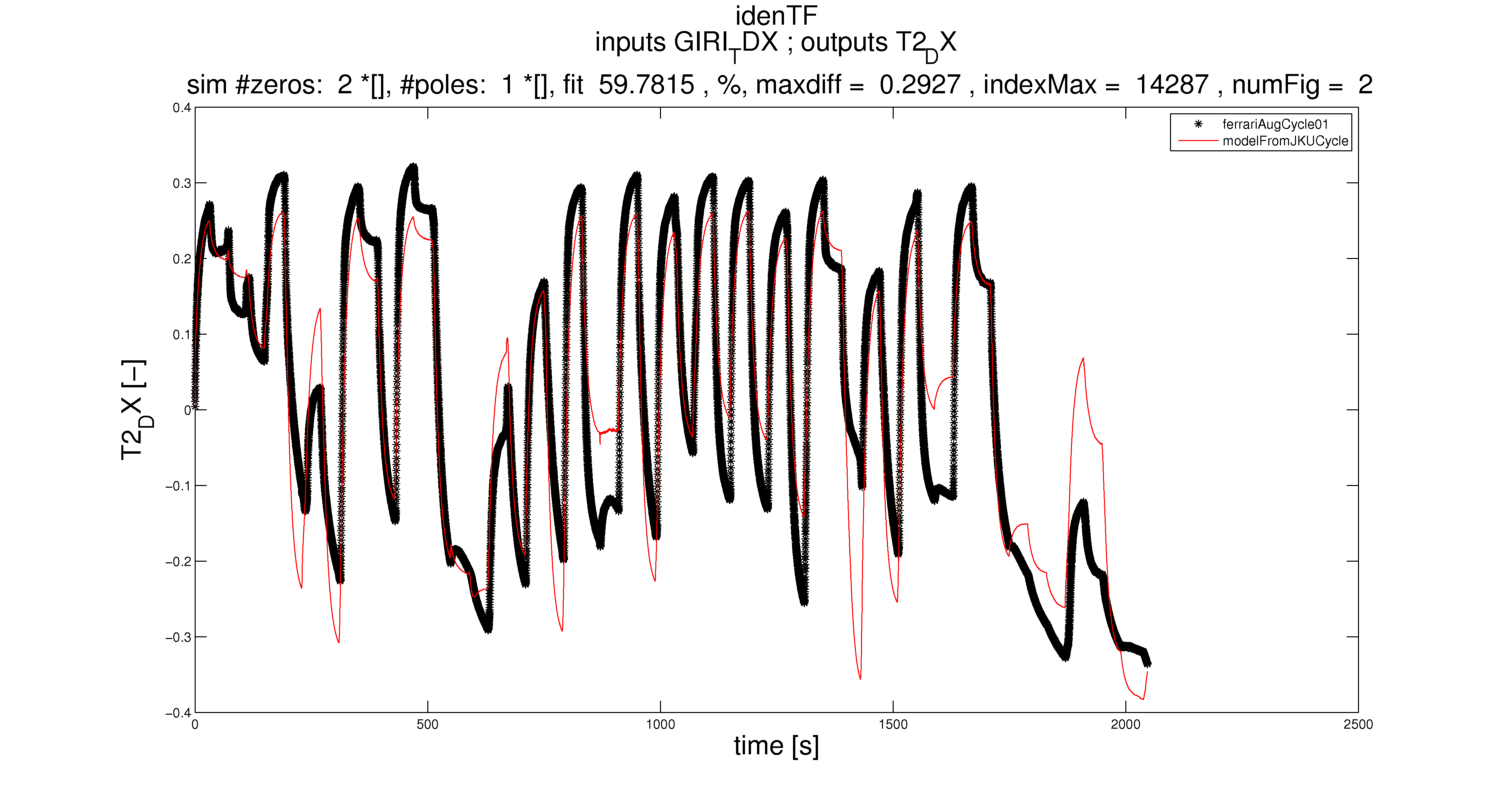
\includegraphics[width=.90\columnwidth]{Immagini/inputsGIRI_TDXoutputsT2_DX-idenTF-2}
		\label{fig:inputsGIRI_TDXoutputsT2_DX-idenTF-2}  }
	\\
	\subfloat[T2 DX: Transfer function simulation]{
		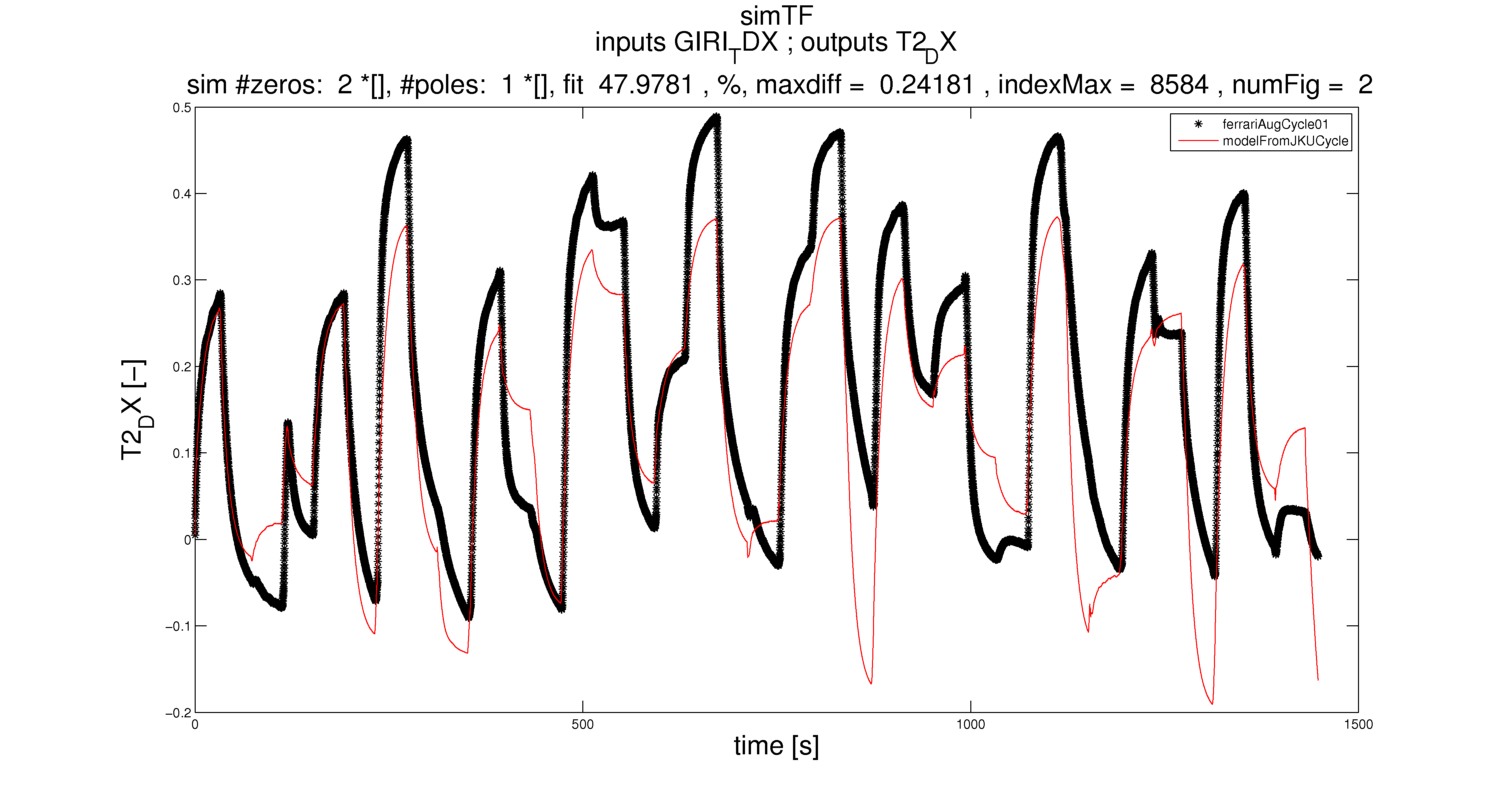
\includegraphics[width=.90\columnwidth]{Immagini/inputsGIRI_TDXoutputsT2_DX-simTF-2}
		\label{fig:inputsGIRI_TDXoutputsT2_DX-simTF-2}  }
	\\	
	\caption[Inputs: GIRI TDX; Output: T2DX; np: 1; nz: 2; degree: 2]{Inputs: GIRI TDX; Output: T2DX; np: 1; nz: 2; degree: 2}
	\label{fig:inputsGIRI_TDXoutputsT2_DX-2}
\end{figure}
%%inputsGIRI_TDXoutputsT2_DX-13.tex

\begin{figure}[htbp]
	\centering 
	\subfloat[T2 DX: Narx identification]{
		\includegraphics[width=.90\columnwidth]{Immagini/inputsGIRI_TDXoutputsT2_DX-idenNarx-3}
		\label{fig:inputsGIRI_TDXoutputsT2_DX-idenNarx-3}	}
	\\
	\subfloat[T2 DX: Narx prediction]{
		\includegraphics[width=.90\columnwidth]{Immagini/inputsGIRI_TDXoutputsT2_DX-predictNarx-3}
		\label{fig:inputsGIRI_TDXoutputsT2_DX-predictNarx-3}
	}
	\\
	\subfloat[T2 DX: Narx simulation]{
		\includegraphics[width=.90\columnwidth]{Immagini/inputsGIRI_TDXoutputsT2_DX-simNarx-3}
		\label{fig:inputsGIRI_TDXoutputsT2_DX-simNarx-3}
	}
\phantomcaption
\end{figure}


\begin{figure}[htbp] \ContinuedFloat
	\centering 
	\subfloat[T2 DX: Transfer function identification]{
		\includegraphics[width=.90\columnwidth]{Immagini/inputsGIRI_TDXoutputsT2_DX-idenTF-3}
		\label{fig:inputsGIRI_TDXoutputsT2_DX-idenTF-3}  }
	\\
	\subfloat[T2 DX: Transfer function simulation]{
		\includegraphics[width=.90\columnwidth]{Immagini/inputsGIRI_TDXoutputsT2_DX-simTF-3}
		\label{fig:inputsGIRI_TDXoutputsT2_DX-simTF-3}  }
	\\	
	\caption[Inputs: GIRI TDX; Output: T2DX; np: 2; nz: 1; degree: 2]{Inputs: GIRI TDX; Output: T2DX; np: 2; nz: 1; degree: 2}
	\label{fig:inputsGIRI_TDXoutputsT2_DX-1}
\end{figure}
%%inputsGIRI_TDXoutputsT2_DX-4.tex

\begin{figure}[htbp]
	\centering 
	\subfloat[T2 DX: Narx identification]{
		\includegraphics[width=.90\columnwidth]{Immagini/inputsGIRI_TDXoutputsT2_DX-idenNarx-4}
		\label{fig:inputsGIRI_TDXoutputsT2_DX-idenNarx-4}	}
	\\
	\subfloat[T2 DX: Narx prediction]{
		\includegraphics[width=.90\columnwidth]{Immagini/inputsGIRI_TDXoutputsT2_DX-predictNarx-4}
		\label{fig:inputsGIRI_TDXoutputsT2_DX-predictNarx-4}
	}
	\\
	\subfloat[T2 DX: Narx simulation]{
		\includegraphics[width=.90\columnwidth]{Immagini/inputsGIRI_TDXoutputsT2_DX-simNarx-4}
		\label{fig:inputsGIRI_TDXoutputsT2_DX-simNarx-4}
	}
\phantomcaption
\end{figure}


\begin{figure}[htbp] \ContinuedFloat
	\centering 
	\subfloat[T2 DX: Transfer function identification]{
		\includegraphics[width=.90\columnwidth]{Immagini/inputsGIRI_TDXoutputsT2_DX-idenTF-4}
		\label{fig:inputsGIRI_TDXoutputsT2_DX-idenTF-4}  }
	\\
	\subfloat[T2 DX: Transfer function simulation]{
		\includegraphics[width=.90\columnwidth]{Immagini/inputsGIRI_TDXoutputsT2_DX-simTF-4}
		\label{fig:inputsGIRI_TDXoutputsT2_DX-simTF-4}  }
	\\	
	\caption[Inputs: GIRI TDX; Output: T2DX; np: 2; nz: 2; degree: 1]{Inputs: GIRI TDX; Output: T2DX; np: 2; nz: 2; degree: 1}
	\label{fig:inputsGIRI_TDXoutputsT2_DX-4}
\end{figure}

\newpage

\subsection{Intercooler right way out air pressure(P5 DX)}
\begin{itemize}
	\item{inputs: turbocharger right way out air pressure (p2 dx), boost pressure (pvd w)}
	\item{output: Intercooler right way out air pressure(P5 DX)}
\end{itemize}

\begin{center} 
\begin{longtable}{ll|cccc|ccc|ccc} 
\caption[inputs P2 DX pvd w   outputs P5 DX]{inputs P2 DX pvd w   outputs P5 DX.} 
\label{tab:inputs_P2_DX_pvd_w___outputs_P5_DX} 
\hline 
  mdl & type & np & nz & dPl & oY & ft100 & mxDf100 & mse100 & ft200 & mxDf200 & mse200 \\ 
 \hline 
tf  & iden & 1 & 1 & 0 & 0 & 86.4 & 0.28 & 0.00 & 76.4 & 0.42 & 0.00 \\ 
tf  & sim & 1 & 1 & 0 & 0 & 83.0 & 0.37 & 0.00 & 73.2 & 0.33 & 0.00 \\ 
 \hline 
tf  & iden & 1 & 2 & 0 & 0 & 87.4 & 0.26 & 0.00 & 77.4 & 0.38 & 0.00 \\ 
tf  & sim & 1 & 2 & 0 & 0 & 83.8 & 0.33 & 0.00 & 74.6 & 0.33 & 0.00 \\ 
 \hline 
tf  & iden & 2 & 1 & 0 & 0 & 86.9 & 0.28 & 0.00 & 76.7 & 0.41 & 0.00 \\ 
tf  & sim & 2 & 1 & 0 & 0 & 83.2 & 0.38 & 0.00 & 73.4 & 0.33 & 0.00 \\ 
 \hline 
tf  & iden & 2 & 2 & 0 & 0 & 87.5 & 0.26 & 0.00 & 77.0 & 0.40 & 0.00 \\ 
tf  & sim & 2 & 2 & 0 & 0 & 83.8 & 0.34 & 0.00 & 74.2 & 0.34 & 0.00 \\ 
 \hline 
\end{longtable} 
\end{center}

%%inputsP2_DXpvd_woutputsP5_DX-1.tex

\begin{figure}[htbp]
	\centering 
	\subfloat[T2 DX: Narx identification]{
		\includegraphics[width=.90\columnwidth]{Immagini/inputsP2_DXpvd_woutputsP5_DX-idenNarx-1}
		\label{fig:inputsP2_DXpvd_woutputsP5_DX-idenNarx-1}	}
	\\
	\subfloat[T2 DX: Narx prediction]{
		\includegraphics[width=.90\columnwidth]{Immagini/inputsP2_DXpvd_woutputsP5_DX-predictNarx-1}
		\label{fig:inputsP2_DXpvd_woutputsP5_DX-predictNarx-1}
	}
	\\
	\subfloat[T2 DX: Narx simulation]{
		\includegraphics[width=.90\columnwidth]{Immagini/inputsP2_DXpvd_woutputsP5_DX-simNarx-1}
		\label{fig:inputsP2_DXpvd_woutputsP5_DX-simNarx-1}
	}
\phantomcaption
\end{figure}


\begin{figure}[htbp] \ContinuedFloat
	\centering 
	\subfloat[T2 DX: Transfer function identification]{
		\includegraphics[width=.90\columnwidth]{Immagini/inputsP2_DXpvd_woutputsP5_DX-idenTF-1}
		\label{fig:inputsP2_DXpvd_woutputsP5_DX-idenTF-1}  }
	\\
	\subfloat[T2 DX: Transfer function simulation]{
		\includegraphics[width=.90\columnwidth]{Immagini/inputsP2_DXpvd_woutputsP5_DX-simTF-1}
		\label{fig:inputsP2_DXpvd_woutputsP5_DX-simTF-1}  }
	\\	
	\caption[Inputs: P2 DX, pvd w; Output: P5 DX; np: 1; nz: 1; degree: 1]{Inputs: P2 DX, pvd w; Output: P5 DX; np: 1; nz: 1; degree: 1.}
	\label{fig:inputsP2_DXpvd_woutputsP5_DX-1}
\end{figure}
%%inputsP2_DXpvd_woutputsP5_DX-2.tex

\begin{figure}[htbp]
	\centering 
	\subfloat[T2 DX: Narx identification]{
		\includegraphics[width=.90\columnwidth]{Immagini/inputsP2_DXpvd_woutputsP5_DX-idenNarx-2}
		\label{fig:inputsP2_DXpvd_woutputsP5_DX-idenNarx-2}	}
	\\
	\subfloat[T2 DX: Narx prediction]{
		\includegraphics[width=.90\columnwidth]{Immagini/inputsP2_DXpvd_woutputsP5_DX-predictNarx-2}
		\label{fig:inputsP2_DXpvd_woutputsP5_DX-predictNarx-2}
	}
	\\
	\subfloat[T2 DX: Narx simulation]{
		\includegraphics[width=.90\columnwidth]{Immagini/inputsP2_DXpvd_woutputsP5_DX-simNarx-2}
		\label{fig:inputsP2_DXpvd_woutputsP5_DX-simNarx-2}
	}
\phantomcaption
\end{figure}


\begin{figure}[htbp] \ContinuedFloat
	\centering 
	\subfloat[T2 DX: Transfer function identification]{
		\includegraphics[width=.90\columnwidth]{Immagini/inputsP2_DXpvd_woutputsP5_DX-idenTF-2}
		\label{fig:inputsP2_DXpvd_woutputsP5_DX-idenTF-2}  }
	\\
	\subfloat[T2 DX: Transfer function simulation]{
		\includegraphics[width=.90\columnwidth]{Immagini/inputsP2_DXpvd_woutputsP5_DX-simTF-2}
		\label{fig:inputsP2_DXpvd_woutputsP5_DX-simTF-2}  }
	\\	
	\caption[Inputs: P2 DX, pvd w; Output: P5 DX; np: 1; nz: 2; degree: 2]{Inputs: P2 DX, pvd w; Output: P5 DX; np: 1; nz: 2; degree: 2.}
	\label{fig:inputsP2_DXpvd_woutputsP5_DX-2}
\end{figure}
%%inputsP2_DXpvd_woutputsP5_DX-3.tex

\begin{figure}[htbp]
	\centering 
	\subfloat[T2 DX: Narx identification]{
		\includegraphics[width=.90\columnwidth]{Immagini/inputsP2_DXpvd_woutputsP5_DX-idenNarx-3}
		\label{fig:inputsP2_DXpvd_woutputsP5_DX-idenNarx-3}	}
	\\
	\subfloat[T2 DX: Narx prediction]{
		\includegraphics[width=.90\columnwidth]{Immagini/inputsP2_DXpvd_woutputsP5_DX-predictNarx-3}
		\label{fig:inputsP2_DXpvd_woutputsP5_DX-predictNarx-3}
	}
	\\
	\subfloat[T2 DX: Narx simulation]{
		\includegraphics[width=.90\columnwidth]{Immagini/inputsP2_DXpvd_woutputsP5_DX-simNarx-3}
		\label{fig:inputsP2_DXpvd_woutputsP5_DX-simNarx-3}
	}
\phantomcaption
\end{figure}


\begin{figure}[htbp] \ContinuedFloat
	\centering 
	\subfloat[T2 DX: Transfer function identification]{
		\includegraphics[width=.90\columnwidth]{Immagini/inputsP2_DXpvd_woutputsP5_DX-idenTF-3}
		\label{fig:inputsP2_DXpvd_woutputsP5_DX-idenTF-3}  }
	\\
	\subfloat[T2 DX: Transfer function simulation]{
		\includegraphics[width=.90\columnwidth]{Immagini/inputsP2_DXpvd_woutputsP5_DX-simTF-3}
		\label{fig:inputsP2_DXpvd_woutputsP5_DX-simTF-3}  }
	\\	
	\caption[Inputs: P2 DX, pvd w; Output: P5 DX; np: 2; nz: 1; degree: 2]{Inputs: P2 DX, pvd w; Output: P5 DX; np: 2; nz: 1; degree: 2.}
	\label{fig:inputsP2_DXpvd_woutputsP5_DX-3}
\end{figure}
%%inputsP2_DXpvd_woutputsP5_DX-4.tex

\begin{figure}[htbp]
	\centering 
	\subfloat[T2 DX: Narx identification]{
		\includegraphics[width=.90\columnwidth]{Immagini/inputsP2_DXpvd_woutputsP5_DX-idenNarx-4}
		\label{fig:inputsP2_DXpvd_woutputsP5_DX-idenNarx-4}	}
	\\
	\subfloat[T2 DX: Narx prediction]{
		\includegraphics[width=.90\columnwidth]{Immagini/inputsP2_DXpvd_woutputsP5_DX-predictNarx-4}
		\label{fig:inputsP2_DXpvd_woutputsP5_DX-predictNarx-4}
	}
	\\
	\subfloat[T2 DX: Narx simulation]{
		\includegraphics[width=.90\columnwidth]{Immagini/inputsP2_DXpvd_woutputsP5_DX-simNarx-4}
		\label{fig:inputsP2_DXpvd_woutputsP5_DX-simNarx-4}
	}
\phantomcaption
\end{figure}


\begin{figure}[htbp] \ContinuedFloat
	\centering 
	\subfloat[T2 DX: Transfer function identification]{
		\includegraphics[width=.90\columnwidth]{Immagini/inputsP2_DXpvd_woutputsP5_DX-idenTF-4}
		\label{fig:inputsP2_DXpvd_woutputsP5_DX-idenTF-4}  }
	\\
	\subfloat[T2 DX: Transfer function simulation]{
		\includegraphics[width=.90\columnwidth]{Immagini/inputsP2_DXpvd_woutputsP5_DX-simTF-4}
		\label{fig:inputsP2_DXpvd_woutputsP5_DX-simTF-4}  }
	\\	
	\caption[Inputs: P2 DX, pvd w; Output: P5 DX; np: 2; nz: 2; degree: 1]{Inputs: P2 DX, pvd w; Output: P5 DX; np: 2; nz: 2; degree: 1.}
	\label{fig:inputsP2_DXpvd_woutputsP5_DX-4}
\end{figure}

\newpage

\subsection{Right turbo revolutions (giri tdx)} %37
\begin{itemize}
	\item{inputs:Right intake hydraulic tappets oil pressure (P PADX), Catalyst in pressure right side (P ICDX), Intercooler right way out air pressure(P5 DX)}
	\item{output: right turbo revolutions (giri tdx)}
\end{itemize}

\begin{center} 
\begin{longtable}{ll|cccc|ccc|ccc} 
\caption[inputs P PADX P ICDX P5 DX   outputs GIRI TDX]{inputs P PADX P ICDX P5 DX   outputs GIRI TDX.} 
\label{tab:inputs_P_PADX_P_ICDX_P5_DX___outputs_GIRI_TDX} 
\hline 
  mdl & type & np & nz & dPl & oY & ft100 & mxDf100 & mse100 & ft200 & mxDf200 & mse200 \\ 
 \hline 
tf  & iden & 1 & 1 & 0 & 0 & 78.7 & 0.33 & 0.00 & 73.3 & 0.50 & 0.00 \\ 
tf  & sim & 1 & 1 & 0 & 0 & 70.8 & 0.43 & 0.00 & 64.5 & 0.48 & 0.00 \\ 
 \hline 
tf  & iden & 1 & 2 & 0 & 0 & 78.8 & 0.32 & 0.00 & 73.4 & 0.50 & 0.00 \\ 
tf  & sim & 1 & 2 & 0 & 0 & 70.8 & 0.42 & 0.00 & 64.5 & 0.47 & 0.00 \\ 
 \hline 
tf  & iden & 2 & 1 & 0 & 0 & 74.3 & 0.42 & 0.00 & 70.3 & 0.52 & 0.00 \\ 
tf  & sim & 2 & 1 & 0 & 0 & 66.6 & 0.62 & 0.00 & 60.6 & 0.46 & 0.00 \\ 
 \hline 
tf  & iden & 2 & 2 & 0 & 0 & 79.3 & 0.33 & 0.00 & 73.8 & 0.49 & 0.00 \\ 
tf  & sim & 2 & 2 & 0 & 0 & 75.0 & 0.40 & 0.00 & 68.0 & 0.43 & 0.00 \\ 
 \hline 
narx & iden & 0 & 1 & 1 & 1 & 0.0 & 0.00 & 0.00 & 86.5 & 0.24 & 0.00 \\ 
narx & pred & 0 & 1 & 1 & 1 & 0.0 & 0.00 & 0.00 & 82.6 & 0.20 & 0.04 \\ 
narx & sim & 0 & 1 & 1 & 1 & 0.0 & 0.00 & 0.00 & 72.8 & 0.23 & 0.07 \\ 
 \hline 
narx & iden & 0 & 1 & 1 & 2 & 0.0 & 0.00 & 0.00 & 87.2 & 0.22 & 0.00 \\ 
narx & pred & 0 & 1 & 1 & 2 & 0.0 & 0.00 & 0.00 & 83.2 & 0.20 & 0.04 \\ 
narx & sim & 0 & 1 & 1 & 2 & 0.0 & 0.00 & 0.00 & 72.0 & 0.25 & 0.07 \\ 
 \hline 
narx & iden & 0 & 1 & 1 & 3 & 0.0 & 0.00 & 0.00 & 87.2 & 0.22 & 0.00 \\ 
narx & pred & 0 & 1 & 1 & 3 & 0.0 & 0.00 & 0.00 & 83.2 & 0.20 & 0.04 \\ 
narx & sim & 0 & 1 & 1 & 3 & 0.0 & 0.00 & 0.00 & 72.0 & 0.25 & 0.07 \\ 
 \hline 
\end{longtable} 
\end{center}

\newpage

%\subsection{Right turbo revolutions (giri tdx)} %38
%\begin{itemize}
%	\item{inputs:Right intake hydraulic tappets oil pressure (P PADX), Catalyst in pressure right side (P ICDX), Intercooler right way out air pressure(P5 DX), lamsbg w, Power (POTENZA), ac trb lz}
%	\item{output: Right turbo revolutions (giri tdx)}
%\end{itemize}
%
%%\input{Paragrafi/inputs_P_PADX_P_ICDX_P5_DX_lamsbg_w_POTENZA_ac_trb_lz___outputs_GIRI_TDX}
%
%\newpage

\subsection{Boost pressure (pvd w)} %39
\begin{itemize}
	\item{inputs: turbocharger right way out air temperature(T2 DX), Relative air charge (rl w), Intercooler right way out air pressure(P5 DX)}
	\item{output: boost pressure (pvd w)}
\end{itemize}

\begin{center} 
\begin{longtable}{ll|cccc|ccc|ccc} 
\caption[inputs T2 DX rl w P5 DX   outputs pvd w]{inputs T2 DX rl w P5 DX   outputs pvd w.} 
\label{tab:inputs_T2_DX_rl_w_P5_DX___outputs_pvd_w} 
\hline 
  mdl & type & np & nz & dPl & oY & ft100 & mxDf100 & mse100 & ft200 & mxDf200 & mse200 \\ 
 \hline 
tf  & iden & 1 & 1 & 0 & 0 & 88.7 & 0.23 & 0.00 & 78.0 & 0.40 & 0.00 \\ 
tf  & sim & 1 & 1 & 0 & 0 & 81.8 & 0.34 & 0.00 & 72.3 & 0.28 & 0.00 \\ 
 \hline 
tf  & iden & 1 & 2 & 0 & 0 & 88.7 & 0.22 & 0.00 & 78.5 & 0.36 & 0.00 \\ 
tf  & sim & 1 & 2 & 0 & 0 & 81.8 & 0.31 & 0.00 & 73.7 & 0.29 & 0.00 \\ 
 \hline 
tf  & iden & 2 & 1 & 0 & 0 & 88.5 & 0.24 & 0.00 & 78.2 & 0.41 & 0.00 \\ 
tf  & sim & 2 & 1 & 0 & 0 & 81.4 & 0.34 & 0.00 & 72.4 & 0.29 & 0.00 \\ 
 \hline 
tf  & iden & 2 & 2 & 0 & 0 & 88.8 & 0.22 & 0.00 & 77.6 & 0.39 & 0.00 \\ 
tf  & sim & 2 & 2 & 0 & 0 & 82.2 & 0.31 & 0.00 & 75.4 & 0.31 & 0.00 \\ 
 \hline 
\end{longtable} 
\end{center}